% !TeX spellcheck = US_en 
\documentclass[11pt,a4paper,english]{article}
%\usepackage[ngerman]{babel} % \usepackage[shortcuts]{extdash} % Explicit Hyphenation: multi\-/disciplinary. Deny hypen: multi\=/disciplinary
\usepackage[english]{babel}
\usepackage{MA_Titlepage}

\usepackage{savefnmark} % Reusing a footnote with '\saveFN\fnname' and '\useFN\fnname'

\usepackage{hyperref}
% Allgemeines
% \usepackage[automark]{scrpage2} % Kopf- und Fußzeilen
\usepackage{amsmath, marvosym, amssymb} % Mathesachen % http://ctan.org/pkg/amsmath
\usepackage{blkarray} % Matrix % http://www.hss.caltech.edu/~kcb/TeX/kbordermatrix.sty
\usepackage{siunitx}%Schöne Darstellung großer Zahlen \num{}
\usepackage[T1]{fontenc} % Ligaturen, richtige Umlaute im PDF
\usepackage[utf8]{inputenc}% UTF8-Kodierung für Umlaute usw
\usepackage[normalem]{ulem} % for strike outs: \sout{Crossed out text}
% Schriften
\usepackage{mathpazo} % Palatino für Mathemodus
\usepackage{mathtools}% Fur {}pmatrix*}[r]
%\usepackage{mathpazo,tgpagella} % auch sehr schöne Schrift
% Schriften-Größen
% Sprache: Deutsch
% PDF
\usepackage{pdflscape} % einzelne Seiten drehen können
% Tabellen
\usepackage{multirow} % Tabellen-Zellen über mehrere Zeilen
\usepackage{multicol} % mehrere Spalten auf eine Seite
\usepackage{tabularx, booktabs} % für Tabellen mit vorgegeben Größen
\usepackage{longtable} % Tabellen über mehrere Seiten
\usepackage{array}
%  Bibliographie
\usepackage{bibgerm} % Umlaute in BibTeX
% Bilder
\usepackage{graphicx} % Bilder
% \usepackage{color} % Farben
\usepackage[usenames, dvipsnames]{color}
\graphicspath{{images/}} % Lege den Standardpfad mit Bilder fest
\DeclareGraphicsExtensions{.pdf,.png,.jpg} % bevorzuge pdf-Dateien vor den anderen
%\usepackage[justification=RaggedRight, singlelinecheck=false]{caption}
\usepackage[justification=centering]{caption}
\usepackage{subcaption}  % mehrere Abbildungen nebeneinander/übereinander
% Für Pseudocode-Darstellungen
\usepackage{algorithm}
\usepackage{algpseudocode} 
\makeatletter
\def\BState{\State\hskip-\ALG@thistlm}
\algdef{SE}[DOWHILE]{Do}{doWhile}{\algorithmicdo}[1]{\algorithmicwhile\ #1}
\makeatother
% Quellcode
% für Formatierung in Quelltexten, hier im Anhang
\usepackage{listings}
\usepackage{csquotes} % für Anführungszeichen/ Zitate
\usepackage{enumerate}
\usepackage{enumitem}
\usepackage{minted}
\usepackage{tikz} % Graph construction 
\setminted[python]{breaklines, frame=lines, framesep=2mm, fontsize=\footnotesize, numbersep=5pt, linenos}
%\usepackage[shortlabels]{enumerate}
\definecolor{grau}{gray}{0.25}
\lstset{
	extendedchars=true,
	basicstyle=\tiny\ttfamily,
	%basicstyle=\footnotesize\ttfamily,
	tabsize=2,
	keywordstyle=\textbf,
	%commentstyle=\color{grau},
	stringstyle=\textit,
	numbers=left,
	numberstyle=\tiny,
	% für schönen Zeilenumbruch
	breakautoindent  = true,
	breakindent      = 2em,
	breaklines       = true,
	postbreak        = ,
	prebreak         = \raisebox{-.8ex}[0ex][0ex]{\Righttorque},
}

\definecolor{javared}{rgb}{0.6,0,0} % for strings
\definecolor{javagreen}{rgb}{0.25,0.5,0.35} % for strings
\definecolor{javapurple}{rgb}{0.5,0,0.35} % for strings
\definecolor{javadocblue}{rgb}{0.25,0.35,0.75} % for strings
\lstset{
	language=Java,
	basicstyle=\fontsize{8}{7}\ttfamily,
	keywordstyle=\color{javapurple}\bfseries,
	stringstyle=\color{javared},
	commentstyle=\color{javagreen},
	morecomment=[s][\color{javadocblue}]{/**}{*/}
	numbers=left,
	numberstyle=\tiny\color{black},
	stepnumber=2,
	numbersep=10pt,
	tabsize=4,
	showspaces=false,
	showstringspaces=false
%	{Ö}{{\"O}},	{Ä}{{\"A}},	{Ü}{{\"U}},	{ß}{{\ss}},	{ö}{{\"o}},	{ä}{{\"a}},	{ü}{{\"u}},
}
%\lstset{
%	literate=%
%	{Ö}{{\"O}}1
%	{Ä}{{\"A}}1
%	{Ü}{{\"U}}1
%	{ß}{{\ss}}1
%	{ö}{{\"o}}1
%	{ä}{{\"a}}1
%	{ü}{{\"u}}1
%}

\usepackage{scrhack} % Vermeidung einer Warnung

%%% Numbersets
\newcommand{\eye}{\mathbb{1}} % Identitiy matrix
\newcommand{\one}{\textbf{1}} % One-vector (1 1 ... 1)
\newcommand{\IN}{\mathbb{N}} % Natural numbers
\newcommand{\IR}{\mathbb{R}} % Real numbers
\newcommand{\IZ}{\mathbb{Z}} % Integers
\newcommand{\IQ}{\mathbb{Q}} % Rational numbers
\newcommand{\ID}{\mathbb{D}} % Dyadic numbers
\newcommand{\IC}{\mathbb{C}} % Complex numbers
\newcommand{\IF}{\mathbb{F}} % (Vector) Field
\newcommand{\IW}{\mathbb{W}} % Wasserstein distance
\newcommand{\vA}{\mathcal{A}}
\newcommand{\vD}{\mathcal{D}}
\newcommand{\vB}{\mathcal{B}}
\newcommand{\vP}{\mathcal{P}}
\newcommand{\vJ}{\mathcal{J}}
\newcommand{\vU}{\mathcal{U}}
%%% Basic operators
\newcommand{\IP}{\mathbb{P}} % Probability operator
\newcommand{\IE}{\mathbb{E}} % Expectation operator
\newcommand{\vF}{\mathcal{F}} % Fourier transform
%%% Distributions
\newcommand{\vN}{\mathcal{N}} % Normal distribution
\newcommand{\Bin}{\mathop{\mathrm{Bin}}} % Binomial distribution
\newcommand{\Poi}{\mathop{\mathrm{Poi}}} % Poisson distribution
%%% Others
\newcommand{\Cov}{\mathop{\mathrm{Cov}}} % covariance
\newcommand{\co}{\mathop{\mathrm{co}}} % covariance
\newcommand{\Var}{\mathop{\mathrm{Var}}} % variance
\newcommand{\norm}[1]{\left\lVert#1\right\rVert} % norm
\newcommand{\var}[1]{{\ttfamily#1}} % variable
\newcommand{\tr}{\mathop{\operatorname{tr}}} % trace
\newcommand{\rk}{\mathop{\operatorname{rk}}} % rank
\newcommand{\diag}{\mathop{\operatorname{diag}}} % diagonal
\renewcommand{\vec}[1]{\bm{#1}} % vector
\newcommand{\mat}[1]{\bm{#1}} % matrix
\newcommand{\ten}[1]{\bm{\mathcal{#1}}}
\newcommand{\inv}[1]{#1^{-1}} % inverse
\newcommand{\trn}[1]{#1^\intercal} % transpose
\newcommand{\opt}[2]{#1 \trn{#2}} % outer product
\newcommand{\ipt}[2]{\trn{#1} #2} % inner product
\newcommand{\angles}[2]{\langle #1, #2 \rangle} % scalar product
\newcommand{\Angles}[2]{\bigl \langle #1, #2 \bigr \rangle} % big scalar product
\newcommand{\st}{\operatorname{s.\!t.}} % 'such that'
\DeclareMathOperator{\Ima}{\textit{Im}}
%%% Stacked symbols
\newcommand{\amin}[1]{\operatorname*{argmin}_{#1}}
\newcommand{\amax}[1]{\operatorname*{argmax}_{#1}}
\newcommand{\sign}{\mathop{\mathrm{sign}}}
\newcommand{\eqex}{\mathop{\stackrel{!}{=}}}
\newcommand{\geex}{\mathop{\stackrel{!}{\ge}}}
\newcommand{\leex}{\mathop{\stackrel{!}{\le}}}
\newcommand{\softmax}{\operatorname*{softmax}}
%%% Table colors
\newcommand\cellr{\cellcolor{red!20}}
\newcommand\cellg{\cellcolor{green!10}}
\newcommand\cellb{\cellcolor{blue!10}}
\newcommand\cello{\cellcolor{orange!10}}
%%% Sets
\newcommand{\set}[1]{\{{#1}\}}
\newcommand{\Set}[1]{\big\{{#1}\big\}}
\newcommand{\BigSet}[1]{\Big\{{#1}\Big\}}
%%% Multisets
\newcommand{\mset}[1]{\{\mskip-5mu\{{#1}\}\mskip-5mu\}}
\newcommand{\Mset}[1]{\big\{\mskip-5mu\big\{{#1}\big\}\mskip-5mu\big\}}
\newcommand{\BigMset}[1]{\Big\{\mskip-5mu\Big\{{#1}\Big\}\mskip-5mu\Big\}}
%%% Footnote
%\deffootnote{1.5em}{1em}{\makebox[1.5em][l]{\thefootnotemark}}


\newcommand{\qedwhite}{\hfill \ensuremath{\Box}} %QED Box

\newcommand{\todo}[1]{
      {\colorbox{BurntOrange}{ TODO: #1 }}
}
\newcommand{\info}[1]{
      {\colorbox{blue}{ (INFO: #1)}}
}
% Hinweis auf Programme in Datei
\newcommand{\datei}[1]{
      {\ttfamily{#1}}
}
% Hinweis auf Code in Datei
\newcommand{\code}[1]{
      {\ttfamily{#1}}
}
% bild mit defnierter Breite einfügen
%\newcommand{\bild}[4]{
%  \begin{figure}[!hbt]
%    \centering
%      \vspace{1ex}
%      \includegraphics[width=#2]{images/#1}
%      \caption[#4]{\label{img.#1} #3}
%    \vspace{1ex}
%  \end{figure}
%}
%% bild mit eigener Breite
%\newcommand{\bilda}[3]{
%  \begin{figure}[!hbt]
%    \centering
%      \vspace{1ex}
%      \includegraphics{images/#1}
%      \caption[#3]{\label{img.#1} #2}
%      \vspace{1ex}
%  \end{figure}
%}
%
%% Bild todo
%\newcommand{\bildt}[2]{
%  \begin{figure}[!hbt]
%    \begin{center}
%      \vspace{2ex}
%	      \includegraphics[width=6cm]{images/todobild}
%      %\caption{\label{#1} \color{red}{ TODO: #2}}
%      \caption{\label{#1} \todotext{#2}}
%      %{\caption{\label{#1} {\todo{#2}}}}
%      \vspace{2ex}
%    \end{center}
%  \end{figure}
%}
% Snippet to allow latex to interpret commas in math modes as possible breaking points.
% This reduces problems where math mode stops LaTex from suitable line breaks.
%\makeatletter 
%\def\old@comma{,}
%\catcode`\,=13
%\def,{%
%	\ifmmode%
%	\old@comma\discretionary{}{}{}%
%	\else%
%	\old@comma%
%	\fi%
%}
%\makeatother
\usepackage[
	backend=biber,
	%style=authoryear-icomp,
	sortlocale=en_US,
	natbib=true,
	url=false, 
	doi=true,
	eprint=false,
	citestyle=ieee % 	citestyle=none
]{biblatex} % https://libguides.lib.msu.edu/latex/citations
\addbibresource{../../bib_file_THESIS.bib}

% Name of the author
\author{Fabrice Beaumont}
% Date of birth of the author
\dateofbirth{17th of September 1996}
% Birthplace of the author
\birthplace{Seligenstadt, Germany}
% Date of submission
\date{26th November 2022}

% Name of the (primary) supervisor
\supervisor{Advisor: Dr. Pascal Welke}
% Name of the second supervisor
\reviewersecond{Second Advisor: Prof. Dr. Christian Bauckhage}
% Name of the institutre, where the supervisor works
\institute{Department of Information Systems and Artificial Intelligence}
% Title of the thesis
\title{Learning Graph Similarities Using The Weisfeiler-Leman Label Hierarchy}
\outputtype{Master's Thesis Computer Science}

% MASTER THESIS:
% - autonomously, scientifical method, reach solution, present solution
% - 25-100 Seiten
% - 900 hours ~ 30 LP
% - 6 Monate (prolonging for 6 weeks possible)

% Tag '%LaterTODO:' for TODOs for later.
%TODO: Use \- to force hypenation* line break
\begin{document}

\maketitle
\tableofcontents
\newpage

\section{Introduction} \label{sec:introduction}
	%%% APPLICATIONS for graph similarity measures & kernels %%%	
	Digitization is steadily increasing the amount of digitally stored structured data.
	Common examples of such are images~\cite{2003_Barla_CONF, 2005_Boughorbel_IEEE, 2007_Grauman_CONF, 2007_Harchaoui_IEEE}, natural language texts ~\cite{1999_Manning_CONF}, semi-structured data such as HTML and XML~\cite{2000_Abiteboul_CONF}, 3d shapes~\cite{2015_Bai_CONF}, social and sensor networks, program flows, and structures in chemo- and bio-informatics (e.g. molecules, proteins, genes and chemical compounds)~\cite{2005_Borgwardt_CONF, 2005_Froehlich_ICML, 2011_Shervashidze_JMLR}.
	Based on functional properties of the represented structures, one may define classifications on the graphs used for their representation.
	Such a classification can indicate, for example, the mutagenic effect of chemical compounds on a bacterium~\cite{1991_Debnath_CONF}. 
	
	To extend the classification of known graph instances to unknown instances is one of many different challenges when working with such graph data.
	In this framework it is usually assumed that graphs with similar structure represent structures with similar properties.
	Therefore one assumes that such graphs with are classified similarly too.
	Thus, it is important to quantify the structural similarity between graphs~\cite{2011_Shervashidze_JMLR}. 
	Due to the lack of efficient similarity measures between graphs the analysis, classification, and prediction of graph data stays challenging.	
%	Bei der Herstellung neuer Medikamente versucht man ihre gewünschte Wirkung zu maximieren und die Nebenwirkungen zu minimieren. In der Pharmakologie kann mit der Klassifikation von Molekülen zum Beispiel die Rolle bestimmter Moleküle bei dem Auftreten einer Krankheit bestimmt werden. Beispielsweise konnte auf diese Weise auch Datenbasen mit HIV-Hemmstoffen klassifiziert werden, um entscheidende Hemmstoffe zu erkennen.\cite{TheGastonTool}\\ %TODO: siehe GASTON Tool - Stoffe klassifiziert?
	
	The most sensitive similarity measure is the binary decision, whether two given graphs are isomorphic (topologically identical) or not.
	This solves the so called Graph Isomorphism Problem, which is in NP~\cite{1979_Garey_BOOK}. % is in NP
	That is, no polynomial algorithm to detect graph isomorphisms are known, and it has been conjectured that no such algorithm can exist~\cite{1977_Read_CONF}.
	Furthermore, the task of testing, weather for two given graphs one is isomorphic to a subgraph of the other one, is NP-complete~\cite{1979_Garey_BOOK}. 
	The seemingly reasonable approach to restrict the isomorphism test to a unique subgraph, like the largest common subgraph, is of limited use, since finding such largest common subgraphs is a NP-complete problem as well~\cite{1979_Garey_BOOK}.
	
	There are several different approaches to defining a more sophisticated similarity measure.
	To give a few examples, researchers have based similarity measures on the graph edit distance~\cite{1983_Bunke_ELSEVIER,2005_Froehlich_ICML}, optimal assignment kernels~\cite{2005_Froehlich_ICML}, the
	skew spectrum~\cite{2008_Kondor_ICML} and the graphlet spectrum~\cite{2009_Kondor_ICML, 2009_Shervashidze_NIPS}.
	A common approach to define graph similarity measures, is to define a kernel function on graph representations.
	Such a graph kernel have the desirable property of enabling the application of kernelized learning methods on graph-structured data.
	Most prominently a reduced computational cost when invoking the kernel trick.
	Furthermore, by restricting the kernels to substructures of graphs, they sometimes can be computed in polynomial time~\cite{1999_Haussler_CONF, 2008_Hofmann_CONF}.
	This restriction however may at the same time limit their ability to capture complex characteristics of the graphs.	
	For example the WL Subtree Kernel uses special vertex labels, so-called Weisfeiler-Leman labels (WL-labels), which recursively summarize information on the neighborhoods in the graph.
	Given WL-labels for a fixed number of iterations (recursions), the WL Subtree Kernel counts the WL-labels both graphs have in common~\cite{2011_Shervashidze_JMLR} (proposed in 2011).
	This counting procedure is a simplified aggregation of information, and discards both the information on what WL-labels the two graphs have in common, and all information on WL-labels, which the two graphs do not have in common.
	The information loss due to simplified aggregations like these may be the reason, why most proposed variants do not generalize well to graphs with high-dimensional continuous vertex attributes~\cite{2011_Shervashidze_JMLR}. 
	Generally speaking, the trade-off between the expressiveness of graph representations and the computational effort of their comparison, guides the research in this area.
	In 2016, \citeauthor{2016_Kriege_NIPS} proposed their WL-Optimal Assignment Kernel (WL-OA), which opted for defining a bijection between vertices such that as many iterations of equal WL-labels as possible are preserved.
	Three years later, in 2019, \citeauthor{2019_Togninalli_NIPS} established their Wasserstein WL Graph Kernels as the new state of the art.
	Unlike before, two graphs are not compared by counting common WL-labels between them.	
	Instead, the graphs are represented as vectors of WL-labels, which are compared by using a Wasserstein Distance.
	The Wasserstein Distance in turn is defined based on a ground distance between the WL-labels themselves.
	For categorical original vertex labels, the authors propose to use the normalized Hamming distance for this ground distance.	 
	Similarly to the WL-OA, using the Wasserstein Distance can be seen as an assignment between the graphs as well.
	
	However, these rigid ground metrics (e.g. the normalized Hamming distance) do not permit to adjust the distances between the WL-labels (or attributes) used in the graphs.
	Such adjustment may be advantageous, since the WL-labels represent entire substructures (also known as unfolding trees~\cite{2021_Schulz_CONF}), whose importance may vary, depending on the classification task.
	We argue that it is reasonable to assume that the same set of graphs (e.g., a set of molecules), can be classified differently according to different structural properties.
	But using the same ground distance, yields the same distance measurements for the graphs, independent of their classification.
	That is, the proposed Wasserstein WL Graph Kernel does allow to compare substructures between graphs, but does not distinguish between their importance with respect to the classification task at hand.
	
	In this thesis, I present research on an approach to iteratively change and adapt the used ground distance.	
	This allows to introduce application specific knowledge about the similarity of the original vertex labels (or attributes) or even whole substructures (unfolding trees).
	Since this knowledge may not be known or only partially known, I use machine learning to learn these similarities.
	If such a learning procedure succeeds, the learned similarities on the WL-labels may reveal application based knowledge, linked to the given classifications.
		
	\paragraph{Outline of the Thesis} 
	The remaining document is structured as follows.
	This chapter continues with summarizing the idea of the researched method, and the research question.		
	Next, related work is presented, the research plan sketched, and the results are briefly summarized.	
	The next chapter contains theoretical background on the implemented method (section \ref{sec:theoretical_background}) and includes the most necessary definitions and theorems to understand the proposed method and its evaluation.
	The chapter after this, presents the implemented method in detail (section \ref{sec:method}) and its evaluation (subsection \ref{sec:method_eval_ewl}).
	Finally, the experiments on the implemented method are presented and discussed (section \ref{sec:experiments}).
	At last, a conclusion is given, to review and answer the research questions, and sketch an outlook for future work (section \ref{sec:outlook}).
		
	%%% METHOD %%%
    \subsection{Problem Statement and Method} \label{subsec:problem_statement_method}    	    	
    	The goal of this thesis is to define a similarity measure between graphs.    	    	
    	The approach is based on the Wasserstein Weisfeiler-Leman (WWL) Graph Kernel proposed by \citeauthor{2019_Togninalli_NIPS}~\cite{2019_Togninalli_NIPS}.
    	The key difference is, to not use a fixed ground distance in the definition of the Wasserstein Distance used in the WWL Kernel, but to use machine learning to learn a more favorable ground distance.
    	To do so, the Wasserstein Distance is formulated as Tree-sliced Wasserstein Distance, and its ground distance as tree-metric.
    	The tree metric in turn is based on edge weights, assigned to the hierarchy tree induced by WL-labels.    	
    	The update rule in the learning process aims to decrease the distance between two graph samples, if they belong to the same class, and increase it otherwise.
    	The distance de- and increase is realized by changing the edge weights for the tree-metric.
    	The precise definition of the learning process shall be developed during the research.
    	In this thesis, we refer to the described method as \textbf{learned Wasserstein Weisfeiler Leman labeling tree} (\textbf{l-WWLLT}) method and to the implied similarity measure and graph kernel as \textbf{l-WWLLT distance} and \textbf{l-WWLLT Kernel} accordingly.
    	
	%%% RESEARCH QUESTION %%%
	\subsection{Research Question} \label{subsec:research_question}
		As mentioned, the goal is to implement a learning procedure, which improves the implied graph distances.
		This improvement is evaluated in two ways.
		First, by using clustering metrics to evaluate the relation between the given classification and the learned l-WWLLT distances.
		Second, by evaluating the accuracy of a Support Vector Machine (SVM) with respect to the l-WWLLT Kernel.
		
		An improvement is indicated by improving the clustering metrics with respect to their definition of better clustering, or by improving the accuracy of the SVM.	
				
		The research question of this thesis is to decide, if the l-WWLLT method can improve the resulting graph similarity measure over its definition at the initialization.		
		Furthermore, the flexibility of the graph similarity measure shall be investigated by evaluating several different implementation and parameter choices.
			
	%%% RELATED WORK %%%
    \subsection{Related Work} \label{subsec:related_work}
    	
    	This section contains definitions of other graph similarity measures, which relate to the proposed l-WWLLT method.
    	The section is structured mostly in chronological order.
    	Early studies use almost exclusively vector-based descriptions of the graphs~\cite{2005_Borgwardt_IEEE}.
    	Later, the similarities are defined on simply counting equivalent substructures.	
    	Over time, research shifted to more complex comparisons such as optimal assignment functions.
    	
	    %%% Graph Kernels %%%
	    \paragraph{Early Graph Kernels}
		In 1999, Haussler introduced a more sophisticated way of designing kernels on structured data by proposing so-called $\mathcal{R}$-convolution kernels, where $\mathcal{R}$ indicates a relation between graphs and its substructures~\cite{1999_Haussler_CONF, 2003_Kashima_ICML, 2019_Togninalli_NIPS}.
		Convolution kernels generalize the class of radial basis and simple exponential kernels, and they are well suited to represent joint probability distributions on pairs of substructures~\cite{1999_Haussler_CONF}.
		With respect to graph kernels, this approach translates to decomposing a graph into substructures and defining the kernel value as a combination (for example sums or averages) of similarities defined on these substructures.
%		Convolution kernels are characterized by defining the similarity as a summation of local substructures similarity.
		Many graph kernels can be categorized as such convolution kernels and use substructures like for example walks~\cite{2003_Gaertner_CONF,2003_Kashima_ICML}, paths~\cite{2005_Borgwardt_IEEE}, graphlets~\cite{2004_Horvath_KDD, 2009_Shervashidze_NIPS}, subtree patterns~\cite{2003_Ramon_CONF, 2008_Mahe_CONF} or combinations of them~\cite{2011_Shervashidze_JMLR}.
								
		In 2003, Thomas Gärtner, Peter Flach and Stefan Wrobel showed that computing any kernel that is capable of fully recognizing the structure of graphs (i.e. solving the Graph Isomorphism Problem) is NP-hard~\cite{2003_Gaertner_CONF}.
		Such kernels are also referred to as complete graph kernels~\cite{2003_Ramon_CONF}.
		There are however polynomial time algorithms to decide the Graph Isomorphism Problem for several restricted graph classes, for example planar graphs~\cite{2012_Kobler_BOOK}.
		Therefore, for an efficient (incomplete) graph kernel, it can be assumed that some structural information is discarded depending on the graph substructures used.

		The first attempts in the quest of finding an efficient and yet expressive graph kernel, are based on strings and trees~\cite{1999_Haussler_CONF}, 
		(random) walks (2002 and 2003)~\cite{2002_Gartner_NIPS, 2003_Kashima_ICML}\footnote{Walk kernels usually count the number of matching walks of fixed length. These can be efficiently computed as the direct product of adjacency matrices.}, 
		frequent subgraphs (FSG, 2004)~\cite{2004_Kuramochi_IEEE}, and
		tree and cyclic patterns (2003 and 2004)~\cite{2003_Ramon_CONF, 2004_Horvath_KDD}.			
		Still, some of these substructures are computationally expensive or even NP-hard to compute. 
		For example, the computation of general cycles is NP-hard, and a kernel based on cyclic patterns may only be efficiently applicable to graphs with a fixed number of cycles of limited length~\cite{2005_Borgwardt_IEEE}.
		On the other hand, if the substructure is to simple, their expressiveness may be to low.
		For example, with an increasing walk length in Random Walk Kernels one may find that classification accuracy decreases~\cite{2005_Borgwardt_IEEE}.
		The kernel proposed in 2003 by \citeauthor{2003_Ramon_CONF} is based on subtree patterns and trades an expensive computation against improvements over walk based kernels~\cite{2003_Ramon_CONF}.
		There also exist variations, adapted to interpolate between different subtree patterns~\cite{2008_Mahe_CONF}.
		In 2005, \citeauthor{2005_Borgwardt_IEEE} proposed a Shortest Path Kernel which improved over all walk kernels~\cite{2005_Borgwardt_IEEE}.	
		In addition to that, this kernel has the desired qualities, that it is computable in polynomial time (using Dijkstra's or Floyd-Warshall's algorithm), positive definite, and applicable to a wide range of graphs.
	
		So far, the mentioned graph kernels scale at least qubically in the number of graph vertices~\cite{2009_Shervashidze_PMLR}.
		To overcome this drawback and introduce a graph kernel, which is more efficiently applicable to bigger graphs, \citeauthor{2009_Shervashidze_PMLR} proposed in 2009 a Graphlet Kernel, which counts pre-defined subgraphs of limited size.
		The classification accuracies of their kernel is comparable to the previous state of the art kernels like the Shortest Path Kernel.
		Significant is the reduced runtime on slightly larger datasets~\cite{2009_Shervashidze_PMLR}.
		
		%MAYBE Include \cite{2010_Costa_ICML} Fast Neighborhood Subgraph Pairwise Distance Kernel
				
		% WL Graph Kernels - 2011_Shervashidze_JMLR
		\paragraph{Weisfeiler-Leman Graph Kernels}
		However, the success of all these approaches (in terms of SVM classification accuracy) was overshadowed by the Weisfeiler-Leman Graph Kernel proposed by \citeauthor{2011_Shervashidze_JMLR} in 2011~\cite{2011_Shervashidze_JMLR}.
		This kernel is based on the $1$-dimensional WL-labeling scheme and it can be combined with any other graph kernels (base kernels), since it simply sums up their results over the graphs, labeled with WL-labels for every WL iteration. 
		%By definition of the WL-labeling scheme, the kernel can be interpreted as a specific kind of subtree pattern kernel.
		The authors also present a subtree, edge and shortest path variation of the WL Kernel in their article titled \enquote{Weisfeiler-Leman Graph Kernels}~\cite{2011_Shervashidze_JMLR}. 
		For example, the Weisfeiler-Leman Subtree Kernel counts the WL-labels two graphs have in common in the first $D$ WL-labeling iterations.
		Considering the normalized histogram of all WL-labels up to iteration $D$ for a graph allows to compute this WL Subtree Kernel by taking the dot product of such feature vectors.
		%In theory, the runtime of the proposed WL Subtree Kernel scales quadratically in the number of vertices.
		The proposed WL Subtree, WL Edge and WL Shortest Path Kernels improved in terms of classification accuracy on the datasets \textit{NCI1}, \textit{NCI109}, and \textit{ENZYMES}\footnote{These datasets are from the TUDatasets~\cite{2016_Kersting_CONF, 2020_Morris_CONF}}\saveFN\fnname\; over the mentioned Walk Kernel~\cite{2003_Ramon_CONF}, the Random Walk and $p$-Random Walk Kernel~\cite{2010_Vishwanathan_CONF, 2003_Kashima_ICML}, the Graphlet Count Kernel~\cite{2009_Shervashidze_PMLR}, and over the Shortest Path Kernel~\cite{2005_Borgwardt_IEEE}.
		For the dataset \textit{DD} (or \textit{D\&D})\useFN\fnname\; their accuracies are comparable to the Graphlet Count Kernel but still improved over all other kernels.
		In terms of runtime, the experiments with the three WL Kernels are competitive to the other kernels on the datasets of smaller graphs.
		But especially the WL Subtree Kernel greatly outperforms the other kernels on datasets of graphs with thousands of vertices.
		On the dataset \textit{DD}\useFN\fnname, subtree-patterns of height up to ten vertices are computed in eleven minutes, while all other kernels required at least half an hour and in extreme cases over one year of runtime~\cite{2011_Shervashidze_JMLR}.
		These results motivated the usage of datasets with larger graphs and continuous or high-dimensional vertex attributes.
				
		% WL-OA - 2016_Kriege_NIPS
		\paragraph{Optimal-Assignment Graph Kernels}
		As mentioned, most of the graph kernels up to this point in time are convolution kernels.	
		While convolution kernels add up pairwise similarities of substructures, assignment kernels on the other hand define bijections between such substructures (and thereby solving an assignment problem).
		This can provide a more valid notion of similarity but also often yields indefinite functions, which complicates their use in kernel methods.
		The approach has been successfully applied to, for example, general graph matching~\cite{2005_Gori_IEEE, 2009_Riesen_CONF} and kernel-based classification~\cite{2005_Froehlich_ICML, 2015_Bai_CONF, 2015_Schiavinato_CONF}.
		In 2016, Nils M. Kriege, Pierre-Louis Giscard, and Richard C. Wilson improved over the WL Kernel by defining an assignment kernel, which they named Weisfeiler-Leman Optimal Assignment Kernel (WL-OA)~\cite{2016_Kriege_NIPS}.
		This kernel defines a bijection between as many equal WL-labels for all vertices between two graphs as possible~\cite{2016_Kriege_NIPS}. % Def.: page 7
		Given the associated hierarchy on which the WL-labels are based, this kernel can be computed in linear time.
		They also presented optimal assignment kernels based on vertices or edge matchings only.
		
		% WWL graph kernel - 2019_Togninalli_NIPS
		\paragraph{Wasserstein Weisfeiler-Leman Graph Kernels}
		As mentioned in the introduction, the Wasserstein WL (WWL) Graph Kernels were established as the new state of the art in 2019~\cite{2019_Togninalli_NIPS}.
		These kernels are computed using the Laplacian Kernel on a graph similarity measure which is based on the WL-labeling scheme and the Wasserstein Distance.
		More precisely, the graph similarity is computed using a discrete $\mathcal{L}_1$-Wasserstein distance (Graph Wasserstein Distance) on a graph embedding scheme which concatenates the WL-labels of all vertices in a graph for a fixed number of iterations.
		As ground distance for the Wasserstein Distance the Hamming distance is used (in the case of categorical vertex labels).		
		The WWL kernel performs comparably to the WL-OA kernel for categorical vertex labels.
		Moreover, it generalizes well to attributed vertex labels and is therefore better suited for more complex datasets~\cite{2019_Togninalli_NIPS}.
		One may consider the WL-OA (optimal assignment) as a \enquote{hard-matching} and the WWL (optimal transport) as a \enquote{soft-matching} between vertices.
		
		\paragraph{A baseline for Graph Kernels}
		At least until 2020, many researchers\footnote{For example see \cite{2007_Wale_CONF, 2016_Kriege_NIPS, 2011_Shervashidze_JMLR, 2015_Yanardag_CONF, 2020_Siglidis_CONF, 2020_Dwivedi_CONF, 2021_Schulz_CONF}}\; used graph datasets, which are summarized in the graph dataset collection \textbf{TUDatasets}~\cite{2016_Kersting_CONF, 2020_Morris_CONF}.		
		However, \citeauthor{2019_Schulz_CONF} showed in 2019, that many of these datasets may be insufficient in their role as benchmark datasets when it comes to the task of measuring the ability to capture and compare graph structures~\cite{2019_Schulz_CONF}.
		As a comparison, they defined a simple baseline graph kernel, which ignores graph structures completely.
		Their so-called No-graph (NoG) Kernel simply accumulates all vertex and edge features and ignores the edge definitions themselves, thereby ignoring the graph structure.
		They compared the performance of the NoG Kernel against the Probabilistic Frequent Subtree Kernel~\cite{2017_Welke_CONF}, the Frequent Subgraph Kernel ~\cite{2004_Kuramochi_IEEE}, the Cyclic Pattern Kernel~\cite{2004_Horvath_KDD}, the Graphlet Sampling Kernel~\cite{2009_Shervashidze_PMLR}, the Shortest Path Kernel~\cite{2005_Borgwardt_IEEE}, the Random Walk Kernel~\cite{2003_Gaertner_CONF}, and against the WL Kernels~\cite{2011_Shervashidze_JMLR}.
		Their NoG Kernel outperformed almost all these kernels on almost all previously used datasets, such as \textit{BZR}, \textit{ENZYMES}, \textit{MSRC\_21}, and \textit{REDDIT-BINARY}\useFN\fnname.
		Only the WL Kernel, performed better than the NoG in more cases than not.
		But it did so still on only few datasets like \textit{NCI1}, \textit{NCI109}, and \textit{SYNTHETICnew}\useFN\fnname.
		Since the goal in constructing graph kernels in general is to capture the graph structures and not just the sets of their vertex and edge attributes, the NoG kernel can be considered as a baseline kernel.
				
		%%% Other similarity measures %%%
		\paragraph{Mentioning of other Strategies}
		It should be mentioned that there exist other attempts to improve the tools for graph learning, besides graph kernels.
		For example Graph Neural Networks (GNNs)~\cite{2009_Scarselli_IEEE, 2020_Dwivedi_CONF, 2019_Xu_CONF}.
		The WL-labeling scheme can be seen as a GNN, which iteratively propagates vertex states until an equilibrium is found.
		But there exists more research on different kinds of GNNs, like for example Graph Attention Networks by \citeauthor{2017_Velickovic_ICLR}.
		These generalize so-called Recursive Neural Networks to deal with general classes of graphs such as cyclic directed and undirected graphs~\cite{2017_Velickovic_ICLR}.
		Another related approach was presented in 2016 by \citeauthor{2016_Cheng_CONF} on Long Short-Term Memory-Networks for Machine Reading~\cite{2016_Cheng_CONF}.\newline	
		%- Neighborhoods as Rooted DAG (directed acyclic trees) %TODO> G. D. S. Martino, N. Navarin, and A. Sperduti. A tree-based kernel for graphs. In SIAM SDM, pages 975–986, 2012. mentioned in chapter 1 of 2021_Schulz_CONF
		
		Since the approach researched in this paper is focused on the WL-labeling scheme, we do not go into further detail of these other approaches.
		After describing the proposed l-WWLLT method in section \ref{sec:method} in more detail, we reflect on similarities to the just presented related work in section \ref{subsec:comparison_to_other_methods}.
	
	%%% RESEARCH PLAN %%%
    \subsection{Research Plan} \label{subsec:research_plan}
                
        The research plan can be divided into the following five steps.
        First, the proposed method and its evaluation are implemented.
        This includes specifying and redefining the used methods and evaluations if deemed necessary.
        Second, experiments are conducted to search for appropriate parameters and meaningful applications of the l-WWLLT method.        
        Due to the amount of (hyper)parameters and limited time, an extensive grid search is not of primary concern.
        Rather, a series of different experiments shall be conducted to shed light on different aspects of the l-WWLLT method and answer the research question.
        Third, research question is answered.
        Fourth, meaningful results are reported and the method is compared with the state of the art.
        Fifth, provide an outlook on how the method may be further improved.
        
	%%% RESULTS %%%
    \subsection{Results} \label{subsec:results}
		The experiments (section \ref{subsec:experiments}) show that the proposed l-WWLLT method can indeed improve the original definition of the similarity measure.
		In other words, there are configurations of the learning method where the edge weights are adjusted favorably in terms of both clustering metrics and SVM accuracy.
		The main research question can be answered positively.
		However, the experiments also show that this is highly dependent on the parameter settings and may perform poorly for most configurations.
		It is also observed that the learning method may improve individual success metrics (e.g., SVM accuracy) but not the others (e.g., cluster scores) at the same time.
		The failed configurations show how changing edge weights based on two sample graphs, affects the distance between many graphs in a potentially degenerative way.
		Thus, local improvement can lead to global degradation of the resulting similarity measure.
		
		Nevertheless for four our of seven dataset, a l-WWLLT Kernel was computed, which improves over all other considered kernels with state of the art performance.
		On three datasets a comparable performance was measured and on only one dataset all computed l-WWLLT Kernels perform worse than the state of the art.
		Performance wise, the l-WWLLT can be compared to the No-Graph Kernel~\cite{2019_Schulz_CONF} and potentially improve over it.
		
		Further research is needed to extend the experiments to larger and more complex datasets.
		And to argue, whether predicable performances of the resulting l-WWLLT Kernel can be learned with more suitable parameters or method variations.
        % The introduction should take around 10 % of all pages.
\section{Theoretical Background} \label{sec:theoretical_background}

This chapter serves the presentation of the most relevant definitions and methods for understanding the l-WWLLT method and its performance.
Each section is summarized by a reference that indicates how the definitions given are used in the method.

First, definitions from Graphtheory are presented. 
These are necessary to understand both the used data and the structures to define the graph similarity measure on them.
Next, different metrics and the basics of the used graph similarity measure are presented.
Thirdly, the already mentioned Weisfeiler-Leman labeling scheme and a hierarchy on the resulting Weisfeiler-Leman labels is defined. 
Both are central in the computation of the graph representations used in the similarity measure.
Next, as indicated in the related work paragraph (in section \ref{subsec:related_work}), graph kernels prove useful to apply and compare the similarity measure.
Thus kernels in general, graph kernels, and important example are introduced.
At last, some terminology to evaluate clustering algorithms and Support Vector Machines is given. 
These are used for the evaluation of the l-WWLLT method.

\subsection{Graph Theory} \label{subsec:def_graphtheory}
	
	The goal of the l-WWLLT method is to define a similarity measure on graphs.
	In order to be able to do so we first define similarity measure on substructures of such graphs.
	This similarity measure is based on a special graph called tree, which is the backbone of the method.	
	Therefore the relevant definitions from the field of Graphtheory are stated in this section.
	
	We define a \textbf{graph}\label{def:Graph} as a tuple $G=(V, E)$, where $V$ denotes a finite set of vertices and $E\subseteq 2^V$ a finite set of edges on $V$. 
	We also write $V(G)$ to refer to the vertices of a graph $G$.
	In this thesis we consider edges to be undirected. 
	That is an \textbf{edge} is a set of two distinct vertices:
	\[ E=\big\{ \{v,w\}| v\neq w \;\land\; v,w\in V \big\} \]
	Such graphs are sometimes called undirected simple graphs.
	Since the following definitions relate to graph, keep the notation $G=(V,E)$ fix in this chapter.
	Analogously we refer to two arbitrary vertices $v, w\in V$.
	If for subsets $V^\prime \subseteq V$ and $E^\prime \subseteq 2^{V^\prime}$ with $E^\prime\subset E$, the tuple $T^\prime=(V^\prime, E^\prime)$ is also a graph, we call it \textbf{subgraph} of $G$.
	We say $G$ is \textbf{labeled}, if its vertices have categorical labels.
	These are denoted by a function $L:V\to\Sigma$ for a finite alphabet $\Sigma$~\cite{2019_Togninalli_NIPS}.
	In the context of this thesis, we use natural numbers as labels $\Sigma$.
	Such that for an $s\in \IN$ it is $\Sigma = [-1, s]\subseteq\IN$.
	We may write $G=(V, E)$ as $G=(V, E, L)$ to indicate the usage of a specified labeling function $L$ on $G$.
	%$G$ is called attributed, if there exists a vertex attribute function $a: V \to\IR$.
	We say a graph is \textbf{weighted}, if there is a weight function $w:E\to\IR$ on the edges of the graph.
	If the set of edges is clear from the context and can be viewed as a vector, we may use a vectorized notation of the edge weights too.
	Thus for $m$ edges in vector form $e\in (V\times V)^m$ we can denote the edge weights as vector $w\in\IR^{m}$ such that
	\[ \forall i \in [0, m-1]: \ w(e_i) = w_i \]	
	When $G$ is clear from the context, denote the number of vertices as $n:=|V|$ and the number of edges as $m:=|E|$.
	Two graphs $G$ and $G^\prime$ are \textbf{isomorphic} ($G\simeq G^\prime$), if there exists a bijective function between their vertices, that preserves all edges, and vertex labels. 
	That is $G\simeq G^\prime$ if and only if there exists a function $f:V(G)\to V(G^\prime)$ such that
	\[ \forall v, w\in V(G): \: \{v, w\}\in E(G) \iff \{f(v), f(w)\}\in E(G^\prime)  \]
	In this case, the graphs differ only in the enumeration of their vertex sets (and thus edges), but not in their structure~\cite{2003_Gaertner_CONF}.
	Recall that \textbf{bijective} functions (also called invertible functions) are injective and surjective.
	\textbf{Injective} functions map distinct elements of its domain, to distinct elements in its range ($f(x)=f(y) \implies x=y$).
	And \textbf{surjective} functions are characterized by the property that the function's co-domain is the image of at least one element of its domain.
	
	For $1\le k\in \IN$ we define a \textbf{walk} $x$ in $G$ from vertex $v_1\in V$ to vertex $v_{k+1}\in V$ as a sequence of edges and vertices $x = \{ v_1, e_1, v_2,\allowbreak\dots v_k, e_{k}, v_{k+1} \}$ where $e_i=\{v_i, v_{i+1}\}\in E$ for $i=1,\dots,k$. 
	The \textbf{length} of this walk is denoted $|x|=k$.
	Thus edges can be seen as walks of length one.
	The set of all walks from $v_1$ to $v_{k+1}$ is denoted as $\mathcal{W}(v_1, v_{k+1})$.
	$G$ is called \textbf{connected}, if for every two vertices $v$ and $w$ there exists a walk $x\in\mathcal{W}(v_1, v_{k+1})$ in $G$.
	If $v$ is connected to $w$ by an edge ($e=\{v, w\}$), $w$ is called \textbf{neighbor} of $v$.
	The \textbf{neighborhood} $\mathcal{N}(v)$ of a vertex $v$ as the set of all its neighbors~\cite{2019_Togninalli_NIPS}:
	\[ \mathcal{N}(v) = \{ u\in V | \ \{u,v\}\in E  \} \]
	More generally we define the $k$\textbf{-th-order neighborhood} $\mathcal{N}_k(v)$ of $v$ as the set of vertices ($k$-th-order neighbors) $n$ such that there exists a walk $x\in\mathcal{W}(v,n)$ of length of at most $k$:
	\[ \mathcal{N}_k(v) = \big\{ u\in V \big| \ \exists x\in \mathcal{W}(v, u)\:\st\: |x| \le k  \big\} \]
	Notice that $\mathcal{N}(v) = \mathcal{N}_1(v)$. 
	And if a vertex has at least one neighbor, the vertex is contained in all of its $k$-th order neighborhoods ($\mathcal{N}(v)\neq \emptyset \ \implies \ v\in \mathcal{N}_k(v)$ for $k>1$).
	The \textbf{degree} $\delta(v)$ of a vertex $v$ is given as the size of its first neighborhood, that is $\delta(v):= |\mathcal{N}(v)|$.
	It is $\delta:V\to\IR$.
	If clear from context, the function $\delta:X\times X\to[0,1]$ on the other hand denotes be the \textbf{Kronecker delta} (meaning $\delta(x,y)=1$ if $x=y$ and $0$ otherwise).
	
	We define a \textbf{path} $P$ as a walk $p\in \mathcal{W}(v_1, v_{k+1})$ such that no vertex (and thus no edge) in the walk equals another ($v_i\neq v_j$ for all $1\le i<j\le k+1$).
	Let $G$ be weighted, with a weight function $w:E\to\IR$.
	The set of all paths from $v_1$ to $v_{k+1}$ is denoted as $\mathcal{P}(v_1, v_{k+1})$. 
	We define the \textbf{distance} $d_G(v,w)$ between $v$ and $w$ as the minimal sum of all weights of all edges for every path between them:
	\[ d_G(v,w) = \min_{P\in \mathcal{P}(v,w)} \sum_{e\in \; P \cap E } w(e) \]
	We define a \textbf{circle} in $G$ as $x = \{ v_0, \{v_0, v_1\}, P, \{ v_{k+1}, v_0\}, v_{0} \}$ such that $P \in \mathcal{W}(v_1, v_{k+1})$ is a walk and $\{v_0, v_1\}, \{ v_{k+1}, v_0\}\in E$.
	We define a \textbf{tree} as a connected graph $T=(V, E)$, which does not contain any circles~\cite{2018_Korte_BOOK}. 
	Notice that this implies that all paths in $T$ are unique. 
	That is there cannot be two different path between two vertices.
	The notion of subgraphs is extended to subtrees.
	A tree $T=(V, E)$ is called \textbf{rooted} if there exists a distinguished vertex $r\in V$ called \textbf{root}.
	In every tree we call a vertex with only one neighbor a \textbf{leaf} of the tree.
	The \textbf{depth} of a vertex $v\in V$ in a rooted tree with root $r$ is defined as length of the path between $v$ and $r$ ($\mathcal{P}(v,r)$).
	Denote the depth with the variable $D$ (as differentiation to a metric $d$).
	We say the root has depth zero.
	For two neighboring vertices $v$, $w$ and the edge that connects them $e=\{v, w\}$, we call $v$ the \textbf{parent} of $w$, if $v$ has smaller depth than $w$.
	$w$ is then called \textbf{child} of $v$.
	We write this as $v_c = w$ and $w_p = v$.
	Notice that in this definition $w$ cannot be the root $r$, since no vertex has smaller depth than $r$. 
	To express that the root has no parent we set $r_p:=\emptyset$.
	We extend the definition to the connecting edge $e$ and say $v$ is the parent vertex of $e$ and $w$ is the child vertex of $e$.
	Analogously we write $e_p = w$ and $e_c = w$.
	All vertices on the path from $v$ to the root $r$ are called \textbf{ancestors} of $v$.
	We call a tree \textbf{leveled}, if all paths between all its leaves and its root have the same length.
	
	If not explicitly stated otherwise, the notion of graphs or graph datasets in this thesis refers to undirected, labeled graphs.
	If not explicitly stated otherwise, the notion of trees in this thesis refers to undirected, connected, weighted, labeled, rooted and leveled trees.
	That is because we use graphs as data structures and trees as meta data structures on a set of such graphs.
	The details of this relation are explained in section \ref{subsubsec:def_WLLT}.

\subsection{Metrics} \label{subsec:def_metrics}

	Let $M$ be a set and $m:M\times M\to\IR$ on it, such that for all points $x, y, z\in M$ it is:
	\begin{multicols}{2}
	\begin{itemize}
		\item $d(x,x) = 0$\\(definiteness)
		\item $x\neq y \implies d(x,y)>0$\\(positive)
		
		\item $d(x,y)=d(y,x)$\\(symmetry)
		\item $d(x,z) \le d(x,y) + d(y,z)$\\(triangle inequality)
	\end{itemize}
	\end{multicols}
	We call the tuple $(M,d)$ a \textbf{metric space}.
	
	Let $T=(V, E)$ be a tree with non-negative edge weights and distance function $d_G$.
	Consider the domain $\Omega$ for a metric as a subset of the vertices of $T$ ($\Omega \subseteq V$).
	A metric $d:\Omega\times\Omega\to\IR$ is called a \textbf{tree metric} on $\Omega$ if $d=d_G$.
	That for two vertices $v, w\in\Omega$, $d$ is computed by summing up the weights on the walk $\mathcal{W}(v, w)$ in $T$~\cite{2019_Le_NIPS}. % Def on page 2, section 2
	
	In this work, we use tree metrics with $\Omega=V$.
	Also note, that we consider rooted trees only and compute distances between vertices that have equal depth.
	This greatly reduces the actually used domain for our tree metrics.
	
	\subsubsection{Wasserstein Distance} \label{subsec:def_WassDist}		
		One may use metrics as similarity measures between lower dimensional objects.
		However, it is not trivial to define a low-dimensional representation of graphs in such a way that a metric can be meaningfully applied.		
		In the method presented in this thesis, we use simple metrics as so called ground distances for arguably more complex similarity measures.
		The latter are defined in a research field called Optimal Transport theory (OT)~\cite{2019_Maretic_CONF}.
		It defines many powerful tools to compare probability distributions and has been used successfully to tackle the graph alignment problem before ~\cite{2019_Xu_CONF, 2019_Le_NIPS}.
		OT was introduced by Monge~\cite{1781_Monge_CITATION} and reformulated by Kantorovich~\cite{1942_Kantorovich_CITATION}.
		It has been applied in image processing, data analysis and machine learning~\cite{2019_Peyre}.
		Optimal transport problems ask for the most inexpensive way (with respect to a ground distance), to transport all mass from one probability distribution $\mu$ to another one $\nu$~\cite{2009_Villani_BOOK}. 
		The naive computation of an optimal transport plan between involves solving a network flow problem whose computation scales typically cubically in the size of the measures~\cite{1999_Burkard_CONF}.
		\citeauthor{2019_Togninalli_NIPS} successfully used the Wasserstein distance instead, to construct a similarity measure for graphs with both categorical vertex labels and continuous vertex attributes~\cite{2019_Togninalli_NIPS}.
		Particularly the tree sliced variant offers a closed-form formulation computation~\cite{2019_Le_NIPS}.
		It requires a hierarchy tree for the ground metric, which arises naturally from the definitions of the WL-labels.
		In this chapter we state definitions of Wasserstein distances (also referred to as earth mover distances).
		A specific configuration of a Wasserstein distance is used in this work as graph similarity measure.
		
		Let $\mu$ and $\nu$ be two probability distributions on a metric space $(M, d)$.
		The (continuous) $L^p$\textbf{-Wasserstein distance} for $p\in [1,\infty)$ is defined as
		\[ \IW_p(\mu, \nu):=\Big( \inf\limits_{\gamma\in\mathcal{T}(\mu, \nu)}  \int_{M\times M}d(x,y)^p d\gamma(x,y) \Big)^{\frac{1}{p}} \]
		where $\mathcal{T}(\mu, \nu)$ is the set of all transportation plans $\gamma\in\mathcal{T}(\mu, \nu)$ over $M\times M$.
		In this sense, we refer to $d$ as the \textbf{ground distance} of the Wasserstein distance.
		
		We can already specify the metric space in our application as $(\IR^{n}, d)$.
		Now, a discrete closed form definition of the Wasserstein distance goes as follows.
		For two vectors $\mu \in \IR^{n_1}$ and $\nu\in\IR^{n_2}$ with $n_1, n_2\le n$, the (discrete) $L^1$-\textbf{Wasserstein distance} is defined as:
		\begin{equation} \label{eq:discreteWassDist}
			\mathcal{W}_\mathcal{T}(\mu, \nu) := \min\limits_{T\in\mathcal{T}(\mu,\nu)} \langle T,C\rangle
		\end{equation}
		Here, $C$ is a cost or distance matrix:
		\[ \big(d(\mu_j,\nu_i)\big)_{\begin{subarray}{l}
			i\in\{1,\dots, n_1\}\\
			j\in\{1,\dots, n_2\}
			\end{subarray}} \in\IR^{n_1\times n_2} \]
		$T\in\mathcal{T}$ is often called transport matrix or joint probability.
		It is $\mathcal{T}\subseteq \IR^{n_1\times n_2}$ and for $T\in\mathcal{T}$ it is $T\eye_{n_2}=\mu$ and $T\eye_{n_1}=\nu$.
		That is, $T$ contains fractions that indicate how to map (transport) the values from $\mu$ to $\nu$ with minimal total cost (transport effort), with respect to the costs in $C$.
		$\langle\cdot,\cdot\rangle$ is the Frobenius inner product.
		Note that since $d$ is a metric, so is the Wasserstein distance $\mathcal{W}_\mathcal{T}$ (Theorem 6.18 in \cite{2009_Villani_BOOK}).
		
		\paragraph{Tree Wasserstein Distance}
		Later in this thesis, we formulate graph representations as vectors of occurring WL-labels for different WL-labeling iterations.
		Thus as indicated above, we would like to compute the distance between such distributions of WL-labels.
		To do so, we can make use the hierarchy of the WL-labels and the thus derived WLLT, to compute the Wasserstein distance more easily.
		Instead of computing $C$ as the distances between different WL-labels, given by the tree-metric $d_T$ of the WLLT, we consider yet another definition of a Wasserstein distance.
		The negative definite tree-sliced Wasserstein distance (Tree Wasserstein Distance) proposed by \citeauthor{2019_Le_NIPS} in 2019 is computed by averaging between probability distributions using any given tree metric~\cite{2019_Le_NIPS}.
		\citeauthor{2019_Le_NIPS} also showed, how to derive a positive definite kernel from this distance.
		% SVM for negative definite: 2019_Togninalli_NIPS, 3, 26, 29, 30
		
		Let $T=(V, E)$ be a rooted, weighted tree with non-negative edge weights $w\in\IR_+$, a root $r\in V$ and a tree metric $d_T$.
		We define $\Gamma(x)$ as the set of vertices in the rooted subtree of $T$ that contains $x$ as root and all other vertices have higher depth than $x$ in $T$. 
		That is to say all vertices, such that the unique path $\mathcal{P}(r, z)$ from them to the root $r$ contains the vertex $x$:
		\[ \Gamma(x) := \{ z\in V(T)|\ x\in \mathcal{P}(r, z) \} \]
		%Notice that one requires, that the tree metric $d_T$ can be expressed using a unique Borel measure on $T$ as $d_T(x,y) = \lambda\big( \mathcal{P}(x,y) \big)$ for all $x,y\in V$.
		%Using the length measure as $\lambda$
		
		Using this, we can define the closed form, negative definite \textbf{Tree Wasserstein Distance} on $T$ in the following way~\cite{2019_Le_NIPS}. % Def.: page 3 
		For two (Borel) probability distributions $\mu, \nu$ on $V$, the Tree Wasserstein Distance can be computed as
		\begin{equation}\label{eq:TreeWassDist}
			\IW_{d_T}(\mu, \nu) := \sum_{e\in E} w(e) \ \Big|\mu \big( \Gamma(e_c) \big) - \nu \big( \Gamma(e_c) \big) \Big|
		\end{equation}
		If the tree metric $d_T$ is given by a weight vector $w\in\IR(|E(T)|)$, we use the notation $\IW_{d_T} = \IW_{w}$ too.
		Notice, that for an edge $e$ it is $d_T(e_p, e_c) = w(e)$.
		This Tree Wasserstein distance $\IW_{d_T}$ is negative definite~\cite{2019_Le_NIPS}.	
		
		If not specified otherwise, we refer to this definition when using the term Wasserstein distance.
		Again, we use this distance, to compute a similarity between graphs.
		Note, that the learning component of the presented method aims at iteratively altering the ground distance, and thus the evaluation of the Wasserstein distance.
		The definitions needed to understand the graph representations are given in section \ref{subsubsec:def_WLlabeling}.
		
\subsection{Weisfeiler-Leman Labels} \label{subsec:def_WL}
	
	WL-labels are used in the l-WWLLT method to summarize graph structures, which in turn are used to represent graphs and complete graph data\-bases.~\footnote{Often the notation \enquote{Weisfeiler-Lehman} can be found in the literature. Since this differs from the name stated in the original paper, we use \enquote{Weisfeiler-Leman} instead~\cite{1968_Weisfeiler_CONF}.}\;
	Thus we define them and the process of their computation first, and then how to organize them in a meaningful manner, which allows to better understand their relation and how they are used as representations.
	
	\subsubsection{Weisfeiler-Leman Labeling Scheme} \label{subsubsec:def_WLlabeling}% Cite 1976_Weisfeiler_BOOK
		The \textbf{Weisfeiler-Leman} (WL) \textbf{labeling scheme} is vertex labeling scheme at the center of the Weisfeiler-Leman test of graph isomorphism proposed by Boris Weisfeiler and Andrei Leman~\cite{1968_Weisfeiler_CONF}.
		In this thesis we consider the $1$-dimensional version of the WL-labeling scheme. 
		It is also denoted as WL-labeling scheme, $1$-WL vertex embedding, WL color refinement, naive vertex refinement.
		In terms of the higher-dimensional $i$-WL-labeling scheme it is equivalent to 2-WL-labeling scheme and thus the $2$-variable language with counting~\cite{2011_Shervashidze_JMLR, 2019_Xu_CONF, 1992_Cai_IEEE}. 
				
		%The idea being that graph vertex sets with the same labels are orbits of the automorphism group, whereas the graph isomorphism problem is equivalent to computing the order of automorphism groups of graphs~\cite{1979_Babai_CONF}.%TODO: Direct cite \cite{1992_Cai_IEEE}.
		%They are based on the Weisfeiler-Leman test of graph isomorphism, which is a liner-time algorithm that solves the problem for almost all graphs~\cite{1979_Babai_CONF, 1992_Cai_IEEE}.
		%It in turn is based on the idea of the naive vertex classification algorithm, described in 1977 by Read and Corneil~\cite{1977_Read_CONF, 1992_Cai_IEEE}.
		%The labeling scheme as proposed by Boris Weisfeiler and Andrei Leman in \cite{1968_Weisfeiler_CONF} was part of the construction of a canonical form for graphs.
		%It was refined \enquote{by many researchers, including Farad\^{z}ev, Zemlyachenko, Babai and Mathon}\todo{TODO: How to cite direct quotes} and proves to be useful without performing until termination, and thus without using the actual canonical form~\cite{1992_Cai_IEEE, 2011_Shervashidze_JMLR, 2019_Xu_CONF}.% TODO: Check this reference
		%It has been shown that GNNs are at most as powerful as the WL test in distinguishing graph structures. 
		%Furthermore, GNNs like for example the Graph Isomorphism Network (GIN) can be as powerful as the WL test~\cite{2019_Xu_CONF}.	
		%On the one hand, such a GNN may still falsely classify two graphs as identical - as does the WL test.
		%But on the other hand, whenever it is able to correctly distinguish between two graphs, so does the WL test.
		%In this theses, we are interested in further quantifying the dis-similarity between two graphs.
		%runtime in \cite{2009_Shervashidze_NIPS}
		The scheme iteratively propagates neighborhood information by compressing it in vertex labels~\cite{1968_Weisfeiler_CONF}.
		We call these vertex labels WL-labels, where the zeroth WL-labels can also denote original vertex labels.
		
		The algorithm proceeds in iterations, which are denoted by index $k$.
		In each iteration, the current vertex labels are used to define new vertex labels, which then replace them in the next iteration. 
		One iteration comprises the following steps.
		\begin{algorithm}[H]
			\caption{WL-labeling scheme} \label{alg:WLlabeling} 
			\begin{tabbing}
				\textbf{Output:} \= \kill
				\textbf{Input:} \>a graph $G=(V, E, L)$ and\\
				\>an injective function $\operatorname{hash}$.\\		
				\textbf{Output:} \>a vector representation of $G$ of size $|V|$.
			\end{tabbing}	
			\begin{algorithmic}[1]
				\State $\ell_0(v) \leftarrow \operatorname{hash}\big(L(v)\big)$ for all $v\in V$
				\State $\big(\ell_{1}(v)\big)_{v\in V} = \emptyset$
				\State $i=1$
				\While {$\big(\ell_{i}(v)\big)_{v\in V} \neq \big(\ell_{i-1}(v)\big)_{v\in V}$}
					\State $\ell_{i}(v) \leftarrow \operatorname{hash}\big(\ell_{i-1}(v), \mset{\ell_{i-1}(n)| \ n\in\mathcal{N}_G(v)} \big)$ \qquad for all $v\in V$ \label{line:WL_agg_hash}
					\State $i=i+1$
				\EndWhile		
				\State\Return $\big(\ell_{i-1}(v)\big)_{v\in V}$
			\end{algorithmic}
		\end{algorithm}
		The procedure was generalized by \cite{2019_Xu_CONF} with $\ell_0(v) = L(v)$ for labeled graphs and $\ell_0(v) = |\mathcal{N}(v)|$ for unlabeled graphs~\cite{2009_Shervashidze_NIPS}.
		However using uniform labels $\ell_0(v) = 0$ for unlabeled graphs results in an equivalent labeling, just delayed by one iteration.
		
		Calling the injective function a hash function (line \ref{line:WL_agg_hash}) is a reference to the originally proposed method.
		Typically, one refers to hash functions as almost injective functions, which map from a high dimensional domain to a low dimensional range.
		However, in algorithm \ref{alg:WLlabeling} we benefit from a so called perfect hash function, which is an injective function.
		Since we can keep the dimension of the domain low, this has no drawbacks.
		Using such an injective function allows to compute a  maximally powerful embedding~\cite{2019_Xu_CONF}.
		
		The aggregation step in line \ref{line:WL_agg_hash} is often realized by sorting the WL-labels of the neighborhood first.
		For the perfect hash function we consider the set of integers as its range.
		More precisely the hash function shall map given inputs to the next integer, which is not the image of any input yet.
		
		Let $\Sigma_0$ denote the set of original vertex labels (for any database).
		Define $\Sigma_i \subseteq \Sigma$ as the set of WL-labels that occur in the WL-labeling of the graphs in iteration $i$.
		Note that all $\Sigma_i$ are pairwise disjoint.
		
		\paragraph{WL-labels and Unfolding Trees}
		Notice how WL-labels (of deeper iterations) relate iteratively to the $n$-th order neighborhoods of the vertices.
		Thus comparing two WL-labels implicitly relates to comparing complete neighborhoods.
		
		Furthermore, WL-labels can be visualized as so called unfolding trees ~\cite{2021_Schulz_CONF}.
		Consider a labeled graph $G=(V,E, \ell)$ and a vertex $v\in V$.
		The $1$\textbf{-unfolding tree} $U_1(v)$ of $v$ is defined as the rooted tree with root $\ell(v)$ and leaves $\ell(n)$ for all neighbors $n\in\mathcal{N}(v)$.
		Recursively for $i>1$ the $i$\textbf{-unfolding tree} $U_i(v)$ of $v$ is defined as the rooted tree $U_{i-1}(v)$, where every leaf $n$ was replaced by $U_1(n)$.
		If $D$ WL-labeling iterations were performed on $G$, we say $U_D(v)$ is the \textbf{unfolding tree} of $v$.		
		Notice that $U_1(v)$ contains all vertex labels and implied neighborhoods needed for the definition of the first non-trivial WL label $\ell_1(v)$ of $v$.
		Intuitively, an unfolding tree is a leveled tree, which shows the neighborhood labels used in the aggregation before applying the hash function in line \ref{line:WL_agg_hash} or algorithm \ref{alg:WLlabeling}.
		The recursive definition implies that there exists a bijection between WL-labels and the set of pairwise non-isomorphic $i$-unfolding trees~\cite{2021_Schulz_CONF}.
		
		\paragraph{Limitations of the WL-Labeling Scheme}
		In this sense, vertex representation of WL-labels can reduce the graph isomorphism to multiset equality.
		But the WL test of graph isomorphism is a linear-time algorithm that works for almost all graphs~\cite{1979_Babai_CONF, 1992_Cai_IEEE}.
		That is because there are not-isomorphic graphs with an equal embedding, constructed by the WL-labeling scheme.
		This is important, since we derive graph representations from these labels. 
		Thus notice, that the derived function of computing graph representations is not injective.
		That is two different graphs can have the same graph representation.
		
		As an example consider two graphs $G_1$ and $G_2$ on six vertices (as sket\-ched in figures \ref{fig:counterExampleWLCai0} and \ref{fig:counterExampleWLCai1}). 
		Let $G_1$ consist of two disconnected circles, each of length three. Let $G_2$ be a circle of length six. 
		Given no or uniform initial labels, the WL-labeling scheme considers all vertices equally labeled.
		Lets call this label $0$. 
		Since every vertex in both graphs has exactly two neighbors (with the same label), every vertex is assigned the same WL-label in the next iteration (based on the hash of \enquote{$0, \mset{0, 0}$}).
		Again all vertices have the same label, and thus no further iteration of the WL-labeling scheme generates a different labeling.
		In this case, the graph representations are equal and the WL test of graph isomorphism wrongfully declares the two graphs to be isomorphic.
		However, there are not many of such not-distinguished graphs and this effect is negligible in the evaluation of the method~\cite{1992_Cai_IEEE}.
		
		\paragraph{Runtime of the WL-labeling Scheme}				
		In this paragraph, we reflect on the runtime of the WL-labeling procedure for $D$ iterations.		
		Consider a graph $G=(V, E)$ with $n=|V(G)|$ vertices and $m=|E(G)|$ edges.
		We consider the hashing operation to have constant runtime ($\mathcal{O}(1)$) since it can be easily implemented using an integer counter and a hash-dictionary with constant lookup time.
		The key insight is now, that sorting the WL-labels of the neighborhood can be done in linear time.
		To do so, we make use of the fact, that for each call of the sorting function, the neighborhood labels can have at most $n$ different values.
		Thus using counting sort on this range allows for a sorting runtime of $\mathcal{O}(m)$.		
		Thus for all $D$ iterations the runtime is $\mathcal{O}(Dm)$).
						
		\begin{minipage}{.45\textwidth} % Cai Example 1
			\begin{figure}[H]
				\centering
				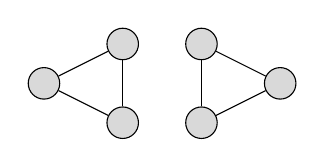
\begin{tikzpicture}[x=1cm,y=1cm] 
				\begin{scope}[scale=1.0]
				
				\tikzstyle{mycircle}=[circle,
				draw=black,
				fill=gray,
				fill opacity = 0.3,
				text opacity=1,
				inner sep=0pt,
				minimum size=4mm,
				font=\small
				]
				\tikzstyle{mycirclewhite}=[circle,
				draw=black,
				text opacity=1,
				inner sep=0pt,
				minimum size=4mm,
				font=\small
				]
				
				\coordinate (pa1) at (0, 0.5);
				\coordinate (pa2) at (1, 0);
				\coordinate (pa3) at (1, 1);
				
				\coordinate (pb1) at (2, 0);
				\coordinate (pb2) at (3, 0.5);
				\coordinate (pb3) at (2, 1);		
				
				\node[mycircle] (a1) at (pa1) {};
				\node[mycircle] (a2) at (pa2) {};
				\node[mycircle] (a3) at (pa3) {};
				
				\node[mycircle] (b1) at (pb1) {};
				\node[mycircle] (b2) at (pb2) {};
				\node[mycircle] (b3) at (pb3) {};		
				
				\draw[-] (a1) -- (a2);
				\draw[-] (a2) -- (a3);
				\draw[-] (a3) -- (a1);
				
				\draw[-] (b1) -- (b2);
				\draw[-] (b2) -- (b3);
				\draw[-] (b3) -- (b1);
				
				\end{scope}
				\end{tikzpicture}
				\caption{$G_1$ - Two disconnected circles, each of length three.}	
				\label{fig:counterExampleWLCai0}
			\end{figure}
		\end{minipage}
		\begin{minipage}{.45\textwidth} % Cai Example 2
			\begin{figure}[H]
				\centering
				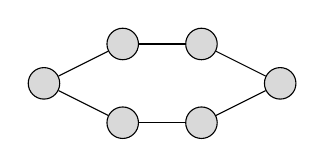
\begin{tikzpicture}[x=1cm,y=1cm] 
				\begin{scope}[scale=1.0]
				
				\tikzstyle{mycircle}=[circle,
				draw=black,
				fill=gray,
				fill opacity = 0.3,
				text opacity=1,
				inner sep=0pt,
				minimum size=4mm,
				font=\small
				]
				\tikzstyle{mycirclewhite}=[circle,
				draw=black,
				text opacity=1,
				inner sep=0pt,
				minimum size=4mm,
				font=\small
				]
				
				\coordinate (pa1) at (0, 0.5);
				\coordinate (pa2) at (1, 0);
				\coordinate (pa3) at (2, 0);		
				\coordinate (pa4) at (3, 0.5);
				\coordinate (pa5) at (2, 1);
				\coordinate (pa6) at (1, 1);		
				
				\node[mycircle] (a1) at (pa1) {};
				\node[mycircle] (a2) at (pa2) {};
				\node[mycircle] (a3) at (pa3) {};		
				\node[mycircle] (a4) at (pa4) {};
				\node[mycircle] (a5) at (pa5) {};
				\node[mycircle] (a6) at (pa6) {};		
				
				\draw[-] (a1) -- (a2);
				\draw[-] (a2) -- (a3);
				\draw[-] (a3) -- (a4);
				\draw[-] (a4) -- (a5);
				\draw[-] (a5) -- (a6);
				\draw[-] (a6) -- (a1);
				
				\end{scope}
				\end{tikzpicture}
				\caption{$G_2$ - A circle of length six.}	
				\label{fig:counterExampleWLCai1}
			\end{figure}		
		\end{minipage}

	\subsubsection{Weisfeiler-Leman Labeling Tree} \label{subsubsec:def_WLLT}
				
		The method is based on the hierarchy of the WL-labels which are constructed by the $1$-dimensional WL-labeling scheme (see algorithm \ref{alg:WLlabeling}).
		This hierarchy can be represented by a hierarchy tree, which we call \textbf{Weisfeiler-Leman labeling tree} (\textbf{WLLT}).
		The WLLT is used in the l-WWLLT method to organize and distinguishing between representations for graphs in a given dataset.
		
		In order to construct a WLLT, we require $D>0$ iterations of WL-labelings on a non-empty database of graphs $\mathcal{G}$.
		Labeled and un-labeled graphs can be treated in the same way, by considering vertex labels as the zeroth WL-labels.
		A WLLT is a rooted tree $T$, where the root is an artificial label. 
		The $i$-th layer of $T$ consists of all WL-labels arising in iteration $i$ of the labeling in any graph in $\mathcal{G}$.
		That is, there exists an edge $(l,l^\prime)$ in $T$ between vertices $l$ and $l^\prime$ if there exists a vertex $v\in V(G)$ in some graph $G\in\mathcal{G}$ and $i\in\IN$ with $l=\ell_i(v)$ and $l^\prime=\ell_{i+1}(v)$.
		The complete construction of the WLLT is sketched in algorithm \ref{alg:WLLTconstruction}.
		
		\begin{algorithm}[H]
			\caption{WLLT construction} \label{alg:WLLTconstruction} 
			\begin{tabbing}
				\textbf{Output:} \= \kill 
				\textbf{Input:} \>a graph dataset $\mathcal{G}$,\\
				\>WL-labelings $\ell_0, \dots \ell_D$ up to depth $D$.\\
				\textbf{Output:} \>WLLT $T$ of height $k$ (unweighted).
			\end{tabbing}	
			\begin{algorithmic}[1]		
				\State Initialize the WLLT as a single root $T=({r}, \emptyset)$
				\For {$G$ in $\mathcal{G}$}
					\For {$i=0$ to $D$}
						\For {$l\in \{ \ell_i(v) | \ v\in V(G) \}$}
							\If {$l\notin T$}
								\State $V(T) = V(T) \cup \{ l \}$
								\State $E(T) = E(T) \cup (p, l)$ where $\ell_{i-1}(v)=p$ and $\ell_{i}(v)=l$ 
							\EndIf					
						\EndFor
					\EndFor
				\EndFor
				\State \textbf{return} $T$
			\end{algorithmic}
		\end{algorithm}
		
		The $i$-th WL-label of vertex $v$ is given by $\ell_i(u)$.		
		Recall, that we use $\Sigma_i$ to denote the set of WL-labels of iteration $i$.
		This set relates to the $i$-th layer $T$.		
		
		Notice that if two vertices have different WL-labels in one refinement step, this implies that they have different WL-labels in all later refinement steps~\cite{1968_Weisfeiler_CONF, 2016_Kriege_NIPS}.
		For a proof by contradiction assume that two WL-labels for two vertices $v$ and $w$ in iteration $j$ are equal ($\ell_j(v) = \ell_j(w)$), but different in any previous iteration $i<j$ ($\ell_i(v) \neq \ell_i(w)$).
		Without loss of generality, say $i$ is maximal and $j$ minimal in this property and thus $i = j-1$.
		But now it is:
		\begin{flalign*}
			\ell_j(v)  &=	 \operatorname{hash}\big(\ell_{j-1}(v),\:\mset{\ell_{j-1}(n)| \ n\in\mathcal{N}_G(v)\:} \big)\\
					   &\neq \operatorname{hash}\big(\ell_{j-1}(w),  \mset{\ell_{j-1}(n)| \ n\in\mathcal{N}_G(w)} \big) &&\text{since }\ell_{j-1}(v)\neq \ell_{j-1}(w)\\
					   &= \ell_j(w)
		\end{flalign*}
		This implies that $\ell_j(v)\neq \ell_j(v)$, which contradicts the assumptions.		
		\[ \forall u,v \in V \ \forall i\in \IN: \quad \ell_k(u)\neq \ell_k(v) \implies \ell_{k+1}(u)\neq \ell_{k+1}(v) \]
		
		\begin{figure}[H]	% Three Graphs and their WL-labels
			\centering
			\begin{tikzpicture}[xscale=0.8, yscale=0.9]
			\centering
			\foreach \shiftamount/\step in {(0,0)/1, (4,0)/2, (8,0)/3}{
				\begin{scope}[shift={\shiftamount}, scale=.80]
				
				\tikzstyle{mycircle}=[circle,
				draw=black,
				fill=white,
				fill opacity=0.4,
				text opacity=1,
				inner sep=0pt,
				minimum size=4mm,
				font=\small
				]	
				
				\coordinate (ptitle) at (1, 0);
				\coordinate (pG1) at (-1.5, 7.5);
				\coordinate (pG2) at (-1.5, 4.5);
				\coordinate (pG3) at (-1.5, 1.5);
				
				\node[rectangle] (title) at (ptitle) {k=\step};
				
				\ifthenelse{\step=1}{
					\node[rectangle] (G1) at (pG1) {$G_1$};
					\node[rectangle] (G2) at (pG2) {$G_2$};
					\node[rectangle] (G3) at (pG3) {$G_3$};
				}
				
				\coordinate (pa1) at (0, 7);
				\coordinate (pa2) at (1, 8);
				\coordinate (pa3) at (2, 7);
				
				\coordinate (pb1) at (0, 4);
				\coordinate (pb2) at (0.5, 5);
				\coordinate (pb3) at (1.5, 5);
				\coordinate (pb4) at (2, 4);
				
				\coordinate (pc1) at (0, 1);
				\coordinate (pc2) at (1, 2);
				\coordinate (pc3) at (2, 2);
				\coordinate (pc4) at (2, 1);		
				
				\node[mycircle] (a1) at (pa1) {};
				\node[mycircle] (a2) at (pa2) {};
				\node[mycircle] (a3) at (pa3) {};
				
				\node[mycircle] (b1) at (pb1) {};
				\node[mycircle] (b2) at (pb2) {};
				\node[mycircle] (b3) at (pb3) {};		
				\node[mycircle] (b4) at (pb4) {};	
				
				\node[mycircle] (c1) at (pc1) {};
				\node[mycircle] (c2) at (pc2) {};
				\node[mycircle] (c3) at (pc3) {};		
				\node[mycircle] (c4) at (pc4) {};	
				
				\path[draw] (a1) -- (a2) -- (a3);
				\path[draw] (b1) -- (b2) -- (b3) -- (b4);
				\path[draw] (c3) -- (c2) -- (c4) -- (c1) -- (c2);
				
				\ifthenelse{\step=2}{		
					\node[mycircle, fill=green]  (a1) at (pa1) {$1$};
					\node[mycircle, fill=blue]   (a2) at (pa2) {$2$};
					\node[mycircle, fill=green]  (a3) at (pa3) {$1$};
					
					\node[mycircle, fill=green]  (b1) at (pb1) {$1$};
					\node[mycircle, fill=blue]   (b2) at (pb2) {$2$};
					\node[mycircle, fill=blue]   (b3) at (pb3) {$2$};		
					\node[mycircle, fill=green]  (b4) at (pb4) {$1$};	
					
					\node[mycircle, fill=blue]   (c1) at (pc1) {$2$};
					\node[mycircle, fill=yellow] (c2) at (pc2) {$3$};
					\node[mycircle, fill=green]  (c3) at (pc3) {$1$};		
					\node[mycircle, fill=blue]   (c4) at (pc4) {$2$};
				}{}
				\ifthenelse{\step=3}{		
					\node[mycircle, fill=red]    (a1) at (pa1) {$4$};
					\node[mycircle, fill=pink] (a2) at (pa2) {$6$};
					\node[mycircle, fill=red]    (a3) at (pa3) {$4$};
					
					\node[mycircle, fill=red]    (b1) at (pb1) {$4$};
					\node[mycircle, fill=violet] (b2) at (pb2) {$7$};
					\node[mycircle, fill=violet] (b3) at (pb3) {$7$};		
					\node[mycircle, fill=red]    (b4) at (pb4) {$4$};	
					
					\node[mycircle, fill=brown] (c1) at (pc1) {$8$};
					\node[mycircle, fill=lime]  (c2) at (pc2) {$9$};
					\node[mycircle, fill=gray]  (c3) at (pc3) {$5$};		
					\node[mycircle, fill=brown] (c4) at (pc4) {$8$};
				}{}	
				%		red, green, blue, cyan, magenta, yellow, black, gray, darkgray, lightgray, brown, lime, olive, orange, pink, purple, teal, violet and white
				\end{scope}	
			}		
			\end{tikzpicture}
			\caption{Examplary WL-labeling on three graphs.}	
			\label{fig:WLlabelingscheme}
		\end{figure}
				
		\begin{figure}[H]
			\centering
			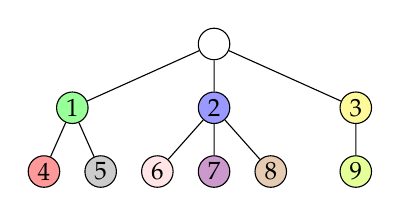
\begin{tikzpicture}[xscale=0.8, yscale=0.9]	
				\begin{scope}[scale=.90]
				
				\tikzstyle{mycircle}=[circle,
				draw=black,
				fill=white,
				fill opacity=0.4,
				text opacity=1,
				inner sep=0pt,
				minimum size=4mm,
				font=\small
				]	
				
				\coordinate (pt01) at (3, 2);
				
				\coordinate (pt11) at (0.5, 1);
				\coordinate (pt12) at (3, 1);
				\coordinate (pt13) at (5.5, 1);
				
				\coordinate (pt21) at (0, 0);
				\coordinate (pt22) at (1, 0);
				\coordinate (pt23) at (2, 0);
				\coordinate (pt24) at (3, 0);
				\coordinate (pt25) at (4, 0);
				\coordinate (pt26) at (5.5, 0);	
				
				\node[mycircle] (t01) at (pt01) {};
				
				\node[mycircle, fill=green]  (t11) at (pt11) {$1$};
				\node[mycircle, fill=blue]   (t12) at (pt12) {$2$};
				\node[mycircle, fill=yellow] (t13) at (pt13) {$3$};
				
				\node[mycircle, fill=red]    (t21) at (pt21) {$4$};
				\node[mycircle, fill=gray]   (t22) at (pt22) {$5$};
				\node[mycircle, fill=pink]   (t23) at (pt23) {$6$};
				\node[mycircle, fill=violet] (t24) at (pt24) {$7$};
				\node[mycircle, fill=brown]  (t25) at (pt25) {$8$};
				\node[mycircle, fill=lime]   (t26) at (pt26) {$9$};
				
				\path[draw] (t11) -- (t01) -- (t12);
				\path[draw] (t13) -- (t01);
				
				\path[draw] (t21) -- (t11) -- (t22);
				\path[draw] (t23) -- (t12) -- (t24);
				\path[draw] (t25) -- (t12);
				\path[draw] (t26) -- (t13);
				
				%		red, green, blue, cyan, magenta, yellow, black, gray, darkgray, lightgray, brown, lime, olive, orange, pink, purple, teal, violet and white
				\end{scope}
			\end{tikzpicture}
			\caption{WLLT to the graphs in figure \ref{fig:WLlabelingscheme}.}
			\label{fig:WLLT}
		\end{figure}
		\begin{figure}[H]
			\centering
			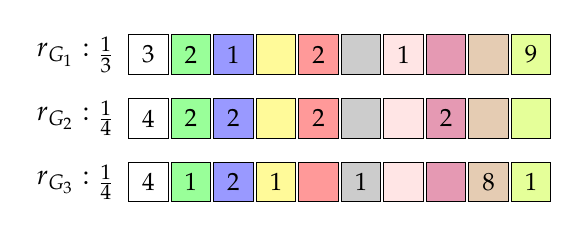
\begin{tikzpicture}[xscale=0.6, yscale=0.9]	
				\begin{scope}[scale=.90]
				
				\tikzstyle{mybox}=[rectangle,
				draw=black,
				fill=white,
				fill opacity=0.4,
				text opacity=1,
				inner sep=0pt,
				minimum size=5mm,
				font=\small
				]	
				
				\coordinate (pg1) at (0, 2); \coordinate (pf1) at (1, 2);
				\coordinate (pg2) at (0, 1); \coordinate (pf2) at (1, 1);
				\coordinate (pg3) at (0, 0); \coordinate (pf3) at (1, 0);
				
				\coordinate (pg1l0) at (2,  2);
				\coordinate (pg1l1) at (3,  2);
				\coordinate (pg1l2) at (4,  2);
				\coordinate (pg1l3) at (5,  2);
				\coordinate (pg1l4) at (6,  2);
				\coordinate (pg1l5) at (7,  2);
				\coordinate (pg1l6) at (8,  2);
				\coordinate (pg1l7) at (9,  2);
				\coordinate (pg1l8) at (10, 2);
				\coordinate (pg1l9) at (11, 2);
				
				\coordinate (pg2l0) at (2,  1);
				\coordinate (pg2l1) at (3,  1);
				\coordinate (pg2l2) at (4,  1);
				\coordinate (pg2l3) at (5,  1);
				\coordinate (pg2l4) at (6,  1);
				\coordinate (pg2l5) at (7,  1);
				\coordinate (pg2l6) at (8,  1);
				\coordinate (pg2l7) at (9,  1);
				\coordinate (pg2l8) at (10, 1);
				\coordinate (pg2l9) at (11, 1);
				
				\coordinate (pg3l0) at (2,  0);
				\coordinate (pg3l1) at (3,  0);
				\coordinate (pg3l2) at (4,  0);
				\coordinate (pg3l3) at (5,  0);
				\coordinate (pg3l4) at (6,  0);
				\coordinate (pg3l5) at (7,  0);
				\coordinate (pg3l6) at (8,  0);
				\coordinate (pg3l7) at (9,  0);
				\coordinate (pg3l8) at (10, 0);
				\coordinate (pg3l9) at (11, 0);
				
				\node (g1) at (pg1) {$r_{G_1}:$}; \node (gf1) at (pf1) {$\frac{1}{3}$};
				
				\node[mybox, fill=white]  (g1l0) at (pg1l0) {$3$};
				
				\node[mybox, fill=green]  (g1l1) at (pg1l1) {$2$};
				\node[mybox, fill=blue]   (g1l2) at (pg1l2) {$1$};
				\node[mybox, fill=yellow] (g1l3) at (pg1l3) {};
				
				\node[mybox, fill=red] 		(g1l4) at (pg1l4) {$2$};
				\node[mybox, fill=gray] 	(g1l5) at (pg1l5) {};
				\node[mybox, fill=pink] 	(g1l6) at (pg1l6) {$1$};
				\node[mybox, fill=purple] 	(g1l7) at (pg1l7) {};
				\node[mybox, fill=brown] 	(g1l8) at (pg1l8) {};
				\node[mybox, fill=lime] 	(g1l9) at (pg1l9) {$9$};
				
				\node (g2) at (pg2) {$r_{G_2}:$}; \node (gf2) at (pf2) {$\frac{1}{4}$};
				
				\node[mybox, fill=white]  (g2l0) at (pg2l0) {$4$};
				
				\node[mybox, fill=green]  (g2l1) at (pg2l1) {$2$};
				\node[mybox, fill=blue]   (g2l2) at (pg2l2) {$2$};
				\node[mybox, fill=yellow] (g2l3) at (pg2l3) {};
				
				\node[mybox, fill=red]    (g2l4) at (pg2l4) {$2$};
				\node[mybox, fill=gray]   (g2l5) at (pg2l5) {};
				\node[mybox, fill=pink]   (g2l6) at (pg2l6) {};
				\node[mybox, fill=purple] (g2l7) at (pg2l7) {$2$};
				\node[mybox, fill=brown]  (g2l8) at (pg2l8) {};
				\node[mybox, fill=lime]   (g2l9) at (pg2l9) {};
				
				
				\node (g3) at (pg3) {$r_{G_3}:$}; \node (gf3) at (pf3) {$\frac{1}{4}$};
				
				\node[mybox, fill=white]  (g3l0) at (pg3l0) {$4$};
				
				\node[mybox, fill=green]  (g3l1) at (pg3l1) {$1$};
				\node[mybox, fill=blue]   (g3l2) at (pg3l2) {$2$};
				\node[mybox, fill=yellow] (g3l3) at (pg3l3) {$1$};
				
				\node[mybox, fill=red]    (g3l4) at (pg3l4) {};
				\node[mybox, fill=gray]   (g3l5) at (pg3l5) {$1$};
				\node[mybox, fill=pink]   (g3l6) at (pg3l6) {};
				\node[mybox, fill=purple] (g3l7) at (pg3l7) {};
				\node[mybox, fill=brown]  (g3l8) at (pg3l8) {$8$};
				\node[mybox, fill=lime]   (g3l9) at (pg3l9) {$1$};
				
				%		red, green, blue, cyan, magenta, yellow, black, gray, darkgray, lightgray, brown, lime, olive, orange, pink, purple, teal, violet and white
				\end{scope}
			\end{tikzpicture}
			\caption{Graph representations of the graphs in figure \ref{fig:WLlabelingscheme}\\with respect to the WLLT in figure \ref{fig:WLLT}.}
			\label{fig:GraphRepresentations}
		\end{figure}
		
		In this thesis, we restrict ourselves to the case that the given graph dataset contains labeled graphs.
		The set of these initial labels can be interpreted as zeroth WL-labels and the set of the vertices of the first layer in a corresponding WLLT ($\Sigma_0$).
		Notice that these have depth $1$ in the WLLT and further layers of depth $D$ correspond to the D-1-th WL-labeling.
		
		Figures \ref{fig:plotwlltl2e0aids2915h-25m} and \ref{fig:plotwlltmutagl2} display two examples of WLLTs.
		Both examples display the tree for depth $D=2$, and thus with two layers.
		Notice, how the much bigger and diverse dataset AIDS generates a much bigger tree than the dataset MUTAG with the same number of WL-labeling iterations.
		
		As mentioned before, the l-WWLLT method aims to define meaningful distances between the WL-labels in the WLLT by adjusting weights on its edges.		
		An example of a weighted WLLT is shown in figure \ref{fig:plotwlltmutagl2weighted}.
		The edge colors and edge lengths correspond to the edge weights.
		
		\begin{figure}[H]
			\centering
			\begin{subfigure}{0.49\textwidth}
				\centering
				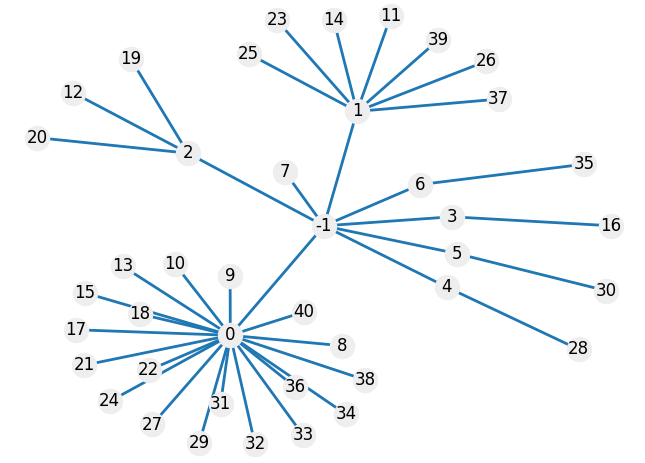
\includegraphics[width=1.0\linewidth]{images/plot_wllt_MUTAGl2}
				\caption{Example WLLT: MUTAG, $d=2$.}
				\label{fig:plotwlltmutagl2}
			\end{subfigure}
			\begin{subfigure}{0.49\textwidth}
				\centering
				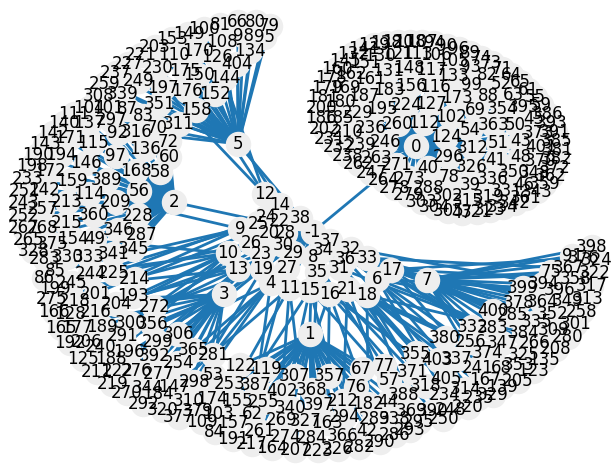
\includegraphics[width=1.0\linewidth]{images/plot_wllt_l2_e0_AIDS_29_15h-25m}
				\caption{Example WLLT: AIDS, $d=2$.}
				\label{fig:plotwlltl2e0aids2915h-25m}
			\end{subfigure}
			\caption{Unweighted WLLT examples}\label{fig:combined}
		\end{figure}
		
		\begin{figure}[H]
			\centering
			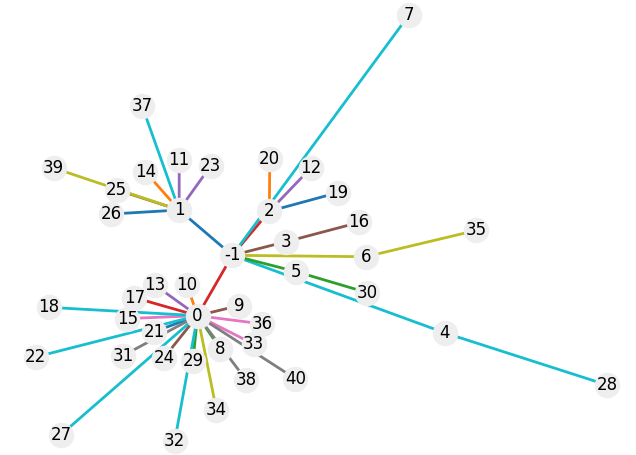
\includegraphics[width=0.7\linewidth]{images/plot_wllt_MUTAGl2_weighted}
			\caption{Weighted WLLT example: AIDS, $d=2$.}
			\label{fig:plotwlltmutagl2weighted}
		\end{figure}
		
		\paragraph{Runtime of the WLLT Construction}	
		As shown in section \ref{subsubsec:def_WLlabeling}, the computation of $d$ iterations of WL-labels for a graph with $m$ edges can be done in $\mathcal{O}(dm)$.
		Using non-negative integers as WL-labels allows for an easy construction of the WL-label hierarchy (parent list) in linear time.
		The definition of edge weights requires to initialize $p$ values, if the WLLT holds $p$ many WL-labels and the (possibly artificial) root.
		Depending on the desired initialization, the edge weights can be defined during the construction.
		For a more sophisticated initialization note, we may limit $p$ by the number of WL iterations, and the total number of vertices in the whole graph dataset.
		A stricter limitation of $p$ is not useful, if the initialization method is not specified.		
		Thus we conclude that for a graph dataset $\mathcal{G}$ of $N$ graphs with at most $m$ edges, the WLLT can be constructed with uniform weights in $\mathcal{O}(Ndm)$.
		
\subsection{Kernels} \label{subsec:def_kernels}

	A function $f:\IR\to\IC$ is called \textbf{positive-definite} if for any real numbers $x_1,\dots, x_n$ the matrix 
	$A = [a_{i,j}]^n_{i,j=1}$ with $a_{i,j} = f(x_i-x_j)$ is positive \textbf{semi-definite}, that is $x^\intercal A x \ge 0$ for all $x\in\IR^n$.
	In case of a symmetric matrix, this implies that it is positive definite if all its eigenvalues are non-negative.
	If it further is $x^\intercal A x = 0$ only for $0=x\in\IR^n$, the matrix is called \textbf{strictly positive definite}~\cite{2008_Hofmann_CONF}. %Other definitions: 2019_Togninalli_NIPS - Appendix A1
	A function $f$ is (\textbf{strictly}) \textbf{negative-definite} if $-f$ is (strictly) positive-definite~\cite{2007_Borgwardt_BOOK}.	
		
	Kernels are similarity functions that can be interpreted as a dot product in a high-dimensional space.
	They are often used in learning algorithms that rely on dot products, such as classifications tasks using support vector machines (SVMs)~\cite{2002_Scholkopf_CONF, 2019_Togninalli_NIPS}.
	Other applications are regression~\cite{1996_Drucker_CONF}, clustering~\cite{1996_Vapnik_CONF} and principal component analysis~\cite{1997_Schoelkopf_CONF}.
	
	Formally, a \textbf{kernel} on a set $X$ is a function $k:X\times X \to\IR$ such that there is a (reproducing) real Hilbert space $\mathcal{H}$ and a mapping $\phi:X\to\mathcal{H}$ (feature map) such that $k(x,y) = \langle \phi(x), \phi(y) \rangle_\mathcal{H}$ for all $x, y\in X$~\cite{1999_Haussler_CONF, 2008_Hofmann_CONF}. 
	Here, $\langle \cdot,\cdot \rangle_\mathcal{H}$ denotes the inner product of $\mathcal{H}$.
	The definition of definiteness extends from matrices to kernels, in terms of the Gram matrix or kernel matrix $K:=\big[ k(x, y) \big]_{x, y}$~\cite{2008_Hofmann_CONF}.
	Equivalently, a function $k:X\times X\to\IR$ is a kernel if and only if for every subset $\{x_1, \dots, x_n\}\subseteq X$ the matrix $\big[k(x_i, x_j)\big]^n_{i,j=1}$ is positive semi-definite~\cite{2016_Kriege_NIPS, 2019_Togninalli_NIPS}.
	$\big[k(x_i, x_j)\big]^n_{i,j=1}$ is called \textbf{Gram matrix} of $k$ with respect to $x_1, \dots, x_n$.
	Or in other words a symmetric function $k:X\times X\to\IR$ is called a positive definite kernel, if
	\begin{equation} \label{eq:pd_kernel}
		\forall c_i\in\IR \; \forall n\in\IN \; \forall x_i\in X:\qquad \sum_{i,j=1}^{n} c_i c_j k(x_i, x_j) \ge 0
	\end{equation}
	With respect to kernel a kernel function $k$ we call it \textbf{conditional positive definite}, if it satisfies equation \ref{eq:pd_kernel} for all $c_i\in\IR$ with $\sum_{i=1}^{n} c_i = 0$~\cite{2019_Togninalli_NIPS}.
	The \textbf{Dirac Kernel} $k_{\delta}$ is defined by $k_{\delta}(x,y)=1$, if $x=y$ and $0$ otherwise.
	
	A \textbf{graph kernel} on a set of graphs $\mathcal{G}$ is a symmetric, positive semidefinite kernel $k:\mathcal{G}\times \mathcal{G}\to \IR$ with domain $\mathcal{G}$.
	Notice that graph kernels can be defined on both the vertices or the edges of a graph~\cite{2008_Hofmann_CONF} and in general do not need to be positive (semi-)definite.	
	But if they are, one can use the so-called kernel trick, by representing the computation as an inner product in a any Hilbert space.
	This is most useful for high dimensional feature spaces, since the explicit computation for associated feature maps usually involves high costs~\cite{2003_Gaertner_CONF}.
	However for example the Optimal Assignment Kernel proved useful, despite being not positive definite in general (see ~\cite{2005_Froehlich_ICML})~\cite{2018_Vert_CONF}.
	
	\subsubsection{Laplacian Kernel} \label{subsec:def_LaplacianKernel}
		
		The \textbf{Laplacian Kernel} has favorable conditions for positive definiteness in the case of non-Euclidean distances~\cite{1984_Berg_BOOK, 2015_Feragen_IEEE}, and when using noiseless data~\cite{2015_Rupp_CONF}.
		Since many graph similarity measure, as well as the l-WWLLT distance, may not be an Euclidean distance, this kernel is useful to derive a kernel from such a proposed graph similarity measure.
		It is defined as:		
		\begin{equation}\label{eq:LaplacianKernel}
		k(x,y) = \exp\big( -\lambda d(x,y) \big)
		\end{equation}
		\citeauthor{1938_Schoenberg_CONF} showed that the Laplacian Kernel is positive definite for all $0<\lambda\in\IR$, if and only if the ground distance $d$ is (conditional) negative definite.
		For a proof of this claim see \cite{1938_Schoenberg_CONF} and Theorem C.3.2 in \cite{2017_Bollobas_BOOK}.
	
	\subsubsection{Tree-sliced Wasserstein Kernel} \label{sec:def_TSWKernel}
	
		Recall equation \ref{eq:TreeWassDist} for the definition of the negative definite Tree Wasserstein Distance.
		\citeauthor{2019_Le_NIPS} proposed a the \textbf{Tree-sliced Wasserstein Distance} % Definition 1. page 4
		\begin{equation} \label{eq:TreeSlicedWassersteinDistance}
			\text{TSW}(\mu, \nu) := \frac{1}{n}\sum_{i=1}^{n}\mathbb{W}_{d_{T_i}}(\mu, \nu)
		\end{equation}
		Using it in the Laplacian kernel (equation \ref{eq:LaplacianKernel}) results in the \textbf{Tree-sliced-Wasserstein} (\textbf{TSW}) \textbf{Kernel} $k_{\text{TSW}}$~\cite{2019_Le_NIPS}:
		\[ k_{\text{TSW}}(\mu, \nu) := \exp\big( -\lambda \text{TSW}(\mu, \nu) \big) \]
		
		Since we define the l-WWLLT as an instance of the Tree-sliced Wasserstein Kernel, it is important to notice that this kernel is positive definite.		
		As mentioned in section \ref{subsec:def_LaplacianKernel}, the Laplacian kernel is positive definite for all $\lambda>0$, if and only if the ground distance $d$ is (conditional) negative definite.		
		This in turn highly depends on the used ground metric.
		For example, Wasserstein distances with discrete metrics as ground distances are conditional negative definite~\cite{2018_Gardner_IEEE}. 		
		\citeauthor{2019_Le_NIPS} showed that the Tree Wasserstein distance is negative definite (Proposition 2 in ~\cite{2019_Le_NIPS} following~\cite{1984_Berg_BOOK} on pages 66-67), 		
		and thus also conditionally negative definite.
		Since the Tree-sliced Wasserstein Distance is thus a sum of negative definite functions, it is negative definite itself and the TSW Kernel is positive definite as desired.
		
	% WL Graph Kernels - 2011_Shervashidze_JMLR
	\subsubsection{Weisfeiler-Leman Graph Kernel} \label{subsec:def_WLkernel}
		For $d$ iterations of the WL-labeling scheme, lets call a graph $G$ with the WL-labeling of the $i$-th iteration the \textbf{WL graph at depth} $i$:
		\[ G_i = (V,E,l_i) \]
		Furthermore lets define the \textbf{WL-sequence up to height $i$} of set graph $G$ as the sequence:
		\[ ( G_0,G_1,\dots,G_i ) \ = \ ( (V,E,\ell_0),(V,E,\ell_1), \dots,(V,E,\ell_i) ) \]
		As said before, we consider the original labels of a graph $G=(V,E,L)$ as labels of the zeroth WL iteration ($L=\ell_0$).
		
		Let $k$ be any positive semi-definite kernel on two graphs $G$ and $H$. 
		Then the \textbf{Weisfeiler-Leman} (\textbf{WL}) \textbf{Graph Kernel}~\cite{2011_Shervashidze_JMLR} with $D$ iterations with $k$ as base kernel is defined as
		\[ k_{\text{WL}}^{(D)}(G, H) \ = \sum_{i=0}^{D} k(G_i,H_i) \]
		A more general definition can be derived, when weighting the WL iterations with $0\le \alpha_i\in \IR$:
		\[ k_{\text{WL}}^{(D)}(G, H) \ = \sum_{i=0}^{D} \alpha_i k(G_i,H_i) \]
		This weight function allows for example to emphasize larger substructures, which are represented by WL-labels from deeper WL iterations~\cite{2021_Schulz_CONF}.
	
%		\paragraph{Weisfeiler-Leman Subtree Graph Kernel} %LaterTODO GENERAL kernel From where comes the first definition?
%		Again let $G$ and $H$ be two graphs.
%		Recall, that in this thesis we define the WL-labels, such that all $\Sigma_i$ are pairwise disjoint.
%		We require this property in the following definition.
%		Define for every $i$, $\Sigma_i=(\sigma_{i,1},\dots,\sigma_{i|\Sigma_i|})$ as the ordered tuple of the set $\Sigma_i$.
%		Define a map $c_i: \{G, H\}\times \Sigma_i\to\IN$ such that $c_i(G,\sigma_{i,j})$ is the number of occurrences of the WL label $\sigma_{i,j}$ in the graph $G$.
%		The \textbf{Weisfeiler-Leman Subtree} (\textbf{WLST}) \textbf{Graph Kernel} on $G$ and $H$ for $D$ WL-labeling iterations is defined as:
%		\[ k_{\text{WLST}}^{(d)}(G,H) \ = \ \langle \psi_{\text{WLST}}^{(d)}(G), \psi_{\text{WLST}}^{(d)}(H) \rangle \]
%		where \[ \psi_{\text{WLST}}^{(d)}(G) = \big( c_0(G,\sigma_{0,1}),\dots, c_0(G,\sigma_{0,|\Sigma_0| }),\dots,c_h(G,\sigma_{h,1}),\dots, c_h(G,\sigma_{h,|\Sigma_h| }) \big) \]
%		In other words, the WLST Kernel counts the common (original and) WL-labels in the two graphs.
%		%Note that due to the runtime of algorithm \ref{alg:WeisfeilerLemanEmbedding}, one can compute the WL-Subtree Kernel in $\mathcal{O}(dm)$.
%		
%		One can show that the WL Kernel and the WLST Kernel are closely related.
%		Let $k$ be a function to count pairs of matching vertex labels in two graphs:
%		\[ k(G,H) := \sum_{v\in V(G)}\sum_{w\in V(H)} \delta\big( \ell(v), \ell(w) \big) \]
%		Then $k_{\text{WL}}^{(d)}(G,H) = k_{\text{WLST}}^{(d)}(G,H)$. %LaterTODO: Prove?
%		
%		Let $\mathcal{G}$ be a set of graphs and $\Theta_i$ a set of hard clustering functions (i.e. partitionings) of the set of depth-$i$ unfolding trees $\mathcal{T}^{(i)}$ appearing in the graphs in $\mathcal{G}$.
%		Regard each element of $\Theta_i$ as a function $\rho:\mathcal{T}:\Sigma_i\to [k]$, where $k$ is the number of clusters defined by $\rho$.
%		Then, for any graphs $G, H\in\mathcal{G}$ and depth parameter $d\in\IN$, the \textbf{relaxed Weisfeiler-Leman Subtree} (R-WLST) \textbf{Kernel}~\cite{2021_Schulz_CONF} is defined as:
%		\[ k^d_{\text{R-WLST}}(G,H) = \sum\limits_{i=0,\dots, d}\sum\limits_{\rho\in\Theta_i}\sum\limits_{v\in V(G)}\sum\limits_{w\in V(H)} \delta\Big( \rho\big( T^i(G,v)\big),\; \rho\big( T^i(H,w)\big) \Big) \]
%		$k^d_{\text{R-WLST}}$ is positive semi-definite and equivalent to the original WL-Subtree Kernel for $\Theta_i=\{\rho_i\}$. %LaterTODO: prove
	
	% WL-OA - 2016_Kriege_NIPS
	\subsubsection{Weisfeiler-Leman Optimal Assignment Graph Kernel} \label{subsec:def_WLOA}
		The \textbf{Weisfeiler-Leman Optimal Assignment} (\textbf{WL-OA}) \textbf{Graph Kernel} proposed by \citeauthor{2016_Kriege_NIPS} is similarly based on the hierarchy implied by the WL-labels~\cite{2016_Kriege_NIPS}.		
		To understand the difference to the approach in this thesis, we briefly summarize the definition of the WL-OA.
		Consider two graphs $G$ and $H$ and their vertex sets $V(G)$, $V(H) \subseteq\mathcal{V}$.
		Let $\mathcal{B}\big(V(G), V(H)\big)$ denote the set of all bijections between $V(G)$, $V(H)$.
		Given $d$ iterations of the WL-labeling scheme for two vertices $v,w\in\mathcal{V}$, define the base kernel of the WL-OA as the sum of equal WL-labels over all these iterations:
		\[ k_d(v,w) := \sum_{i=0}^{d} k_{\delta}\big( \ell^i(v), \ell^i(w) \big) \]
		Now the WL-OA Kernel is defined as
		\[ K(G, H) := K_{\mathcal{B}}^{k}\big( V(G), V(H) \big) = \max\limits_{B\in\mathcal{B}\big(V(G), V(H)\big)} \sum_{(v,w)\in B}k_d(v,w)  \]
		If the vertex sets have different carnality one may introduce artificial vertices $z$ to the smaller set with $k_d(z,x)=0$ for all $x\in\mathcal{V}$.
		
		Notice that $k_d(v,w)$ corresponds to the number of matching WL-labels in the refinement sequence.
		As mentioned before, if two vertices have different WL-labels at any depth, all their WL-labels in deeper depths are different too.
		Thus the WL-OA Kernel bases its similarity measure on the length of the path in the WLLT to the lowest common ancestor of the WL-labelings of two vertices.
						
	% WWL graph kernel - 2019_Togninalli_NIPS
	\subsubsection{Wasserstein Weisfeiler-Leman Graph Kernel} \label{subsec:def_WWLKernel}
		
		Similarly to the WL Graph Kernel (section  \ref{subsec:def_WLkernel}) and the WL-OA Kernel (section \ref{subsec:def_WLOA}), the \textbf{Wasserstein Weisfeiler-Leman} (\textbf{WWL}) \textbf{Graph Kernel} is constructed using WL-labels of a graphs vertices.
		Different is however, that all WL-labels are used.
		Let there be $D$ iterations of the WL-labeling scheme and consider a graph $G=(\{ v_1, \dots, v_n \}, E)$ with $n$ vertices.
		Again let $\Sigma=\IN$ be the set of all possible WL-labels.
		For a vertex $v$ in a graph $G$, define the vertex embedding $f_{\text{WL}}^{D}:V\to\Sigma^{D+1}$ as the (row) vector of all WL-labels, that are assigned to $v$:		
		\[ f_{\text{WL}}^{D}(v) = \big( \ell_0(v), \dots, \ell_D(v) \big)  \]
		Now define a graph representation $f_{\text{WL}}^{D}$ (graph embedding scheme~\cite{2019_Togninalli_NIPS}) as 
		\[ F_{\text{WL}}^{D}(G) = \begin{pmatrix}
		f_{\text{WL}}^{D}(v_1) \\ \dots \\ f_{\text{WL}}^{D}(v_n)
		\end{pmatrix}  = \big( \ell_i(v_j) \big)_{\begin{subarray}{l}
			j\in\{0,\dots,D\}\\
			i\in\{1,\dots,n\}
			\end{subarray}} \in \Sigma^{n\times (D+1)} \]
		Note that \citeauthor{2019_Togninalli_NIPS} described this graph representation as the concatenation of WL features, which are the \textit{column} vectors of all WL-labels for all vertices, in one fixed WL-labeling iteration.
		Next, we define the normalized Hamming distance $d_{\text{Ham}}: \Sigma^{(D+1)} \to \IR$ as the normalized count of equal entries in two vectors:
		\[ d_{\text{Ham}}(f_0, f_1) = \frac{1}{D+1} \sum\limits_{i=0}^{D} \delta(f_0, f_1) \]		
		For $\lambda\in \IR^+$ and using $d_{\text{Ham}}$ as ground metric for the $L^1$-Wasserstein distance (see equation \ref{eq:discreteWassDist}), we can define the WWL Kernel as:		
		\begin{equation} \label{eq:WWLKernel}
			K_{\text{WWL}}(G,H) = \exp(-\lambda \mathcal{W}(F_{\text{WL}}^{D}(G), F_{\text{WL}}^{D}(H)) )
		\end{equation}
		
		Notice, that we define the l-WWLLT distance, very similarly. 
		As ground distance, we use a tree metric, which depends on edge weights in the WLLT, which is changed by a learning process.
		Due to the nature of the used ground distance, we also switch the computation of the Wasserstein distance to the tree-sliced variation (section \ref{subsec:def_WassDist}).

\subsection{Cluster Learning} \label{subsec:def_cl_scores}

	There are many different metrics to evaluate a given clustering.
	Different scores measure the tightness or denseness, separation, and intra and inter dispersion of clusters.
	In general, we prefer clusterings with high separation and inter dispersion and with tight and dense clusters or low intra dispersion.
	We now state definitions of three cluster scores, which were used in the evaluation process.
	
	The \textbf{Silhouette coefficient} (SS) $S_{\text{SC}}$ is based on the comparison of the clusters tightness and separation~\cite{1987_Rousseeuw_ELSEVIER}.
	Let $a$ be the mean intra-cluster distance and $b$ be the distance to the nearest cluster for each sample.
	Then $S_{\text{SC}}$ is defined as
	\[ S_{\text{SC}} := \frac{ b - a }{ \max(a, b) } \quad \in[-1, 1]\]
	That is the mean of the distances between a sample and the nearest cluster that it is not a part of.
	Thus positive values close to $1$ indicate that the data is clustered in \textit{well separated} clusters, and the samples are less similar to the other samples in the assigned cluster, than the to the ones in the closest other cluster.
	Negative values indicate that a sample has been assigned to the wrong cluster, i.a. another cluster is denoted as more similar.
	Values near zero indicate \textit{overlapping clusters} - indicating that samples are cannot reliably be separated from other clusters~\cite{1987_Rousseeuw_ELSEVIER}.
	The used implementation was provided by \textbf{Scikit-Learn.org}.
	\footnote{ \url{https://scikit-learn.org/stable/modules/generated/sklearn.metrics.silhouette_score.html\#sklearn.metrics.silhouette_score},		\url{https://github.com/scikit-learn/scikit-learn/blob/f3f51f9b6/sklearn/metrics/cluster/_unsupervised.py\#L39} }
	
	The \textbf{Davies-Bouldin score} (SDB) $S_{\text{DB}}$ gives an average similarity of each cluster with its most similar cluster~\cite{1979_Davies_IEEE}.
	Let $M_{i,j}$ be the distance between characteristic vectors of cluster $i$ and $j$, and $S_i$ the dispersion of cluster $i$.
	The function
	\[ R_{i,j} := \frac{S_i + S_j}{M_{i,j}} \]
	is a non-negative, symmetric similarity function. 	
	Furthermore, the similarity expressed by $R_{i,j}$ decreases, if the distance $M_{i,j}$ between the clusters increases, while the dispersion of the individual clusters remains constant.
	Now the Davies-Bouldin score $S_{\text{DB}}$ is defined as the average maximum dis-similarity $R_{i,j}$ between all $n$ clusters:
	\[ S_{\text{DB}} := \frac{1}{n}\sum_{i=0}^{n-1}\; \max\limits_{i\neq j} R_{i,j} \] 
	Thus the score is based on the ratio of within-cluster distances to between-cluster distances and clusters which are \textit{farther apart} and \textit{less dispersed} yield a better score.
	Lower (positive) values indicate a better clustering.
	But the score is only zero if the dispersion of both clusters $i$ and $j$ vanish (that is each cluster consists of indistinguishable samples).	
	Note that the dataset must be partitioned into at least two clusters with different cluster centers for the score to have meaning.
	The used implementation was provided by \textbf{Scikit-Learn.org}.
	\footnote{ \url{https://scikit-learn.org/stable/modules/generated/sklearn.metrics.davies_bouldin_score.html},	\url{https://github.com/scikit-learn/scikit-learn/blob/f3f51f9b6/sklearn/metrics/cluster/_unsupervised.py\#L307} }
	
	The \textbf{Calinski-Harabasz score} (SCH) $S_{\text{CH}}$ (also known as variance ration criterion) is the ratio of the mean between-cluster (intra) dispersion and the within-cluster (inter) dispersion~\cite{1974_Calinski_CONF}.
	Let $n$ be the size of the dataset and $k\ge 1$ the number of clusters. 
	For cluster $i$ let $C_i$ be the set of data points in it, $c_i$ its the center and $n_i$ its size. Let $c_D$ be the center of the whole dataset.
	Then define the \textit{between group dispersion matrix} as
	\[ B_k := \sum_{i=0}^{k-1} n_i (c_i - c_E) (c_i - c_E)^\intercal \]
	and the \textit{within-cluster dispersion matrix} as
	\[ W_k := \sum_{i=0}^{k-1} \sum_{x \in C_i} (x - c_i) (x - c_i)^\intercal \]
	Now the Calinski-Harabasz score is defined as the 
	\[ S_{\text{CH}} = \frac{\tr\big(B_k\big)}{\tr\big(W_k\big)} \ \frac{n-k}{k-1} \]	
	The score is higher when clusters are \textit{dense} and \textit{well separated}.
	% Also, that score is generally higher for convex clusters than other concepts of clusters, such as density based clusters.	
	The used implementation was provided by \textbf{Scikit-Learn.org}.
	\footnote{ \url{https://scikit-learn.org/stable/modules/generated/sklearn.metrics.calinski_harabasz_score.html},	\url{https://github.com/scikit-learn/scikit-learn/blob/f3f51f9b6/sklearn/metrics/cluster/_unsupervised.py\#L253} }

\section{Method} \label{sec:method}

In this section, the researched method itself is explained.
Before describing important steps in the method in detail, we give an overview over the method.
The first step is to take a classified graph dataset (training set), and subjected all graphs to the WL-labeling scheme up to a specified fixed number of iterations (algorithm \ref{alg:WLlabeling}).
During this, the corresponding WLLT is constructed (algorithm \ref{alg:WLLTconstruction}).
After the complete construction of the WLLT, it is equipped with initial edge weights (section \ref{subsec:WLLT_ew_init}).
This allows to define vector representations of the graphs (section \ref{subsec:graph_representation}).
Now machine learning is applied, to iteratively update these edge weights (section \ref{subsec:EWL}).
The update decision is based on decreasing the distance between graph samples from the same class, and increasing the distance between sample from different classes.
It is crucial to notice, that changing the distance between two samples influences edge weights in the WLLT, which may be used to compute the distance between many other samples.
The performance of the learner is instead measured on the resulting distance matrix for all graphs.
Some of the used performance evaluation is presented at the end of this section, too.

\subsection{Graph Representation} \label{subsec:graph_representation}

	One of the easiest data-structures to represent complex structure data are fixed-size vectorial representations.
	Similarly to the approach used in the No-graph kernel proposed by \citeauthor{2021_Schulz_CONF}, we used a vertex label histogram as graph representations.
	However unlike the histogram used for the definition of the No-graph kernel, the vertex labels we use, compress information on the structure of the (labeled) graph.
	We define the \textbf{graph representation} (graph \textbf{feature vectors}) $r_G$ for a graph $G$ in the following way.
	Let $T$ be the WLLT with $p$ vertices ($|V(T)|=p$) and depth $D$ (i.e., $D$ iterations of WL-labelings were performed on the graph dataset).
	Note, that this includes an artificial root and $p-1$ assigned WL-labels, where the WL-labels of the zeroth iteration are the original vertex labels in the graph dataset.
	Further note, that all labels in the WLLT are distinct.	
	For a graph $G$ let $S_i$ denote the set of vertices, that were assigned the label $i$ in any of all $D$ iterations of the labeling scheme:
	\[ S_i := \{ v\in V(G)| \exists j:\ \ell_j(v)=i \} \]	
	Now define the graph representation $r_G$ of $G$ as the normalized distribution of WL-labels among the vertices of $G$:
	\begin{equation} \label{eq:graphrepr}
		r_G := \frac{1}{|V(G)|} \big( |S_0|, |S_1| \dots |S_p| \big)\ \in\IR^{p}
	\end{equation}
	For high $D$ and a diverse dataset (implying a high value of $p$), it is expected that these representations are sparse vectors.
	
\subsection{WLLT Edge Weight Initialization} \label{subsec:WLLT_ew_init}
	
	Since we measure the performance of the learner by comparison to the initial state (recall section \ref{subsec:research_question}), the initialization of the edge weights in the WLLT effect the computations and evaluations significantly.
	The edge weights are used additatively in the computation of the distance between two vertices (WL-labels) in the WLLT (recall the definition of \textbf{distance} in section \ref{subsec:def_graphtheory}). 
	Furthermore, we require non-negative edge weights for a resulting positive definite Tree-sliced Wasserstein Kernel (section \ref{subsec:def_WassDist}).
	Thus it is reasonable to initialize the edge weights with positive values.
	In all edge weights in the zeroth layer of the WLLT, that is the weights of all edges incident to the root, completely define the distances between the zeroth WL-labels.
	If initial vertex labels are known and used as zeroth WL-labels, one may use application based knowledge to initialize these edge weights.
	Otherwise, and for all other edge weights, the uniform initialization is reasonable.
	This way, the tree-structure itself ensures that WL-labels of different subtrees are further apart, which reflects the idea of the WL-labeling scheme.
	For most experiments and during the development of the method, a uniform initialization to value $1.0$ (with no prior application based knowledge) was used.
	
	Other possible initialization, like based on a gradient through the depth of the WLLT (fixed or based on the layer size) may be applicable too.
	One may assume that the learning process could be able to reach a desirable configuration, largely independently of the initialization.
	The experiments however were not extensive enough do not support this assumption empirically.

\subsection{Edge Weight Learner} \label{subsec:EWL}
	
%	For reference, the processes described in this subsection are implemented in the script \texttt{x3\_wllt\_edge\_weight\_learner.py}.	
	In order for the edge weight learning to begin, a complete WLLT (up to some depth and with edge weights), the feature vectors (section \ref{subsec:graph_representation}) of all graphs, and the graph classifications must be given.
	The outer loop in the computations performed by the edge weight learner, loops over all learning epochs and returns newly defined edge weights each time.
	Each learning epoch consists of an inner loop over the graph samples in a chosen batch of graph samples for this learning epoch.
	Since the inner loop loops over all pairs of graphs (computing their distance), the batch size enters quadratically into the calculation of the runtime of the learning process.
	Before starting the first epoch, the batches for every epoch are constructed.
	To simplify later computations, each such batch contains approximately the same number of graphs from every given class.
	If the sizes of different graph classes vary greatly, this is not ideal, with respect to an equalized weighting of the graph samples. 
	To diminish such issues, the batch sizes were chosen accordingly for the respective datasets.
	For each learning epoch, all different graph combinations of the graphs in the batch are used to compute a  weight update $\Delta w$ for the WLLT edge weights $w$:
	\[ w^\prime = w + \eta * \Delta w \]
	Here, $\eta\in(0,1]$ is the learning rate.
	Let $r_{G_0}, r_{G_1}\in\IR^p$ be the graph representations for two graphs and $w\in\IR^p$ the vector of current edge weights in the WLLT.
	Recall equation \ref{eq:TreeWassDist} with distributions $\mu = r_{G_0}$ and $\nu=r_{G_1}$.	
	Denote the weighted difference vector between the graphs as $\Delta r_{G_0, G_1} \in\IR_+$:
	\[ \IW_{d_T}( r_{G_0}, r_{G_1} ) = \sum_{e\in E} \underbrace{ w(e) \ \Big| r_{G_0} \big( \Gamma(e_c) \big) -  r_{G_1} \big( \Gamma(e_c) \big) \Big| }_{=: \Delta r_{G_0, G_1}(e)} = \sum \Delta r_{G_0, G_1} \]
	
	Now if the graphs are in the same class ($c(G_0) = c(G_1)$), their distance $\IW_{d_T}( r_{G_0}, r_{G_1} )$ shall be decreased, and increased otherwise.
	To effect as little other distances as possible, we update only the edge weights $w(e)$ where $\Delta r_{G_0, G_1}(e) \neq 0$.
	These are exactly all edge weights, which contribute in the computation of the Wasserstein distance between the considered graphs.
	Let $\delta^>$ be an indicator function such that $\delta^>(x)=\{i| x_i>0 \}$.
	If not stated otherwise, in the following we simplify the notation by writing ${w}_{\delta^>(\Delta r_{G_0, G_1})}$ as $w$.
	We use a \textbf{pull factor} $f_{\text{pull}}\in(0,1]$ and a \textbf{push factor} respectively $f_{\text{push}} \in(0,1]$ and set:
	\begin{equation} \label{eq:DeltaW}
		\Delta w = \begin{cases}
			f_{\text{pull}} w &\text{if } c(G_0) = c(G_1)\\
			f_{\text{push}} w &\text{otherwise}\\
		\end{cases}
	\end{equation}
	Notice that by definition of the push and pull factors (\textbf{pp-factors}), and the learning rate, the edge weight update is the addition or subtraction of a fraction of the already used weights.
	Thus the weights remain non-negative during all learning epochs.
	As mentioned, this is desired in order to use the resulting tree metric in the definition of a graph kernel.
	
	If the edge weights were updated after each sample, the order of sample from the same class and from different classes would matter and the batch size has effectively size one.
	To prevent this, all weight updates during one learning epoch are stored but not applied.
	Applying all updates afterwards may lead to an exponential scaling effect, which we naturally would like to avoid.
	Thus, after each epoch the mean of all computed (non-negative) updates is applied.
	
	Using the Wasserstein distance here to align the structural graph representations may be beneficial in capturing more complex characteristics of the graph, compared to taking the mean or other additive simplifications as were used for the definition of many graph convolution kernels (see related work in section \ref{subsec:related_work})~\cite{2019_Togninalli_NIPS}.
	
	\paragraph{Absolute pp-Factors}
	The described edge weight update has the benefit, that the edge weights remain non-negative all the time.
	However the definition of the weight delta as a percentage of existing weight may seem unusual.
	To compare the effects of a more traditional, additive update, such an update was implemented too.
	Using this setting in the learner, uses the following definition: 
	\begin{equation}\label{eq:DeltaW_Abs_pp_factors}
		\Delta w = \begin{cases}
			f_{\text{pull}} &\text{if } c(G_0) = c(G_1)\\
			f_{\text{push}} &\text{otherwise}\\
		\end{cases} 
	\end{equation}
	
	Since we do not need to fear exponentially de- or increasing weights in this setting, the accumulated weight updates are applied after each epoch without taking their mean.
	
	\paragraph{Class-Imbalance Factor}
	Since the update mechanism increases the edge weights for graphs from different classes and decreases the edge weights graphs from the same class, 
	depending on the number of classes and their sizes, the relation between added and removed weight may vary greatly.
	To ensure better comparability between datasets, and for example different fractions of dataset, we reduce this effect by introducing a factor which we refer to as \textbf{class imbalance factor}.
	
	Let $m$ be the batch size, and let there be $n$ (selected) graphs for every of $c$ classes in each batch.
	The number of possibilities to draw two graphs from the same class $p_S$ amounts to the number of possibilities to draw the first graph from one fixed class ($n/2$), times the number of possibilities to draw
	a second, different graph from the same class ($(n-1)/2$).
	One may summarize these possibilities to $n\choose2$ as well.
	This has to be calculated for every of the $c$ classes.
	Thus it is:
	\[ p_S = {n \choose 2} c = \frac{n(n-1)}{2} c \]
	The number of possibilities to draw two graphs from different classes $p_D$ amounts to the number of possibilities to draw two graphs, each from two different fixed classes ($nn$), times the number of possibilities to draw
	such two different classes (${c \choose 2}$).
	Thus it is:
	\[ p_D = nn{c \choose 2} = \frac{cnn(c-1)}{2} \]
	Since these factors are used only for scaling the applied weights, we ignore the common factor $nc/2$.
	Now one can scale the weight update of same class samples with $1/n-1$ and different class samples with $1/n(c-1)$.
	This however greatly decreases the weights, and in the implementation these factors were scaled, such that only different class samples are scaled by $1 / ((n-1)n(c-1))$.
	Thus the mentioned push factor in equations \ref{eq:DeltaW} and \ref{eq:DeltaW_Abs_pp_factors} is scaled accordingly: 
	\[f_{\text{push}} = \frac{ f_{\text{push}} }{ (n-1)n(c-1) }\]
	
	\paragraph{Weights Scaling}
	Using the absolute pp-factors requires to prevent negative edge weights, which where set to zero. 
	On top of that the first experimentation showed, that the multiplicative weight update (according equation \ref{eq:DeltaW}) has the potential to define exponentially increasing edge weights and thereby skewing the overall used edge weight vector.
	To prevent this effect, a parameter setting allows to set an upper bound for the weights too.
	The standard setting is $[0,2]$, which is as powerful as scaling to the uniform interval $1.0$, but more suitable to the described intuitive uniform edge weight initialization to the value $1.0$ as the mean of the tolerated interval (section \ref{subsec:WLLT_ew_init}).
	
	\paragraph{Heaviest Earth Threshold}
	The method described so far updates all edge weights in the subtree of the WLLT that includes the root and all leaves, associated with positive entries in $\Delta r_{G_0, G_1}$ for two graphs $G_0$ and $G_1$.
	And the strength of the updates may depend on the pp-factors (the classes of the graphs), the number of graph classes and their sizes and may be limited to an interval.
	
	Now consider the following example.
	Let $G_0$ and $G_1$ bet two almost identical graphs of the same class, but $G_1$ contains one vertex more, with an WL-label, which does not occur in $G_0$.
	Since the structures of the graphs are almost identical, the method should focus on decreasing the importance of the distinct label (to decrease the distance between the two graphs).
	However, since the graphs do not have the same number of vertices, their graph representations are likely to be different at almost any non-zero position (recall the normalization of the graph representation).
	Thus the so far described update method may decrease the weights to almost all associated WL-labels and impact the distances to other graphs greatly.
	
	To limit the update effect in similar cases, and to reduce the overall introduced or subtracted weight, we define a parameter we call \textbf{Heaviest Earth Threshold} $h$.
	Using the definitions from above, ${w}_{\delta(\Delta r_{G_0, G_1})}$ is the vector used for the computation of the Wasserstein Distance.
	In tribute to the name Earth Mover Distance, this vector can be seen as the costs or weight of the earth which is needed to align the given distributions.
	Thus we can use $h$ to focus the weight update on the WL-labels, which have the most impact to the computation of the Wasserstein distance.
	Let $H$ be the $h$-th highest value in $w$.	
	Using an indicator function $\delta^\ge$ such that $\delta^\ge(x)=\{i| x_i\ge0 \}$, we only the updated weights with the indices
	\[ \delta^+(\Delta r_{G_0, G_1}-H ) \]
	These are all edge weights, which contribute at least the the $h$-th heaviest values to the distance computation.
	Notice, that the usage of the Heaviest Earth Threshold is effectively canceled, if it is set to the dimension of the weight vectors ($h=\dim(w) = p$).
	
	In the implementation and when reporting the experiments in section \ref{subsec:experiments} we refer to Heaviest Earth Threshold as $t_{\text{he}}$.
	This notation gives the percentage of non-zero edge weights which shall be updated.
	$h$ is set accordingly.
		
	\paragraph{Runtime}
	
	As already discussed, the computation of $d$ iterations of WL-labels for a graph with $m$ edges can be done in $\mathcal{O}(dm)$ (section \ref{subsubsec:def_WLlabeling}).
	Notice that constructing a graph representation has runtime $\mathcal{O}(dm)$ too (independently of the existence of the WLLT).
	and the construction of the WLLT for $N$ graphs with at most $m$ edges in $\mathcal{O}(Ndm)$ (section \ref{subsubsec:def_WLLT}).
	Let there be $p$ WL-labels in the WLLT.
	Thus the graph representations have dimension $p$.
	The computation of the distance between two graphs with known graph representation can be done in $\mathcal{O}(p)$ since it requires a subtraction, taking the absolute value and addition of two $p$ dimensional real graph representations.
	Notice that this is a significant improvement over one of the native computation of the Wasserstein Distance (see equation \ref{eq:discreteWassDist}), which has cubic runtime complexity ($\mathcal{O}(n^3 \log(n))$, where $n$ gives the maximum number of vertices)~\cite{2019_Togninalli_NIPS}.\footnote{Although the naive computation can be improved to a near-linear time computation as well, when utilizing some tricks like the Sinkhorn regularisation~\cite{2019_Togninalli_NIPS}.}	
	For two graphs with unknown representation, which both have at most $m$ edges, it requires a runtime in $\mathcal{O}(mh+p)$.
	
	The learning procedure runs linearly in the number of requested learning epochs $e\in\IN$.
	However the runtime of one learning epoch grows quadratically in the batch size $b$ since all different pairs of graphs are used.
	In side the batch loop, the candidate selection step requires to sort a $p$ dimensional real vector, which can be done in $\mathcal{O}(p\log(p))$.
	The other operations inside the batch loop have runtime linear in $p$.
	The other operations outside of the batch loop have runtime linear in $p$ as well (e.g. accumulating and averaging the weight update).
	Thus the learning procedure for $e$ epochs, $b$ graphs per batch and an already constructed WLLT with $p$ vertices and already constructed graph representation vectors has runtime complexity
	\[ \mathcal{O}\big(e(b^2 p\log(p) + p)\big) \]
	
	These theoretical considerations should be supported by runtime measurements on implementations.
	Since the the focus of this thesis lies on the functionality and applicability of the proposed approach, and since the theoretical runtime is comparative to other kernels,
	runtime measurements experiments were omitted.
	
\subsection{l-WWLLT Kernel} \label{subsec:lWWLLTkernel}
	
	In order to apply a multitude of different tools from Machine Learning and to compare the performance of the implemented learner, we would like to translate the computed distance measure into a graph kernel.
	Given the WLLT $T$, and an non-negative edge weight vector $w\in\IR^+$ (learned or defined) on it, we can compute a distance matrix $D$ for any set of graphs $\mathcal{G}$ by using the graph representations defined in equation \ref{eq:graphrepr} and the introduced Tree-slice Wasserstein distance from equation \ref{eq:TreeSlicedWassersteinDistance}:
	\[ D = \Big\{ \IW_{w}( r_{G_0}, r_{G_1} ) \Big\}_{G_0, G_1 \in\mathcal{G}} \]	
	
	We can make use of the Tree-sliced Wasserstein kernel (section \ref{sec:def_TSWKernel}) and set
	\[ k_{\text{lWWKKT}}(G_0, G_1) := \exp\big( -\lambda \IW_{w}( r_{G_0}, r_{G_1}  \big) \]	
	Since this Wasserstein distance is positive-definite (following the argumentation with non-negative edge weights in~\cite{2019_Le_NIPS}),
	the kernel is positive definite as well (following Theorem C.3.2 in \cite{2017_Bollobas_BOOK} and the argumentation in ~\cite{1938_Schoenberg_CONF}).
		
	For the kernel coefficient $\lambda$ a few parameters were used in the experiments.
	By far the best configuration was setting it as the inverse of the number of graphs (dimension of the computed distance matrix)\footnote{In accordance with \textit{sklearn}'s gamma setting called 'auto' for their implementation of the Support Vector Classification SVC (\url{https://scikit-learn.org/stable/modules/generated/sklearn.svm.SVC.html}) and their default setting for the Laplacian kernel (\url{https://scikit-learn.org/stable/modules/generated/sklearn.metrics.pairwise.laplacian_kernel.html}).}.
		
\subsection{Evaluation}\label{sec:method_eval_ewl}
	
	The evaluation of the l-WWLLT method in general is by definition not part of the research itself and relies mostly on established and implemented functions.
	However, at least one of the used evaluation methods is tailored closely to the error function of the implemented method and thus useful for understanding and analyzing it (section \ref{subsec:method_sme}).
	The experiments were partially guided by comparing different evaluation methods.
	Thus in order to better understand the experiments and the used evaluation, we state the most important evaluation methods in this section.
	
	\subsubsection{Sample Movement Error} \label{subsec:method_sme}
		
		The proposed update rule (section \ref{subsec:EWL}) is defined with the intention in mind, to pull samples from the same graph class closer together (that is reduce their distance), and push samples from different classes further apart.
		Thus, the desired error function to be minimized is decreased by decreasing the sum of all distances between graphs from the same class ($\Sigma_{\text{same}}(w)$), and increase the distance between graphs from different classes ($\Sigma_{\text{diff}}(w)$), with respect to some edge weights $w$ in the WLLT.
		This error function is referred to as (global) \textbf{cluster movement error} (\textbf{SME}) $E_{\text{CM}}$ and defined as:
		\[ E_{\text{CM}}(w) = \Sigma_{\text{same}}(w)  - \Sigma_{\text{diff}}(w) \]
		Note that the distances between different cluster samples may be allowed to increase limitless, thus negative error values may arise naturally.
		And depending on the size and number of classes, the absolute values of the error function may vary greatly from dataset to dataset.		
		To reduce this effect, and since only the derivative, e.g. the change of the error function is important, we normalize the distance sums such that both sums for the zeroth iteration are $1.0$ and consequently the error $E_{\text{CM}}$ starts at zero.
		For epoch $e\in\IN$ we define the sample movement error to be
		\[ E_{\text{CM}}(w_e) := \frac{ \Sigma_{\text{same}}(w_e) }{ \Sigma_{\text{same}}(w_0) } - \frac{ \Sigma_{\text{diff}}(w_e) }{ \Sigma_{\text{diff}}(w_0) } \]
		
		Consider the example of the cluster movement error in figure \ref{fig:SMEExamples}.
		The x-axis lists learning epochs during which the used edge weights were changed.
		The z-axis denotes the normalized values for the sum of same- and different class samples and the cluster movement error itself.
		The yellow bars indicate the negative normalized sum of all distances between graphs from the same class, the green bars respectively the positive sums for those from different classes.
		And the red line plot indicates the cluster movement error.
		Thus an optimal plot has a decreasing red line, increasing green and decreasing yellow bars. 
		However it is possible to have a decreasing red line, if the green bars decrease as well, but slower than the yellow ones.		
				
		\begin{figure}[H]
			\centering	
			\begin{subfigure}{0.45\textwidth}
				\centering
				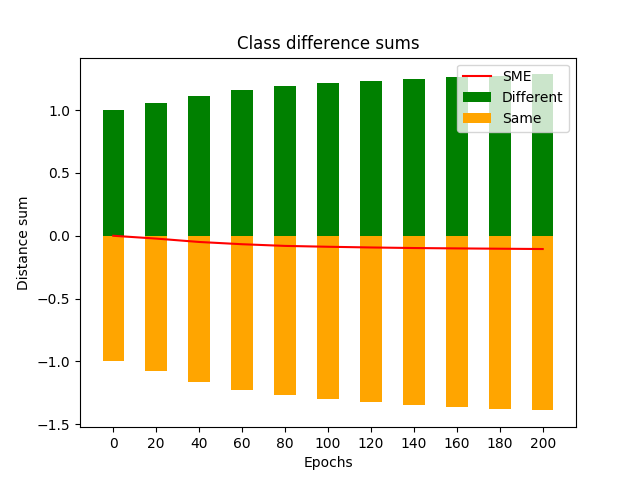
\includegraphics[width=1.\linewidth]{images/plotMethod_ClDiffSums_AIDS_E_GDL_18_23h-04m}
				\caption{SME decreasing {\footnotesize(Dataset \textit{AIDS})}}
				\label{fig:plotmethodcldiffsumsaidsegdl1823h-04mhe}
			\end{subfigure}
			\begin{subfigure}{0.45\textwidth}
				\centering
				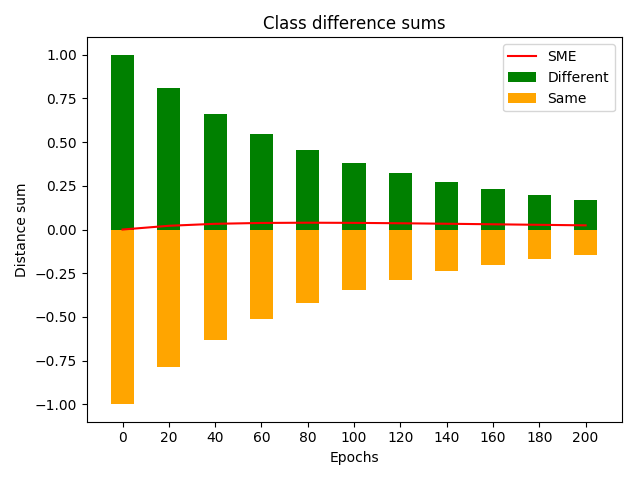
\includegraphics[width=1.\linewidth]{images/plotMethod_ClDiffSums_MSRC_9_E_GDL_22_00h-05mExp3}
				\caption{SME increasing {\footnotesize(Dataset \textit{MSRC\_9})}}
				\label{fig:plotmethodcldiffsumsmsrc9egdl2200h-05mexp3}
			\end{subfigure}
			\caption{SME error examples}
			\label{fig:SMEExamples}
		\end{figure}
	
		The two examples visualize a decreasing and thereby improving SME (\ref{fig:plotmethodcldiffsumsaidsegdl1823h-04mhe})
		and an increasing and thereby degenerating SME (\ref{fig:plotmethodcldiffsumsmsrc9egdl2200h-05mexp3}).
		Notice how the SME is decreasing, but the sum of the same cluster distances is increasing.
		Nevertheless, the decreasing SME states, that the different cluster distances are increasing faster.
		Similarly the SME is increasing, but the sum of the different cluster distances is decreasing, all be it slower than the decreasing of the same cluster distances.		

		\paragraph{Global, batch-wise and local interpretation}
		It is crucial to note, that the update rule (section \ref{subsec:EWL}) adjust the edge weights in the WLLT based on a \textit{local} evaluation of the edge weights at the time of the update.
		That is, the edge weight changes are defined using two graph samples each.
		Let us call the SME computed right after the definition of the edge weight adjustment for an individual pair of graphs in the batch the local SME.
		This local SME decreases compared to right before the definition of the edge weight adjustment every time, since the update rule is designed to do so.
		However, as described in section \ref{subsec:WLLT_ew_init}, the edge weight changes originating from comparing one pair of graphs may be changed (averaged) and are only applied after each epoch.
		Computing the SME at this point we call computing the batch-wise SME.
		It is no longer guaranteed that the SME decreases for all (hyper-)parameter settings.
		That is because changing one edge weight in the WLLT may influences the distance between several graphs, both from the same and from different classes.
		The same holds true for the global SME, which we defined first. 
		The first and most direct indicator for success of the l-WWLLT method is, to reduce this global SME.
		
		As mentioned before, we make use of additional evaluation methods.
		For example the classification accuracy using the l-WWLLT-kernel (section \ref{subsec:lWWLLTkernel}) in a support vector machine (section \ref{subsec:method_svm}), 
		or by measuring the quality of the given clusters of graph classes with respect to the similarity measure (section \ref{subsec:method_cl_eval}).
		Notice how these three evaluation methods measure different aspects of the defined similarity measure.
		After presenting these two other evaluation methods, the reasoning behind this evaluation strategy are summarized in section \ref{subsec:method_eval_strategy}.
		
	\subsubsection{Support Vector Machine} \label{subsec:method_svm}
	
		One of the easiest way to compare the performance of this learner to other methods with the similar goal to define a graph similarity measure, is to use a C-Support Vector machine (SVM)~\cite{1992_Boser_CONF, 2003_Hsu_CONF}.		
		SVMs try to define a model, which predicts target values (i.e. class labels) of features of given test data.		
		In essence, they map feature vectors with known target values (training data) into a higher (maybe infinite) dimensional space and find a linear separating hyperplane (or support vectors) with the maximal margin in this higher dimensional space.
		This hyperplane is then used for further classification decision on the test data~\cite{1992_Boser_CONF}. 
		Many researchers measure their implementations in the mean classification accuracy (and standard deviations) of a computed kernel in a $10$-fold cross validation SVM (for example \cite{2016_Kriege_NIPS, 2019_Schulz_CONF, 2011_Shervashidze_JMLR, 2020_Siglidis_CONF}) (repeated 10 times with random folds).
		That is, to partition the graph dataset in a training and evaluation set, and evaluate the performance of the computed support vectors on the training set.
		For better comparability, we use this method as well.
		
		To use a suitable SVM, the computed distance matrix is transformed into a kernel matrix using the definition of the Tree-sliced Wasserstein kernel (section \ref{subsec:lWWLLTkernel}).
		This is the main motivation to keep the edge weights positive, because this implies a positive definite kernel~\cite{2019_Le_NIPS}.
		It is recommended to scale the kernel linearly to the interval $[0,1]$.
		This scaling may reduce dominating effects of attributes with greater numeric range over those with smaller ones and it may avoid numerical difficulties during the calculation~\cite{2003_Hsu_CONF}.
		However using only non-negative distances, the kernel definition using the exponential function, and having distances of value zero on the diagonal of the distance matrix already lead to properly scaled values.
	
	\subsubsection{Cluster Evaluations} \label{subsec:method_cl_eval}
	
		In order to evaluate the already present clustering, when using the similarity measure induced by some (learned) edge weights $w$, we use the scores presented in section \ref{subsec:def_cl_scores}.
		Given the distance matrix of all graph classes according to the defined l-WWLLT-distance, no further parameters are required.
		To summarize, we use the Silhouette coefficient $S_{\text{SC}}$ to evaluate the tightness and separation of the cluster.
		An increasing Silhouette coefficient (possibly approximating $1.0$) is desirable in this application.
		We use the Davies-Bouldin score $S_{\text{DB}}$ to evaluate the similarity between the clusters.
		A decreasing Davies-Bouldin score is desirable in this application.
		We use the Calinski-Harabasz score $S_{\text{CH}}$ to evaluate the cluster dispersion.
		An increasing Calinski-Harabasz score is desirable in this application.
		
		Besides these scores, we track a multitude of other values with respect to the clustering.
		For example the maximum, minimum and mean distance between all samples the same and different classes, for all classes.
		We may refer to the distance between samples of the same class as intra-distance and to to the distance between samples of the different class as inter-distance.
		Notice that not all of these measurements have a fixed desired trajectory.
		Key indicators for an improved clustering are increasing minimum inter-distance, decreasing maximum intra-distance.
		
		As a visualization of the clustering a T-distributed Stochastic Neighbor Embedding (t-SNE)~\cite{2008_Maaten_CONF} was used\footnote{More specifically the default implementation from the package \texttt{sklearn.manifold.TSNE} on \url{https://scikit-learn.org/stable/modules/generated/sklearn.manifold.TSNE.html}.}. 
		These embeddings are able to visualize high-dimensional data by considering data point similarities as (low-dimensional) joint probabilities.
		They then try to minimize the Kullback-Leibler divergence between these.
		Note that the visualizations are not deterministic and can be visualized differently in multiple computations.
						
	\subsubsection{Method Evaluation Strategy} \label{subsec:method_eval_strategy}
	
		Measurements like the mentioned statistics of all computed distances or visualizations of the edge weights in the WLLT, the distance matrix, and the WLLT itself were used to guide the implementation and the understanding of the method.
		The experiments with the l-WWLLT method, and thus its success were guided by considering the SME, the accuracy of the implied kernel, and the implied scores of the graph clustering.		
		It is not mandatory for these three evaluations to align in their assessment. %LaterTODO: Find theoretical ideas for this
		However we assume, that if a distance matrix, reflects a clearer separation between the samples of different classes, also relates to a better accuracy of the SVM, since the optimal separating hyperplane (or support vectors) should be less faulty.
		This may be true for the other way as well. 
		Although a clear cluster separation does not improve all cluster scores equally.
			
		It is important to keep in mind, that in the training process and our experiments, the clustering is given by the dataset and not computed by the learner itself.
		We only measure that the graph structures, represented in the graph representations relates to the given graph classifications.
		This also means, that if the classifications do not relate to the WL-labels (unfolding trees), there may be little chance, that the computed weights in the WLLT can reflect the classifications at all.		
	
	\subsubsection{Comparison to Other Methods} \label{subsec:comparison_to_other_methods}
					
		After this explanation of the l-WWLLT method, we come back to the related work mentioned in section \ref{subsec:related_work} and compare this approach to similar ones.

		The researched method is similar to the WL-OA Kernel (see section \ref{subsec:def_WLOA}) but differs in an important aspect.
		While the WL-OA only considers the equal subset of WL-labelings between two graphs, our approach considers the complete comparison of all labels, and especially the differences.
		Our approach emphasizes the differences, since similarities between equal feature vectors of two graphs are reduced when computing their $L_1$-norm.
		The between different feature vectors remain when computing the $L_1$-norm.
		In other words, the WL-OA focuses on the paths of the WLLT from the root to the lowest common ancestors (WL-labels) which both graphs have in common~\cite{2016_Kriege_NIPS}.		
		Our method focuses on the part of the WLLT from the lowest common ancestor to the leaves, but considers both paths as well.
		This may seem more intuitive for the task of defining a dis-similarity measure, since all dis-similarities with respect to the WL-label representation are considered.
		Note, that unlike \citeauthor{2016_Kriege_NIPS} when proposing the WL-OA, we formulate the l-WWLLT with respect to categorical vertex labels only.
				
		As mentioned above, the Wasserstein distance depends greatly on its ground metric $d$.
		In different formulas for different Wasserstein distances given in section \ref{subsec:def_WassDist}, the ground metric is used either directly, to define the cost matrix or to define the used edge weights.						
		Using a tree metric as ground distance, allows us to use the efficient close formula definition presented in equation \ref{eq:TreeWassDist} in section \ref{subsec:def_WassDist}.
		\citeauthor{2019_Togninalli_NIPS} used the Wasserstein distance on a histogram like representation of graphs too~\cite{2019_Togninalli_NIPS}.
		But as ground metric they used the normalized Hamming distance (for categorical vertex features) or the Euclidean distance (for continuous vertex features).
		Therefore a key difference between their approach and the one presented in this thesis, is to define and alter the ground distance as a tree metric instead.		
		If the learning process can improve the overall performance of the similarity measure based on the tree metric, one may relate this performance to the performance when using the normalized Hamming distance or the Euclidean distance again.
		
		The graph representations used in the NoG Kernel by \citeauthor{2019_Schulz_CONF} only consider quantities of vertex and edge labels.
		Using a uniform edge weight initialization for the WLLT, this quantitative approach is included in the representation of the graph representation in the l-WWLLT (for the zeroth layer of the WLLT).
		One may argue, that the second layer in the WLLT holds similar information as the edge label count in the NoG.
		However we did not consider original edge labels.
		By including more layers, than just the zeroth, the l-WWLLT method includes structural information (on the neighborhoods and thus edges).
		Which differs from the NoG Kernel since it ignores structural information~\cite{2019_Schulz_CONF}.
		Note however, that depending on the dataset, the original vertex (and edge) labels themselves can contain structural information as well.
		For example in graph modeling molecular structures often include information on the used atoms in the vertex labels.
		Often, the definition of an atom relates to possible structural properties as well.
		
\section{Experiments} \label{sec:experiments}
	
	In this section the conducted experiments are motivated and presented.
	Therefore, we first present the graph datasets used for the l-WWLLT distance learning (section \ref{subsec:datasets}).
	Then the general setup of the implemented method is explained (section \ref{subsec:exp_setup}).
	We summarize the most important parameters, and how different settings were combined.
	Note that some parameters significantly change the behavior of the implemented method and are primarily used for the research on what specific approach may produce the desired results.
	Further note, that the number of parameters was to great, to allow for an extensive grid search.
	Instead, a few guiding experiments are presented (section \ref{subsec:experiments}).
	More evaluations can be found in the appendix (appendix \ref{Appendix:FurtherResults}).

	192 different experiments on 17 different datasets were conducted using the final implementation of the l-WWLLT method.
	Since at first suitable parameter configurations were unknown, many of these experiments are spot checks for some parameter configurations.
	No extensive gird search was performed for all parameter combinations.
	No reliable trend in performance could be discovered for all datasets.
	That is why in this section we consider sets of experiments and discuss their implications for the research on the l-WWLLT method.
	In section \ref{sec:results} the best results over all computations are briefly summarized and presented.
		
	\subsection{Datasets} \label{subsec:datasets}
		For the experiments, three major sources for datasets of classified graphs were used.
		The TUDataset~\cite{2020_Morris_CONF} and versions of its graph datasets~\cite{2019_Ivanov_CONF}\footnote{\url{https://github.com/nd7141/graph_datasets}}
		and the OGB dataset~\cite{2020_Hu_CONF}.
		The versions of the TUDataset are based on the research by \citeauthor{2019_Ivanov_CONF} and can be seen as a pre-processing of the TUDatasets.
		Since these dataset version have the same names as the original datasets in the TUDataset, we refer to them by adding \enquote{\_c} as a suffix to the original name (see for example table \ref{tab:BestSVM_results}).
		Sine the results between these different versions of the datasets did not reveal substantial insight on the l-WWLLT method with respect to the research question, we do not go into further detail about their construction here.
				
		All loaded datasets were pre-processed, to ensure equalized treatment between the different sources, and to discard not needed information.
		This includes the deletion of graphs without vertices (where the WL-labeling is not applicable) and adding uniform vertex labels, if none are present.
		Furthermore the practical implementation converts the graphs into a standardized format consisting of only a vertex set with vertex labels, and an edge set.
		Since these practical implementation choices do not effect the theoretical reasoning and the l-WWLLT method itself, we do not discuss them in detail in this thesis.
		
		\subsubsection{TU Dataset} \label{subsec:TUDataset}
			
			The increased need of benchmark graph classification datasets lead to the construction of a graph dataset collection at TU Dortmund~\cite{2016_Kersting_CONF, 2020_Morris_CONF}.
			We refer to these datasets as TUDatasets.
			\citeauthor{2021_Schulz_CONF} argued, that these datasets may not be sufficient to test graph classification datasets, since good classification accuracy can be achieved by discarding a lot of structural information on the graphs (recall section \ref{subsec:comparison_to_other_methods}).
			Furthermore these datasets contain only $200$ to $5,000$ graphs, which may be to small for meaningful tests of graph kernels on classification tasks~\cite{2021_Schulz_CONF}.
			See table \ref{tab:TUDataset_Stats} for more information on the datasets.\footnote{*The dataset \textit{Tox21\_AhR} is also called \textit{Tox21\_AhR\_training}.}.
			However, because these datasets have been used by many other researchers and allow for a faster test driven development of the l-WWLLT method, we also use them for to evaluate the method as well (for example \cite{2007_Wale_CONF, 2016_Kriege_NIPS, 2011_Shervashidze_JMLR, 2015_Yanardag_CONF, 2020_Siglidis_CONF, 2020_Dwivedi_CONF, 2021_Schulz_CONF}).
			
			\begin{table}[H]
				\centering
				\begin{tabular}{|l|l|l|l|l|l|}
					\hline
					\textbf{Dataset} & \textbf{Source} & \textbf{\#Graphs} & \textbf{\#Classes} & \textbf{Avg. $|V|$} & \textbf{Avg. $|E|$} \\ \hline
					\multicolumn{6}{|c|}{\textbf{Small molecules}} \\ \hline
					\textbf{AIDS} & ~\cite{2008_Riesen_CONF, URL_TUDataset_NCI} & 2000 & 2 & 15.69 & 16.20 \\ \hline
					\textbf{MUTAG} & ~\cite{1991_Debnath_CONF, 2012_Kriege_CONF} & 188 & 2 & 17.93 & 19.79 \\ \hline
					\textbf{NCI1} & ~\cite{2007_Wale_CONF, 2011_Shervashidze_JMLR} & 4110 & 2 & 29.87 & 32.30 \\ \hline
					\textbf{NCI109} & ~\cite{2007_Wale_CONF, 2011_Shervashidze_JMLR} & 4127 & 2 & 29.68 & 32.13 \\ \hline
					\textbf{PTC\_MR} & ~\cite{2001_Helma_CONF, 2012_Kriege_CONF} & 344 & 2 & 14.29 & 14.69 \\ \hline
					\textbf{Tox21\_AhR}* & ~\cite{URL_TUDataset_Tox21} & 8169 & 2 & 18.09 & 18.50 \\ \hline
					\multicolumn{6}{|c|}{\textbf{Bioinformatics}} \\ \hline
					\textbf{DD} & ~\cite{2011_Shervashidze_JMLR} & 1178 & 2 & 284.32 & 715.66 \\ \hline % \cite{2003_Dobson_CONF}
					\textbf{ENZYMES} & ~\cite{2005_Borgwardt_CONF} & 600 & 6 & 32.63 & 62.14 \\ \hline % 2004_Schomburg % https://academic.oup.com/nar/article/32/suppl_1/D431/2505276?login=true
					\textbf{PROTEINS} & ~\cite{2005_Borgwardt_CONF} & 1113 & 2 & 39.06 & 72.82 \\ \hline % , 2003_Dobson_CONF
					\multicolumn{6}{|c|}{\textbf{Computer vision}} \\ \hline
					\textbf{MSRC\_9} & ~\cite{2015_Neumann_SPRINGER} & 221 & 8 & 40.58 & 97.94 \\ \hline
					\textbf{MSRC\_21} & ~\cite{2015_Neumann_SPRINGER} & 563 & 20 & 77.52 & 198.32 \\ \hline
					\textbf{MSRC\_21C} & ~\cite{2015_Neumann_SPRINGER} & 209 & 20 & 40.28 & 96.60 \\ \hline
				\end{tabular}
				\caption{Statistics on some TUDatasets}\label{tab:TUDataset_Stats}
			\end{table}			

			The TUdatasets are based on different graphs representing different data structures.
			For example, the \textit{MUTAG} dataset contains 188 graphs, depicting chemical compounds.
			In this representation, explicit hydrogen atoms have been removed. 
			The (initial) vertex labels stand for example atoms like for Carbon (0), Nitrogen (1), Oxygen (2), Fluorine (3), Iodine (4), Chlorine (5) and Bromine (6).
			The edges labels indicate the bond type of either aromatic (0), single (1), double (2) or triple (3).
			The classifications in this dataset are made according to their mutagenic effect on a bacterium~\cite{1991_Debnath_CONF}.

			Note that most, but not all, of these datasets have two class labels and that datasets with high amounts of different class labels require bigger batch sizes in order to represent all classes equally.
			More information on the individual datasets can be found online.\footnote{TUDataset list \url{https://chrsmrrs.github.io/datasets/docs/datasets/}}
															
		\subsubsection{OGB Dataset} \label{subsec:OGB}
			
			As mentioned above, the TUDatasets may not be ideal to test graph classification kernels.
			Thus there is a high demand for graph datasets where the graph classification is highly dependent on the graph structure.			
			In 2020 \citeauthor{2020_Hu_CONF} presented the Open Graph Benchmark (OGB)~\cite{2020_Hu_CONF}.
			This collection includes large-scale datasets from different domains and for different applications, such as vertex, link, and graph property predictions.
			The datasets are grouped into datasets with small (100 thousand to 1 million vertices), medium (>1 million vertices) and large (on the order of 100 Mio. vertices or 1 billion edges) graphs~\cite{2020_Hu_CONF}.
					
			The datasets \textit{ogbg-molhiv} and \textit{ogbg-molpcba} were initially considered for experimentation.
			But their size of 41,127 and 437,929 graphs was to big (with respect to RAM storage) to experiment on various configuration settings.
			Notice that for the evaluation, the distance matrix (and kernel matrix) is computed for every learned and stored edge weight vector.
			It is possible to continue the evaluation on a fraction of the matrices, or fractions of the datasets.
			Instead, the experiments were focused on smaller datasets from this framework, in order to execute and learn from more experiments.
			The OGB collection provides ten smaller datasets from MoleculeNet~\cite{2018_Wu_CONF}.
			However of those, only the datasets \textit{ogbg-molbace} and \textit{ogbg-molbbbp} match the requirements of samples for binary (not multi-task) classifications.
									
			The leaderboard\footnote{\url{https://ogb.stanford.edu/docs/leader_graphprop/\#ogbg-molhiv}} of classification performance on these datasets is organized by ROC-AUC (Receiver Operating Characteristics-Area Under The Curve) scores.
			This quality measurement and evaluation process was not introduced to the implemented method for this thesis and thus the evaluation on these two datasets from the OGB collection was not compared to the state of the art.
			This decision is justified by the desire to avoid introducing yet another evaluation strategy and because these two datasets were loaded and pre-processed differently than how the OGB framework proposes it.			
			Instead, these datasets are used only to track the performance against the l-WWLLT metric at its initialization, as described in the research question (section \ref{subsec:research_question}). 
			
	\subsection{Set Up} \label{subsec:exp_setup}
	
		For all experiments a few parameter settings were kept fixed.
		One may very them in later research.
		These parameters are the update frequency, -score and -intensity.
		For all experiments, the \textbf{update frequency} is set to \enquote{epoch}, which means that the edge weights were updated after computing the mean weight change for all edges and all graphs in the batch of one epoch. 
		For all experiments the \textbf{update scope} is set to \enquote{All layers equal}, which means that all layers are treated equally. One may use this parameter to change the update intensity for individual layers individually.
		
		The implemented Edge Weight Learner (as explained in section \ref{subsec:EWL}) has a few more parameters, whose values were changed during the experimentation phase.	
		Starting with the \textbf{WLLT depth} $D$, which refers to the deepest layer of the WLLT whose edge weights are changed.
		If it is set to $D=2$ only the edge weights of the layers $0$, $1$ and $2$ are updated (and used to define the update).
		The \textbf{learning rate} $lr$ refers to an adjustment parameter, typical for machine learning (section \ref{subsec:EWL}).
		The \textbf{batch size} $bs$ is the percentage of graphs of the whole dataset that are used for adjusting the edge weights in one epoch.
		Notice that the actual set of graphs for each epoch is determined before all epochs, such that each class is represented almost equally.
		The \textbf{push factor} ($f_{\text{push}}$), \textbf{pull factor} ($f_{\text{pull}}$) and \textbf{Heaviest Earth Threshold} ($t_{\text{he}}$) refer to the same parameters explained in section \ref{subsec:EWL}.
		The flag \textbf{$w\in[0,2]$} (or $w\notin[0,2]$) indicates, if all edge weights were limited to the interval $[0, 2]$. 
		The motivation for this parameter is explained in section \ref{subsubsec:exp_WeightLimit}.
		Notice that this can be understood as an upper boundary ($w\le 2$), since the edge weights are always kept non-negative anyways.
					
		All experiments were implemented in Python 3.7.7.
		The few reported runtimes were measured using an Intel Core i5-8300 CPU at 2.30GHz with 16GB of RAM using a single processor only.
	
\subsection{Experiments} \label{subsec:experiments}
		
	First experiments were conduced to guide implementation choices and sha\-pe the evaluation process.
	This includes not only the evaluation with respect the proposed SVM and cluster scores, but also with respect to tracking and visualizing the computed edge weights and the resulting clustering.
	Most of these evaluations are used and presented in the next sections about the experiments.
	
	
	\subsubsection{Batch Size, WLLT Depth and Number of Epochs} \label{subsubsec:exp_eopchs}
	
		\paragraph{Batch Size} The number of epochs is closely related to the batch size in the sense that both parameters relate positively to the possibilities of introduced or removed weight in the WLLT.
		However the batch size goes quadratically into the runtime and thus should kept low if possible.
		Furthermore, the evaluation and the application of the weight updates is performed after batch, a smaller batch size allows for a finer evaluation.
		That is why in general the batch size was kept at 50 to 200 graphs ($1\%$-$30\%$) for the datasets, depending on the size of the dataset and sizes of the graph classes.
		Examples are presented in tabular \ref{tab:BestSVM_results}.
		
		\paragraph{WLLT Depth} The depth of the WLLT has a significant impact on the runtime (and on the required storage) as well.
		Although as discussed, the size of the WLLT has linear effect on the runtime, the WLLT depth may have exponential effect on the WLLT size and thus the runtime.
		That is because the amount of WL-labels increases drastically, depending on the dataset (recall figures \ref{fig:plotwlltl2e0aids2915h-25m} and \ref{fig:plotwlltmutagl2}).
		Table \ref{tab:WLLTsize} in the appendix (\ref{Asub:WLLTStatistics}) lists the WLLT size up to layer four for a selection of datasets.
		Figure \ref{fig:wlltstatsallds} visualizes this table.
		
		\begin{figure}[H]
			\centering
			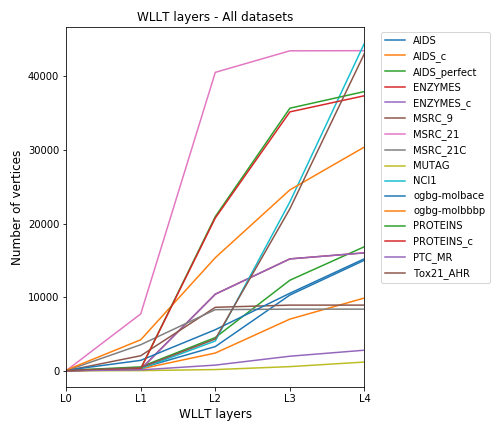
\includegraphics[width=0.7\linewidth]{images/WLLTstats_AllDs}
			\caption{Size of the WLLTs for various datasets.}
			\label{fig:wlltstatsallds}
		\end{figure}		
		
		Consider a graph representation of a graph $G$, and a WL-label $l$ which is a leaf in the WLLT and does not occur in the labelings for $G$.
		Since $l$ is present in the WLLT, it is present in the dataset and adding a next WLLT layer adds at least one child vertex to $l$.
		Depending on the depth and the dataset, $l$ may get many more children and all these do not occur in the labeling for $G$ as well.
		Thus notice, how higher layers imply a more sparse graph representation.
		After conducting some initial experiments with smaller datasets for WLLT depths of up to $10$, the WLLT depth was kept at $3$ or $4$.
		Higher layers do not seem to improve the resulting similarity measure significantly or at all.
		
		\paragraph{Number of Epochs} To determine how many epochs a learning algorithm should perform is usually related to the task of detecting over-fitting.
		For efficiency reasons, the evaluation and the learning procedure were separated, which is why an automatic detection of over-fitting was not implemented.
		Instead, the experiments were focused on collecting data for several parameter settings, and possibly detect over-fitting in hindsight.
		For a more granular evaluation the implementation saves intermediate results (a weight vector for the WLLT) every $10$-th epoch.
		
		The highest number of epochs was 1000.
		For the dataset \textit{AIDS} with 100 graphs per batch this took approximately 7.5 seconds per epoch (75 milliseconds per batch) and a total runtime of approximately two hours.
		The overall performance of the learned similarity measure did not show a clear relation (improvement or degeneration) with the number of epochs.
		Since all evaluations show noticeable development in the first $200$ epochs, this was used as the standard number of epochs for further experiments.
		See figure \ref{fig:plota1massevalscorecalinski} for example. 
		The visualized Calinski-Harabasz cluster score only changes significantly for the dataset \textit{PROTEINS\_c}.
		All other trajectories of the plots were maintained for most of the experiments for further learning epochs.
		No clear relation to other performance criteria (e.g. SVM accuracy or SME) of the l-WWLLT was detected.
		
		\begin{figure}[H]
			\centering
			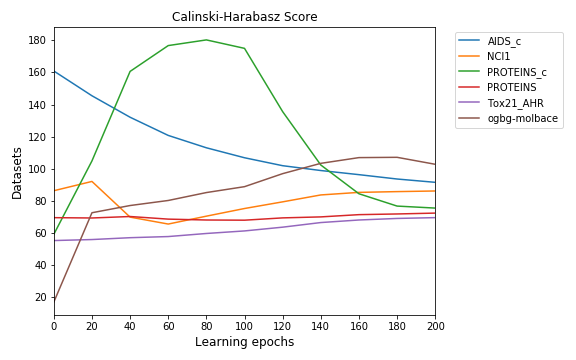
\includegraphics[width=\linewidth]{images/plotA1_MassCHS.png}
			\caption{Calinski-Score for several different datasets.}
			\label{fig:plota1massevalscorecalinski}
		\end{figure}
		
		The following plots for the dataset \textit{ogbg-molbace} are exemplary visualizations for this observation.
		They correspond to a run with learning epochs $e=500$, WLLT depth $D=5$, batch size of 100 graphs, learning rate $lr=1.0$ and push and pull factors of $0.2$ each with limited edge weight in the interval $[0,2]$ (figures \ref{fig:InterMeanMinMolBrace}, \ref{fig:IntraMeanMaxDistMolBace}, \ref{fig:plota1totalweightsumogbgmolbaceexp1}, \ref{fig:plota1scoresilhouetteogbgmolbaceexp1}, \ref{fig:plota1scoredaviesbouldinogbgmolbaceexp1}, \ref{fig:plota1scorecalinskiharabaszogbgmolbaceexp1}, and \ref{fig:plota1maxwplogbgmolbaceexp1}).
		
		\begin{figure}[!ht]
			\centering
			\begin{subfigure}{0.49\textwidth}
				\centering
				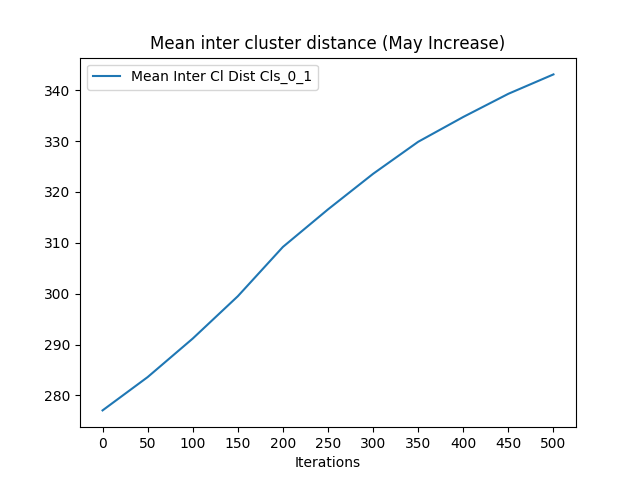
\includegraphics[width=1.1\linewidth]{images/plotA1_InterMeanClDist_ogbgMolbaceExp1}
				\caption{Mean cluster distance}
				\label{fig:plota1intermeancldistogbgmolbaceexp1-25m}
			\end{subfigure}
			\begin{subfigure}{0.49\textwidth}
				\centering
				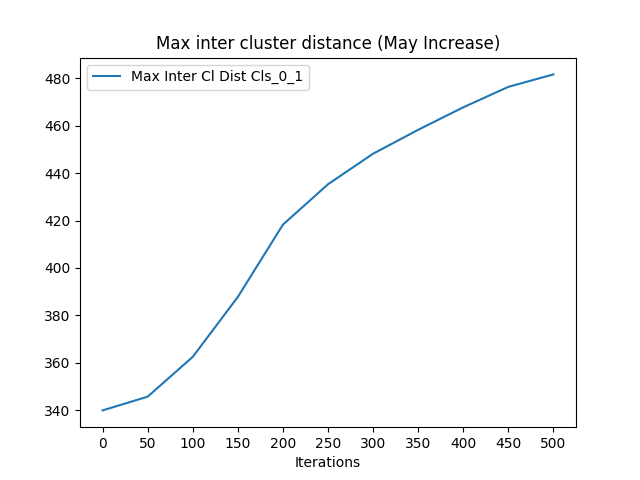
\includegraphics[width=1.0\linewidth]{images/plotA1_InterMaxClDist_ogbgMolbaceExp1}
				\caption{Maximum cluster distance}
				\label{fig:plota1intermaxcldistogbgmolbaceexp1}
			\end{subfigure}
			\caption{Mean and Maximum cluster distances - \textit{ogbg-molbace}}
			\label{fig:InterMeanMinMolBrace}
		\end{figure}
		
		The dataset \textit{ogbg-molbace} contains graphs, which are grouped into two clusters ($0$ and $1$).
		The two plots in figure \ref{fig:InterMeanMinMolBrace} show the mean and maximum distance between these classes (inter-distance).
		As desired, these distances increase over time.
		Round epoch 200, a slightly but rather insignificant reduced growth of the maximum distance can be noticed.		
		
		\begin{figure}[!ht]
			\centering
			\begin{subfigure}{0.49\textwidth}
				\centering
				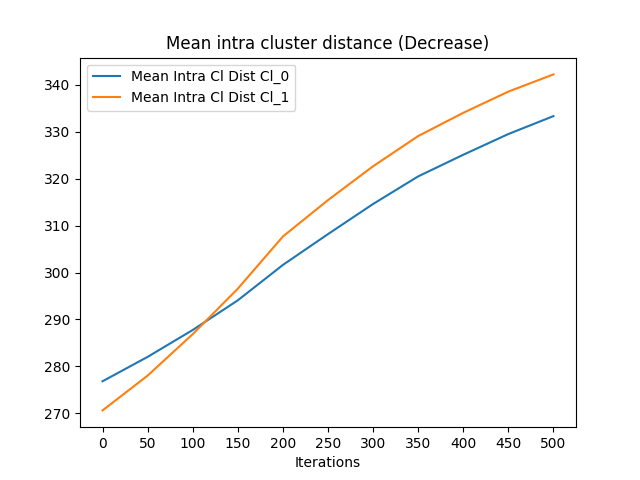
\includegraphics[width=1.1\linewidth]{images/plotA1_IntraMeanClDist_ogbgMolbaceExp1}
				\label{fig:plota1intrameancldistogbgmolbaceexp1}
			\end{subfigure}
			\begin{subfigure}{0.49\textwidth}
				\centering
				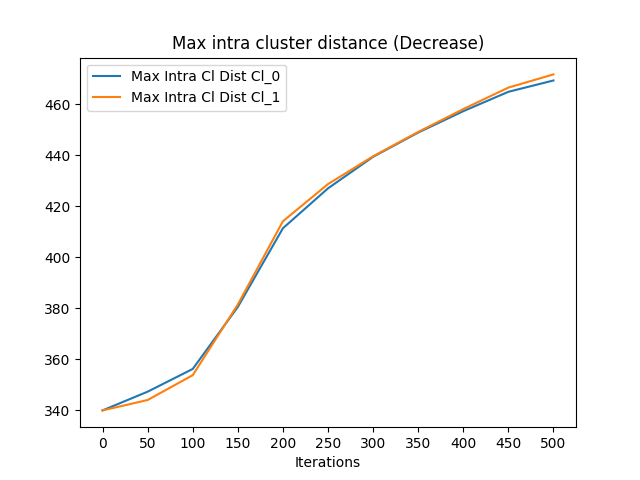
\includegraphics[width=1.1\linewidth]{images/plotA1_IntraMaxClDist_ogbgMolbaceExp1}
				\label{fig:plota1intramaxcldistogbgmolbaceexp1}
			\end{subfigure}
			\caption{Intra-cluster statistics - \textit{ogbg-molbace}}
			\label{fig:IntraMeanMaxDistMolBace}
		\end{figure}
		
		The two plots in figure \ref{fig:IntraMeanMaxDistMolBace} show the mean and maximum distance between samples of the same class each (intra-distance).
		Again around epoch 200, the reduced growth of the maximum distance can be noticed.
		One may as well describe it as a significant increase in the epochs 100 to 200.
		In contrast to the distances between different clusters however, the desired behavior would be decreasing intra-distances instead.
		Also notice that the order of magnitudes are equal to the inter-distances.
		
		\begin{figure}[H]
			\centering
			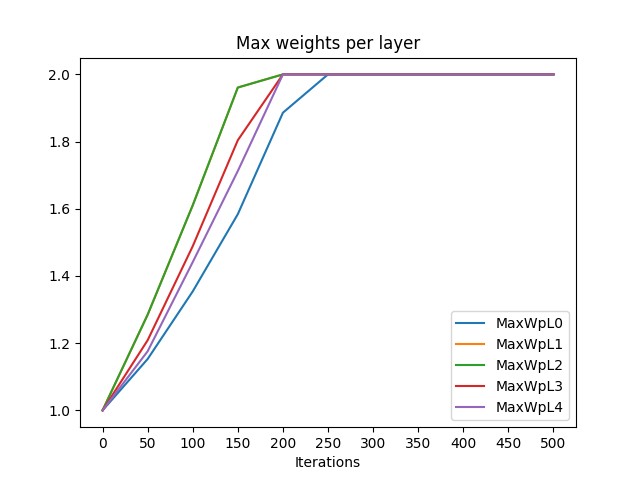
\includegraphics[width=0.7\linewidth]{images/plotA1_MaxWpL_ogbgMolbaceExp1}			
			\caption{Maximum weights per WLLT layer - \textit{ogbg-molbace}}
			\label{fig:plota1maxwplogbgmolbaceexp1}	
		\end{figure}
		
		The plot in figure \ref{fig:plota1maxwplogbgmolbaceexp1} gives a good explanation for the observed statistics up to epoch 200.
		It shows the maximum edge weights, to each of the five layers in the WLLT.
		Around epoch 200 the maximum edge weight for every epoch has reached the allowed limit, and stays there.
		Recall, that the update rule may treat weights of the same value equally.
		One may assume, that after epoch 200 more and more edge weights are set to the maximum of $2.0$ and no longer decreased.
		
		\begin{figure}[H]
			\centering
			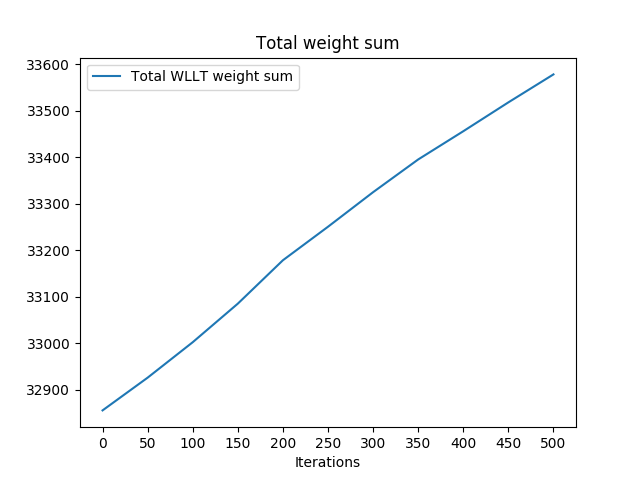
\includegraphics[width=0.7\linewidth]{images/plotA1_TotalWeightSum_ogbgMolbaceExp1}
			\caption{Total WLLT weight - \textit{ogbg-molbace}}
			\label{fig:plota1totalweightsumogbgmolbaceexp1}
		\end{figure}			
		
		These observations are supported by figure \ref{fig:plota1totalweightsumogbgmolbaceexp1}, which shows that the overall weight in the WLLT grows monotonically.
				
		\begin{figure}[H]
			\centering
			\begin{subfigure}{0.3\textwidth}
				\centering
				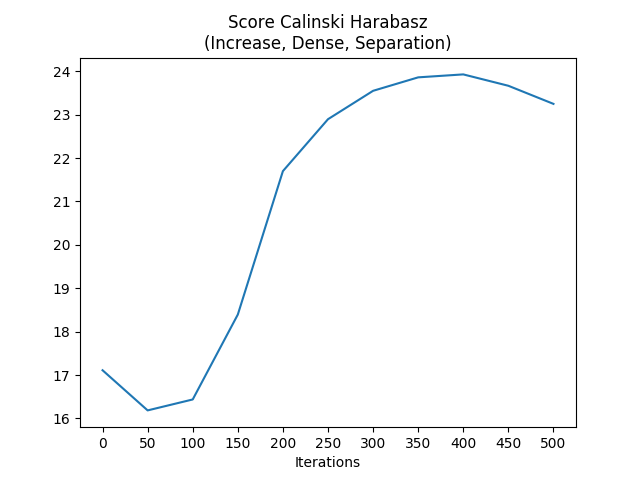
\includegraphics[width=1.1\linewidth]{images/plotA1_Score_Calinski_Harabasz_ogbgMolbaceExp1}
				\caption{CHS}
				\label{fig:plota1scorecalinskiharabaszogbgmolbaceexp1}
			\end{subfigure}		
			\begin{subfigure}{0.3\textwidth}
				\centering
				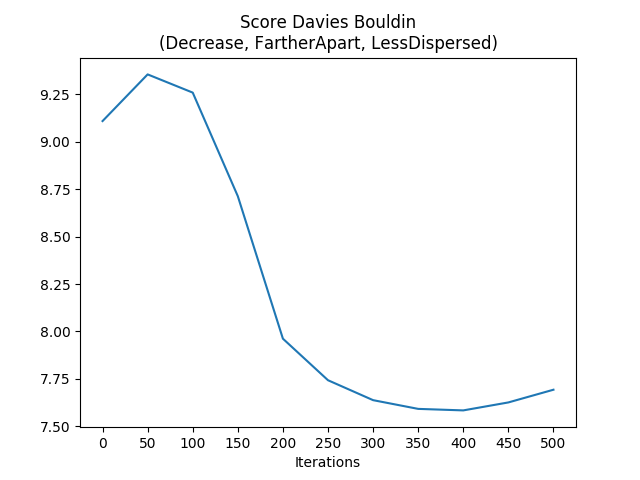
\includegraphics[width=1.1\linewidth]{images/plotA1_Score_Davies_Bouldin_ogbgMolbaceExp1}
				\caption{DBS}
				\label{fig:plota1scoredaviesbouldinogbgmolbaceexp1}
			\end{subfigure}
			\begin{subfigure}{0.3\textwidth}
				\centering
				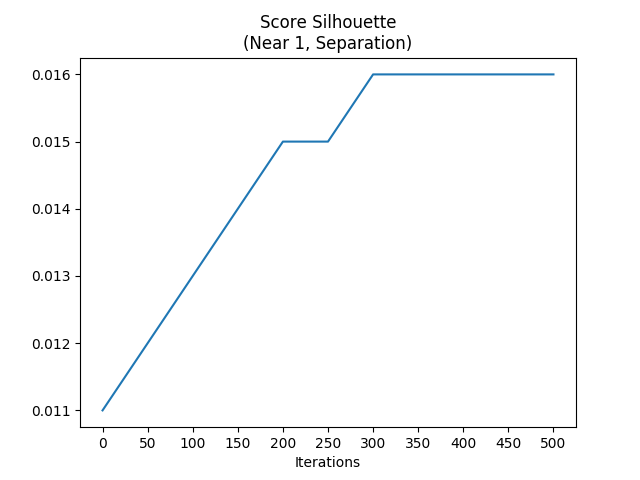
\includegraphics[width=1.1\linewidth]{images/plotA1_Score_Silhouette_ogbgMolbaceExp1}
				\caption{SS}
				\label{fig:plota1scoresilhouetteogbgmolbaceexp1}
			\end{subfigure}
			\caption{Cluster scores - \textit{ogbg-molbace}}
			\label{fig:ClScores_molbace}
		\end{figure}
				
		The cluster scores (see figures \ref{fig:ClScores_molbace}) indicate, that this edge weight maximum reduced the quality of the clustering.
		After epoch 200 all three scores indicate a reduced improvement and even degeneration.
		Recall, that the Calinski-Harabasz Score corresponds to the denseness of the clusters and their separation.
		Its improvement can be traced to the improved separation.
		The analogue situation can seen in the plot of the Davies-Bouldin score.
		The Silhouette Score stagnates after epoch 300 (at a low level).
		Since it corresponds to the separation, and not directly to the denseness of the clusters, one can deduce, that the degeneration of the other two scores can be explained by a degeneration of the cluster denseness.
		Combined with the insight from figure \ref{fig:plota1maxwplogbgmolbaceexp1} we can deduce, that the chosen setting leads to a reliable increase of the inter-distances, but not of the intra-distances and thus decreases the denseness of the clusters.
		
		\begin{figure}[H]
			\centering
			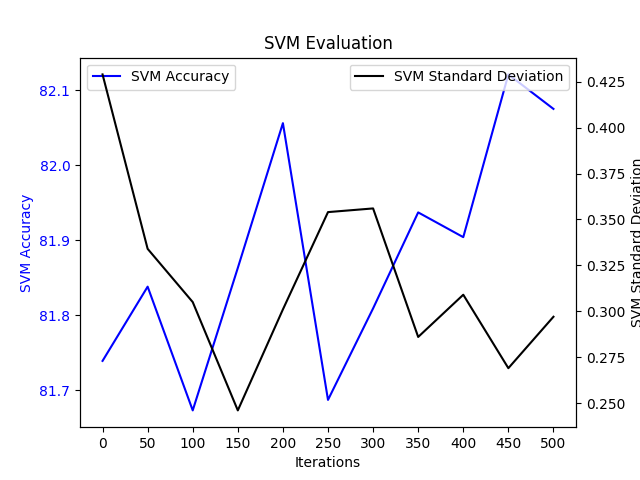
\includegraphics[width=0.7\linewidth]{images/plotA1_SVM_ogbgMolbaceExp1}
			\caption{SVM accuracy and standard deviation}
			\label{fig:plota1svmogbgmolbaceexp1}
		\end{figure}
		
		Interestingly, the SVM accuracies (shown in figure \ref{fig:plota1svmogbgmolbaceexp1}) do not obviously relate to the other plots.
		The SVM accuracy fluctuates at almost $82\%$.
	
	\subsubsection{Edge Weight Limit} \label{subsubsec:exp_WeightLimit}
		
		The initial configuration of the implemented learner did not include an edge weight limit.
		However the drawbacks of the multiplicative updates, in the context of the WLLT and the graph representations can be seen in the plots in figure \ref{fig:MUTAG_exponential_layers}.
		Each plot shows the edge weight distribution over all its WL-labels for all 500 learning epochs.
		The x-axes denote the WL-label (child to the considered edge), the y-axes the learning epoch and the z-axes the edge weights.
		The plots visualize how the (non-zero) development of most edge weights is overshadowed by an exponential growth of a few weights.
				
		\begin{figure}[H]
			\centering
			\begin{subfigure}{0.3\textwidth}
				\centering
				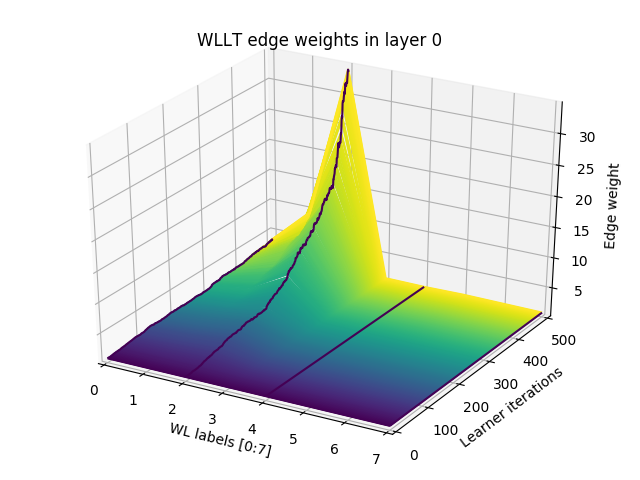
\includegraphics[width=1.\linewidth]{images/plotA3_WLLT_ewL0_MUTAG_d5_e500}
				\caption{Layer 0}
				\label{fig:fig:plota3wlltewl0mutagd5e500}
			\end{subfigure}		
			\begin{subfigure}{0.3\textwidth}
				\centering
				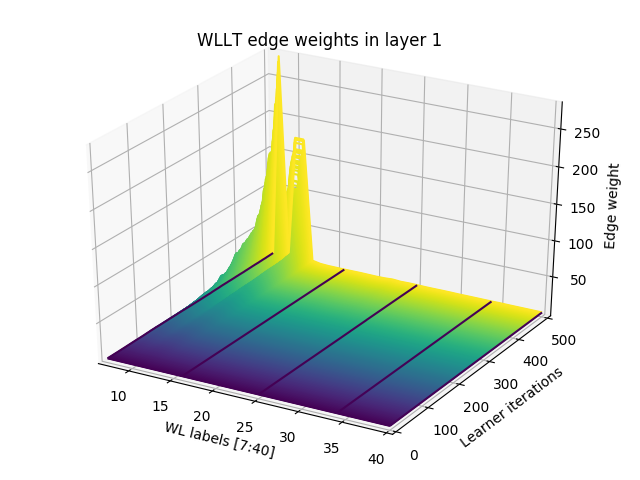
\includegraphics[width=1.\linewidth]{images/plotA3_WLLT_ewL1_MUTAG_d5_e500}
				\caption{Layer 1}
				\label{fig:fig:plota3wlltewl1mutagd5e500}
			\end{subfigure}
			\begin{subfigure}{0.3\textwidth}
				\centering
				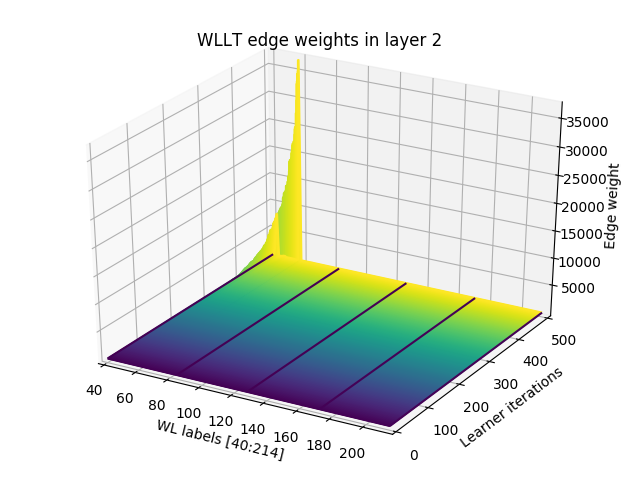
\includegraphics[width=1.\linewidth]{images/plotA3_WLLT_ewL2_MUTAG_d5_e500}
				\caption{Layer 2}
				\label{fig:fig:plota3wlltewl2mutagd5e500}
			\end{subfigure}
			\caption{Edge weights per WLLT layer - \textit{MUTAG}}
			\label{fig:MUTAG_exponential_layers}
		\end{figure}
	
		These and similar experiments show, that the same edge weights are updated predominantly in the same direction (mostly increased or mostly decreased).
		Thus by nature of the relative updates, some weights may increase exponentially.	
		A weight limit (to the interval $[0,2]$) was introduced in order to reduce this overshadowing effect and keep the edge weight values reasonable.
		The effect, that only a few edge weights are updated most frequently and strongly remains, and is discussed in the following paragraph.
			
		\paragraph{Redemption of unlimited Weights} The idea was, to limit the edge weights to the interval $[0, 2]$.
		As we can see in the descriptions of the other experiments, it was difficult to find a configuration for the implementation, such that the edge weights do not clip to the imposed ceiling and also do not vanish.
		Both results were observed.
		A grid search for the values $0.05$, $0.1$, $0.3$, $0.5$, $1.0$ was performed.
		While the learning rate varied between $1.0$, $0.9$ and $0.5$.
		No reliable improving configuration was found and the edge weight adjustment may have been to big throughout the grid search.
		This assumption can be supported by a rather positive result, when lifting the edge weight constraints on a learning setting with different parameters.		
				
		The plots in figure \ref{fig:MaxMeanWpL_AIDS} show how the maximum edge weight and the mean edge weight grow exponentially in the number of learning epochs.
		Similarly, the plots in figure \ref{fig:EWWireframe_AIDS} highlight the domination of individual edge weights in the layers $0$ and $1$.
		These wire-frame plots are a great tool to compare the development of all edge weights per layer.
		Noticeable in all experiments is, that in all layers, the total weight is concentrated on a small portion of WL-labels.
		These are the most common WL-labels and dominate the graph representations, especially in the lower layers.
		With each layer, the differentiation of the WLLT vertices (their WL-labels and thus the represented $k$-th neighborhoods) increases monotonically and the frequencies of all WL-labels decreases.
		Accordingly, the strength of the update rule on these WL-labels decreases.
		The domination of the weight of the \enquote{lowest edge} in figure \ref{fig:EWWireframe_AIDS} however, is unusually high, due to its exponential increase.
		
		\begin{figure}[H]
			\centering	
			\begin{subfigure}{0.45\textwidth}
				\centering
				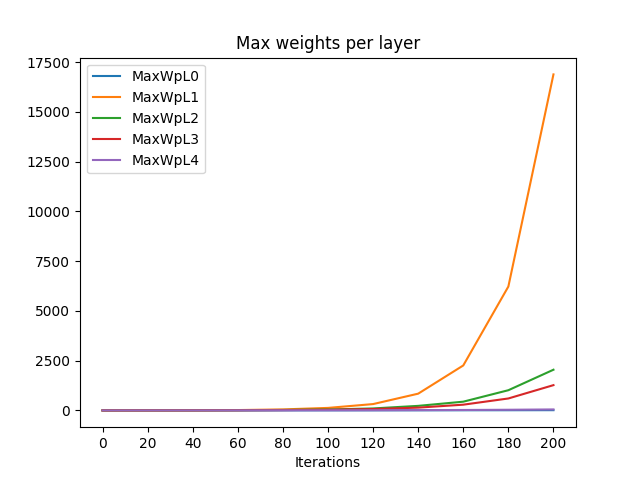
\includegraphics[width=1.1\linewidth]{images/plotA2_MaxWpL_AIDS_GDL_24_17h-05}
				\caption{MaxWpl}
				\label{fig:plota2maxwplaidsgdl2417h-05}
			\end{subfigure}
			\begin{subfigure}{0.45\textwidth}
				\centering
				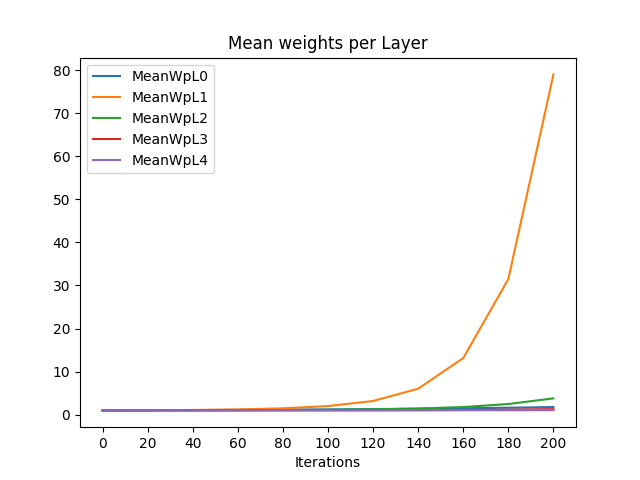
\includegraphics[width=1.1\linewidth]{images/plotA2_MeanWpL_AIDS_GDL_24_17h-05}
				\caption{MeanWpl}
				\label{fig:plota2meanwplaidsgdl2417h-05}
			\end{subfigure}
			\caption{Maximum and mean weights per layer - \textit{AIDS}}
			\label{fig:MaxMeanWpL_AIDS}
		\end{figure}
		
		
		\begin{figure}[H]
			\centering	
			\begin{subfigure}{0.45\textwidth}
				\centering
				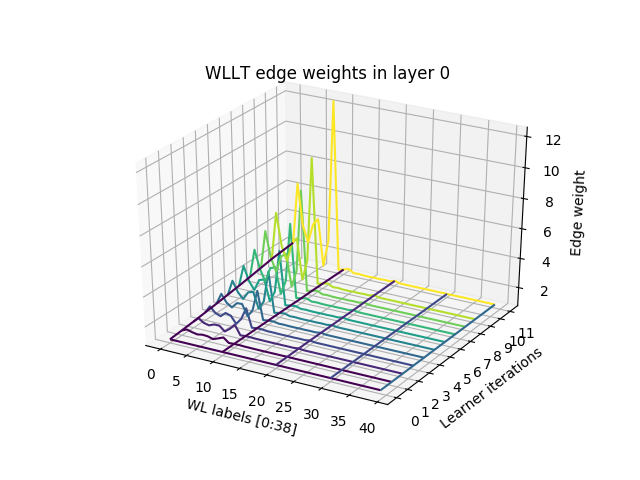
\includegraphics[width=1.1\linewidth]{images/plotA2_WLLTL0_AIDS_GDL_24_17h-05}
				\caption{Layer 0}
				\label{fig:plota2wlltl0aidsgdl2417h-05}
			\end{subfigure}
			\begin{subfigure}{0.45\textwidth}
				\centering
				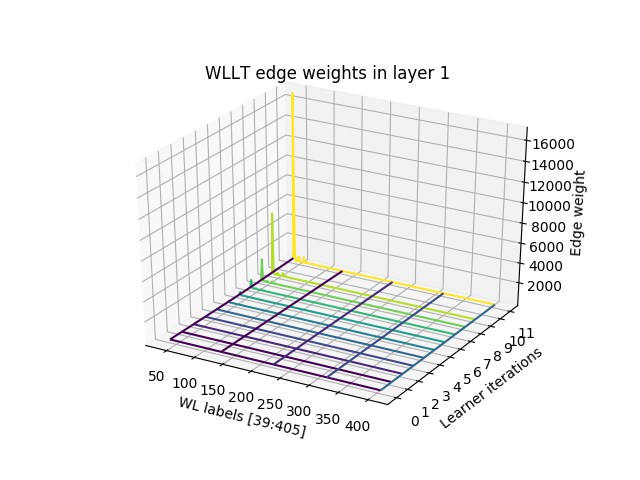
\includegraphics[width=1.1\linewidth]{images/plotA2_WLLTd1_AIDS_GDL_24_17h-05}
				\caption{Layer 1}
				\label{fig:plota2wlltd1aidsgdl2417h-05}
			\end{subfigure}
			\caption{Edge weights per layer, per iteration - \textit{AIDS}}
			\label{fig:EWWireframe_AIDS}
		\end{figure} 
		
		Despite this exponential edge weight increase, which was deemed undesirable in the early experiments, the evaluation shows how the SVM accuracy improves in this setting.
		The exponentially increasing total weight in the WLLT, shown in figure \ref{fig:plota2totalweightsumaidsgdl2417h-05} and the almost strictly monotonically improving SVM accuracy in figure \ref{fig:plota2svmaidsgdl2417h-05} indicate, that more research on different settings need to be considered.
		We also can conclude a positive answer of the research question from this result.
		However more experiments are required, do identify configuration strategy to obtain such improvements.
		
		\begin{figure}[H]
			\centering	
			\begin{subfigure}{0.45\textwidth}
				\centering
				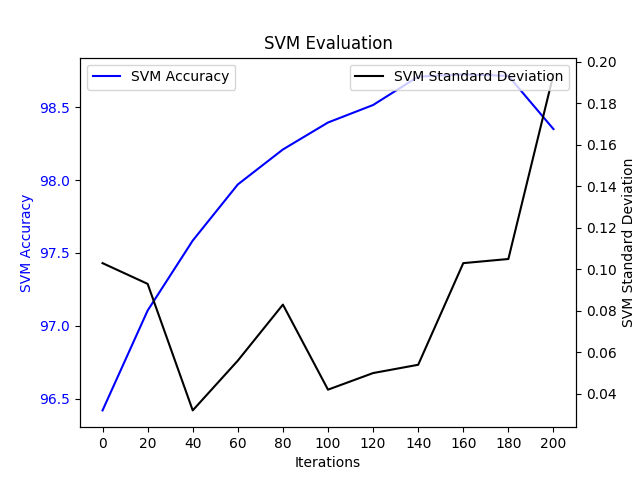
\includegraphics[width=1.1\linewidth]{images/plotA2_SVM_AIDS_GDL_24_17h-05}
				\caption{SVM}
				\label{fig:plota2svmaidsgdl2417h-05}
			\end{subfigure}
			\begin{subfigure}{0.45\textwidth}
				\centering
				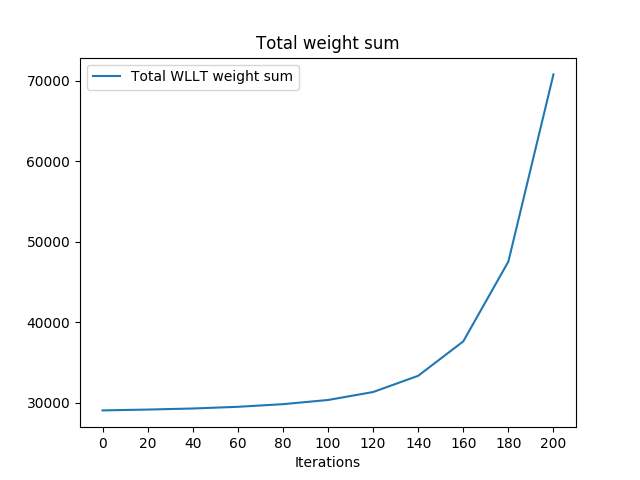
\includegraphics[width=1.1\linewidth]{images/plotA2_TotalWeightSum_AIDS_GDL_24_17h-05}
				\caption{Total weight sum}
				\label{fig:plota2totalweightsumaidsgdl2417h-05}
			\end{subfigure}
			\caption{SVM and total weight sum - \textit{AIDS}}
			\label{fig:SVMTotalWS_AIDS}
		\end{figure}	
	
	\subsubsection{Artificial Dataset} \label{subsubsec:exp_AIDS_perfect}
		
		To test the correctness of the implemented method an artificial dataset was created.
		This dataset shall represent a perfect separation of the classes with respect to the l-WWLLT with uniformly initialized edge weights.
		Therefore the 2000 graphs of the dataset \textbf{AIDS} were subdivided in class $A$, consisting of the first thousand graphs and class $B$, consisting of the second thousand graphs.
		On top of that, all occurring vertex labels for the graphs in class $B$ were changed to new vertex labels, which did not occur in class $A$.
		This implies, that the WLLT can be separated into tree vertices, representing WL-labels which occur in exactly one class as well.
		Even further, the set of original labels (in the first layer) can be separated into vertices belonging to graphs of exactly one class, and all WL-labels in its subtree belong to the same class.
		We refer to this artificial dataset as \textit{AIDS\_perfect}.
		
		Now notice, that the update rule still may increase and decrease all edge weights in both of these sets of subtrees.
		However we may expected that the edges in the first layer are increased more often (and more strongly) then all other edges over time.
		Note that, depending on the dataset, it is not trivial that the proposed update method behaves this way.

		The plots in figure \ref{fig:MeanMaxWpLAIDSperfect} refer to an execution with the settings $D=5$, $lr=1.0$, $bs=5\%$ (100 graphs), $f_{\text{pull}}=f_{\text{push}}=0.1$, $t_{\text{he}}=0.6$ and $w\in[0,2]$.
		Figure \ref{fig:plota0meanwplaidsperfectegdl0922h-03m} shows the average weights per WLLT layer (MeanWpL). 
		It is noticeable, how the average weight of the first layer increases more, than the one of the other layers.
		However this should be considered with the fact, that the other layers are much larger, and the graph representations contain lower values (normalized frequencies) for these WL-labels in general.
		Therefore it is more difficult to change their mean significantly during the learning procedure.
		Figure \ref{fig:plota0maxwplaidsperfectegdl0922h-03m} does not debunk the argumentation as well.
		It shows the maximum weights per layer (MaxWpL) and that these increase more rapidly in the lower layers.
				
		\begin{figure}[H]
			\centering
			\begin{subfigure}{0.45\textwidth}
				\centering
				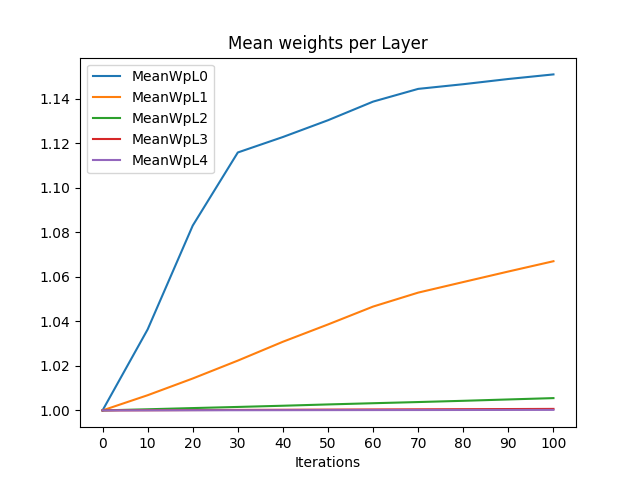
\includegraphics[width=1.1\linewidth]{images/plotA0_MeanWpL_AIDSPerfect_E_GDL_09_22h-03m}
				\caption{MeanWpL}
				\label{fig:plota0meanwplaidsperfectegdl0922h-03m}
			\end{subfigure}
			\begin{subfigure}{0.45\textwidth}
				\centering
				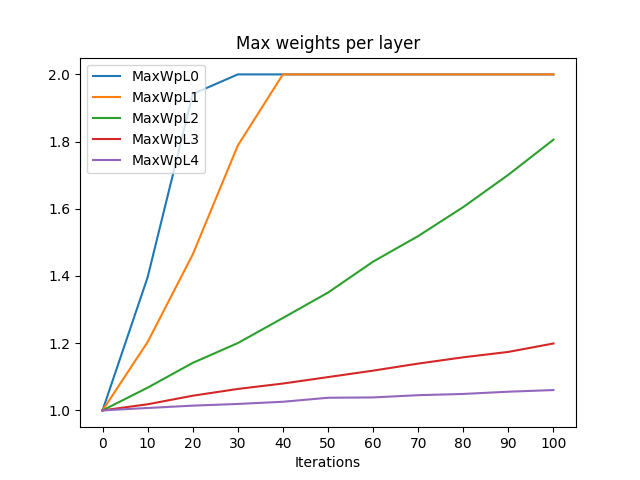
\includegraphics[width=1.1\linewidth]{images/plotA0_MaxWpL_AIDSPerfect_E_GDL_09_22h-03m}
				\caption{MaxWpL}
				\label{fig:plota0maxwplaidsperfectegdl0922h-03m}
			\end{subfigure}
			\caption{Mean and Maximum weight per layer - \textit{AIDS\_perfect}}
			\label{fig:MeanMaxWpLAIDSperfect}
		\end{figure}
	
		Notice how the limitation of the edge weights ($w\in[0,2]$) is visible in both graphs at around epoch $30$.
		In figure \ref{fig:plota0maxwplaidsperfectegdl0922h-03m} is visualized, how the maximum edge weights in the zeroth and first layer are no longer increased and stay at the maximum of $2.0$.
		In figure \ref{fig:plota0meanwplaidsperfectegdl0922h-03m} the growth of the average weights per layer is decreased afterwards.
		Recall, that the update rule allows to update edge weights with the same value in the same way.
		Thus these observations cannot be related to single edge weights in general.		
		
		The plots in figure \ref{fig:ClScoresAIDSperfect} show the evaluations on the Silhouette coefficient (SS), Davies-Bouldin score (DBS), and Calinski-Harabasz score (CHS).
		They reflect on the reached maximal edge weights as well.
		Up to epoch $20$ or $30$ they indicate an improvement. 
		After this, the cluster dispersion (caused by overall increasing weights) may be the reason for degenerating scores.
		
		\begin{figure}[H]
			\centering
			\begin{subfigure}{0.3\textwidth}
				\centering
				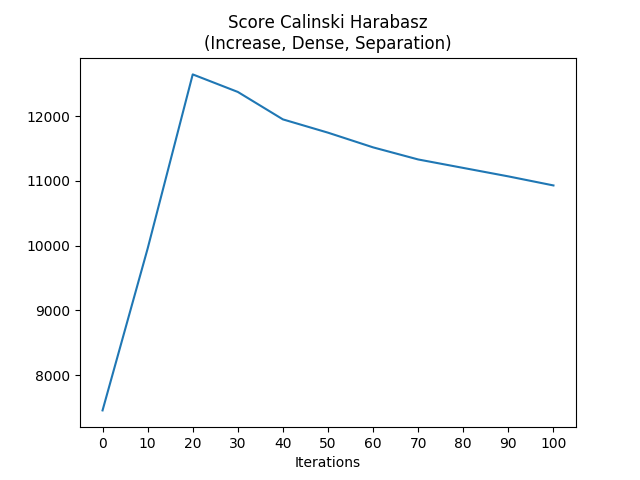
\includegraphics[width=1.1\linewidth]{images/plotA0_CHS_AIDSPerfect_E_GDL_09_22h-03m}
				\caption{CHS}
				\label{fig:plota0chsaidsperfectegdl0922h-03m}
			\end{subfigure}		
			\begin{subfigure}{0.3\textwidth}
				\centering
				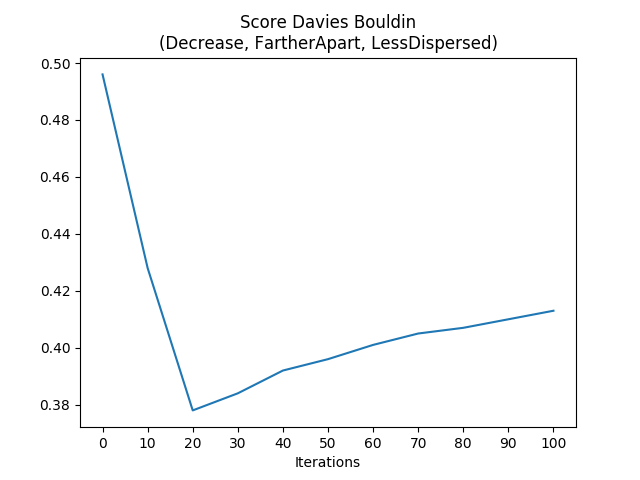
\includegraphics[width=1.1\linewidth]{images/plotA0_DBS_AIDSPerfect_E_GDL_09_22h-03m}
				\caption{DBS}
				\label{fig:plota0dbsaidsperfectegdl0922h-03m}
			\end{subfigure}
			\begin{subfigure}{0.3\textwidth}
				\centering
				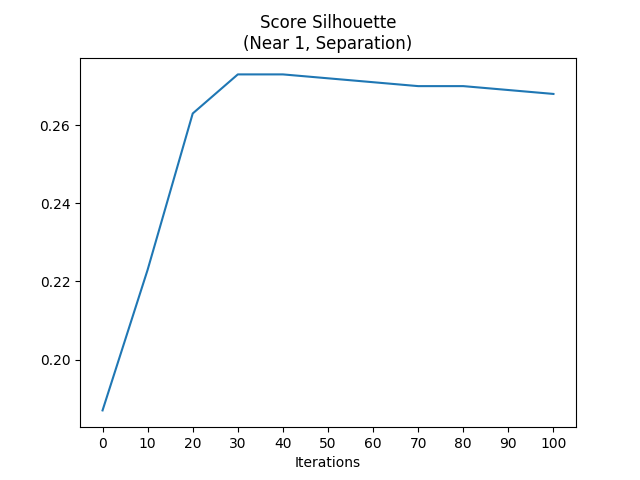
\includegraphics[width=1.1\linewidth]{images/plotA0_SS_AIDSPerfect_E_GDL_09_22h-03m}
				\caption{SS}
				\label{fig:plota0ssaidsperfectegdl0922h-03m}
			\end{subfigure}
			\caption{Cluster scores - \textit{AIDS\_perfect}}
			\label{fig:ClScoresAIDSperfect}
		\end{figure}
		
		A T-distributed Stochastic Neighbor Embedding (t-SNE)~\cite{2008_Maaten_CONF} visualizes the separation of the clusters in figure \ref{fig:TSNEAIDSperfect}.
		Overall, the clusters stay rather separated.
		An in- or decrease of the distance between them or the cluster denseness can not be noticed.
		However keep in mind, that the plots show a two-dimensional embedding of high dimensional (sparse) feature vectors.
		In this case, there are 34,296 WL-labels in the WLLT (with five layers $D=5$).
		Thus the feature vectors are 34,296-dimensional.
				
		\begin{figure}[H]
			\centering
			\begin{subfigure}{0.49\textwidth}
				\centering
				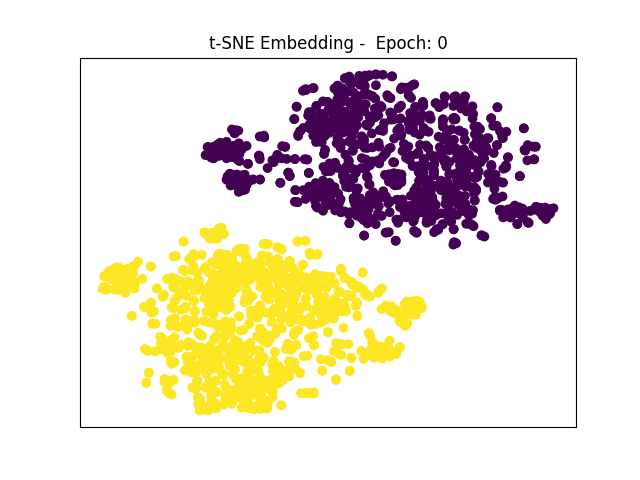
\includegraphics[width=1.1\linewidth]{images/plotA0_tSNE_e0_i0_AIDSPerfect_E_GDL_09_22h-03m}
				\caption{Epoch 0}
				\label{fig:plota0tsnee0i0aidsperfectegdl0922h-03m}
			\end{subfigure}
			\begin{subfigure}{0.49\textwidth}
				\centering
				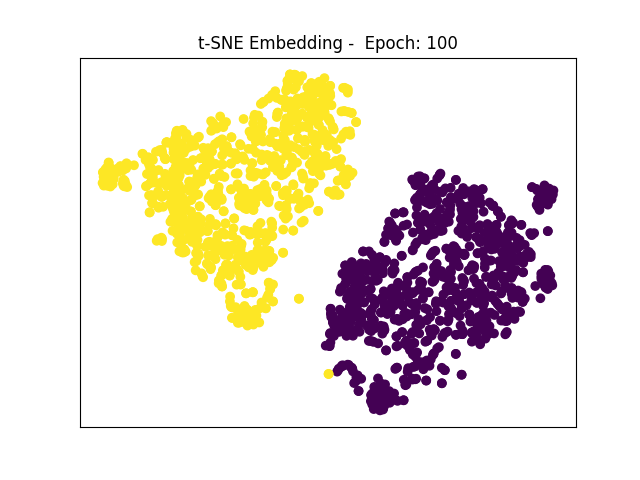
\includegraphics[width=1.1\linewidth]{images/plotA0_tSNE_e100_i10_AIDSPerfect_E_GDL_09_22h-03m}
				\caption{Epoch 100}
				\label{fig:plota0tsnee100i10aidsperfectegdl0922h-03m}
			\end{subfigure}
			\caption{T-SNE embeddings - \textit{AIDS\_perfect}}
			\label{fig:TSNEAIDSperfect}
		\end{figure}
		
		\begin{figure}[H]
			\centering
			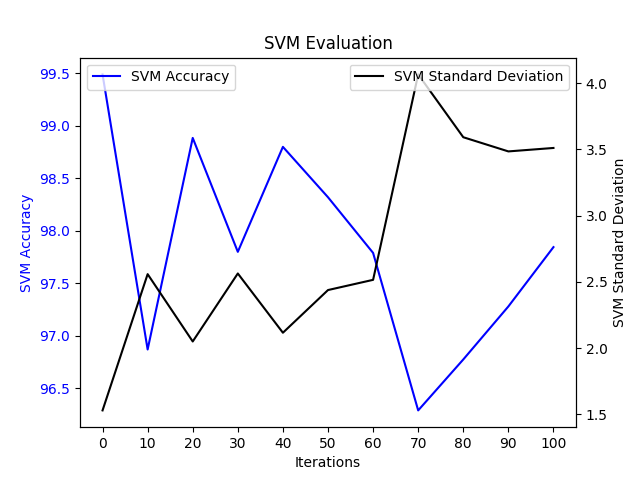
\includegraphics[width=0.7\linewidth]{images/plotA0_SVM_AIDSPerfect_E_GDL_09_22h-03m}
			\caption{SVM - \textit{AIDS\_perfect}}
			\label{fig:plota0svmaidsperfectegdl0922h-03m}
		\end{figure}		
	
		On the other hand figure \ref{fig:plota0svmaidsperfectegdl0922h-03m} illustrates that the SVM accuracy does not directly relate to these statistics.
		Overall, the SVM accuracy decreases and the best accuracy is reported for the initial state.
		This is indicates that the cluster scores and the SVM accuracy do not need improve or degenerate simultaneously.
		
		To summarize, this experiment supports the claim that the WLLT and the graph representations can be used in general to reflect a separation of graph clusters. 
		 	
	
	
	\subsubsection{Arbitrary Classifications} \label{subsubsec:exp_Arbitrary_Classifications} % Experiment 4
		In this experiment the learner was used two times with the same configuration.
		For one execution however, the classification for the graphs in the given dataset were randomized (keeping the number of classes). 
		The plots in figure \ref{fig:ArbitraryClCH} and \ref{fig:ArbitraryClSVM} show exemplary, that the learner behaves less predictable with respect to for example the CHS and the SVM accuracy.		
		Since the original classifications are related to the structures of the graph, but the randomized ones most likely not, this indicates that the learned edge weights do indeed capture information about the graph structures.
		
		\begin{figure}[H]
			\centering
			\begin{subfigure}{0.49\textwidth}
				\centering
				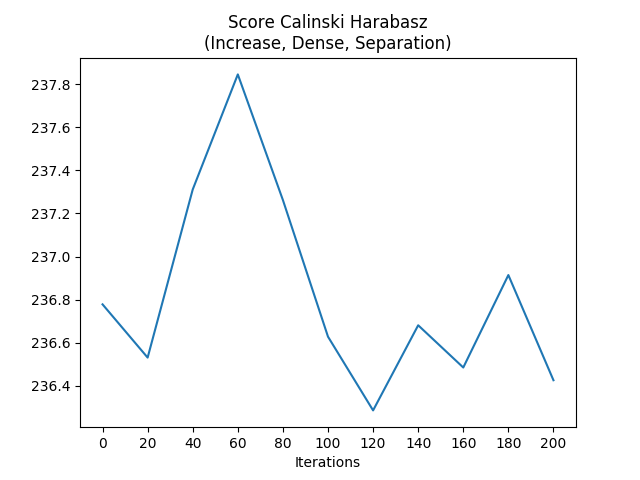
\includegraphics[width=1.1\linewidth]{images/plotE4_CH_E_GDL_09_16h-32m}
				\caption{Randomized classes}
				\label{fig:plote4chegdl0916h-32m}
			\end{subfigure}
			\begin{subfigure}{0.49\textwidth}
				\centering
				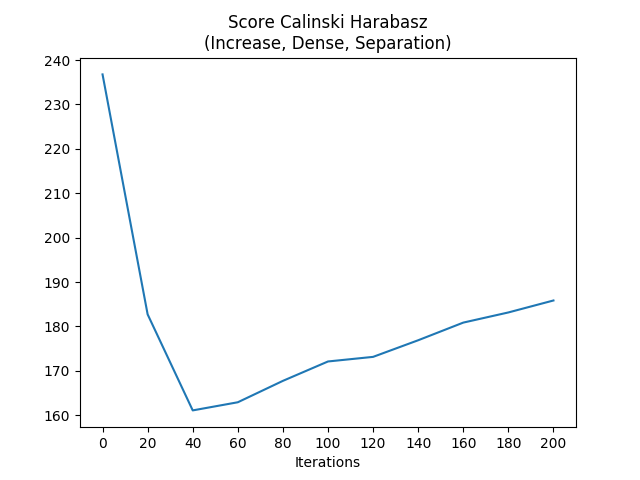
\includegraphics[width=1.1\linewidth]{images/plotE4_CH_E_GDL_09_17h-17m}
				\caption{Not randomized classes}
				\label{fig:plote4chegdl0917h-17m}
			\end{subfigure}
			\caption{CHS for the arbitrary classifications experiment - \textit{AIDS}}
			\label{fig:ArbitraryClCH}
		\end{figure}
		
		\begin{figure}[H]
			\centering
			\begin{subfigure}{0.49\textwidth}
				\centering
				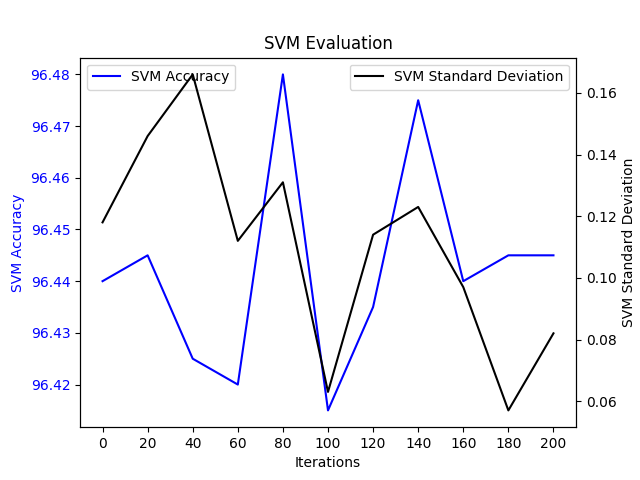
\includegraphics[width=1.1\linewidth]{images/plotE4_SVM_E_GDL_09_16h-32m}
				\caption{Randomized classes}
				\label{fig:fig:plote4svmegdl0916h-32m}
			\end{subfigure}
			\begin{subfigure}{0.49\textwidth}
				\centering
				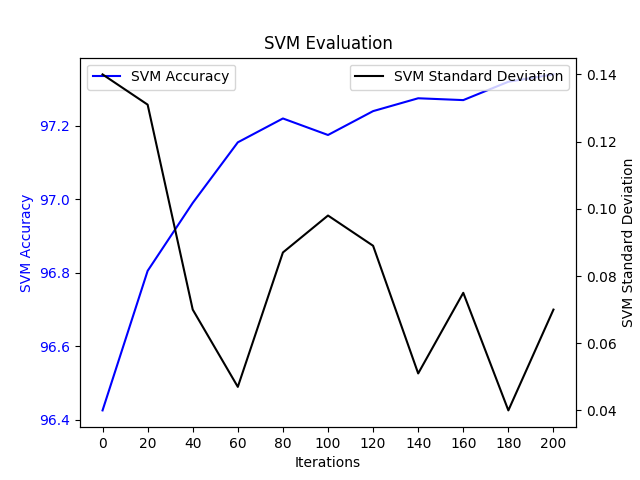
\includegraphics[width=1.1\linewidth]{images/plotE4_SVM_E_GDL_09_17h-17m}
				\caption{Not randomized classes}
				\label{fig:plote4svmegdl0917h-17m}
			\end{subfigure}
			\caption{SVM for the arbitrary classifications experiment - \textit{AIDS}}
			\label{fig:ArbitraryClSVM}
		\end{figure}
		
		Figure \ref{fig:WeightedWLLT} visualizes the WLLT with the learned edge weights.
		The plot in figure \ref{fig:plote4wlltl2e10gdl0917h-17mexp4} resembles a WLLT, typically for many of the conducted experiments.
		Plot \ref{fig:plote4wlltl2e10gdl0916h-32mexp4} on the other hand highlights how the learner has difficulties in defining meaningful weights for WL-labels and entire subtrees.
		
		\begin{figure}[H]
			\centering
			\begin{subfigure}{0.49\textwidth}
				\centering
				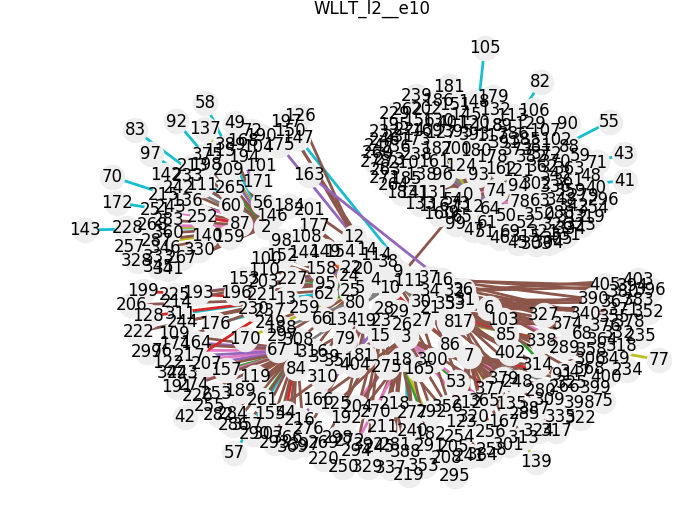
\includegraphics[width=1.1\linewidth]{images/plotE4_wllt_l2_e10_GDL_09_16h-32mExp4}
				\caption{Randomized classes}
				\label{fig:plote4wlltl2e10gdl0916h-32mexp4}
			\end{subfigure}
			\begin{subfigure}{0.49\textwidth}
				\centering
				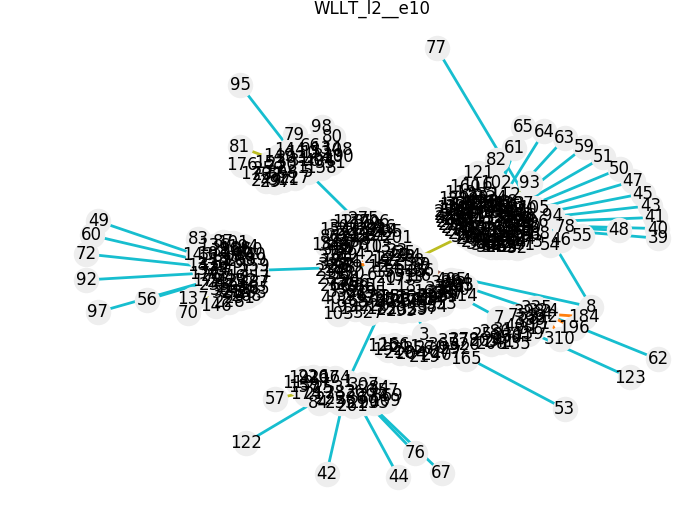
\includegraphics[width=1.1\linewidth]{images/plotE4_wllt_l2_e10_GDL_09_17h-17mExp4}
				\caption{Not randomized classes}
				\label{fig:plote4wlltl2e10gdl0917h-17mexp4}
			\end{subfigure}
			\caption{Weighted WLLT - \textit{AIDS}}
			\label{fig:WeightedWLLT}
		\end{figure}
	
		This experiment also indicates, that the l-WWLLT may not be able to learn arbitrary classifications in general.
		But this conclusion should be supported by more empirical or theoretical results.	

	\subsubsection{Relation between Pushing and Pulling} \label{subsubsec:exp_pp_factors}
		The success of the learning process seems to behave quite sensitively to the push and pull factors.
		This includes both their values and their relation between each other.
		Intuitively, if the pull factor is much greater than the push factor, the clusters collapse into each other and overlap.
		If on the other hand the push factor is much greater, the dispersion of the clusters increases which can lead to overlapping clusters as well.
		
		Researching the effect of these pp-factors and initializing them meaningfully becomes even more challenging, when different datasets are involved.
		Figure \ref{fig:plota4tsnee20enzymesgdl0418h} and \ref{fig:plota4tsnee0aids} show a t-SNE for the initialized l-WWLLT distances for the datasets \textit{ENZYMES} and \textit{AIDS} respectively.
		Notice how the different clusters overlap to different extends.
		
		\begin{figure}[H]
			\centering
			\begin{subfigure}{0.49\textwidth}
				\centering
				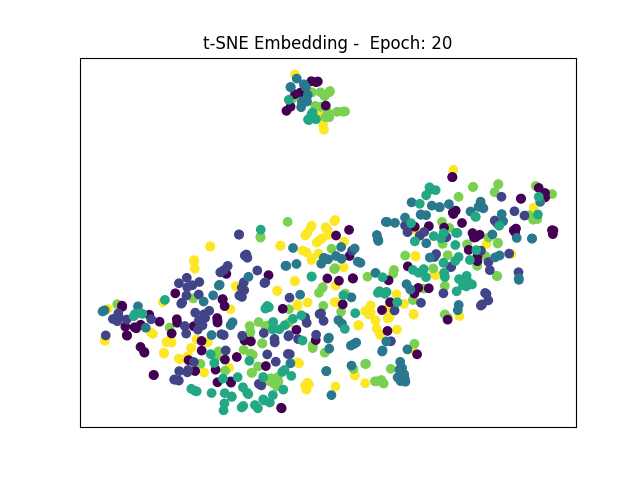
\includegraphics[width=1.1\linewidth]{images/plotA4_tSNE_e20_ENZYMES_GDL_04_18h-15m}
				\caption{\textit{ENZYMES}}
				\label{fig:plota4tsnee20enzymesgdl0418h}
			\end{subfigure}
			\begin{subfigure}{0.49\textwidth}
				\centering
				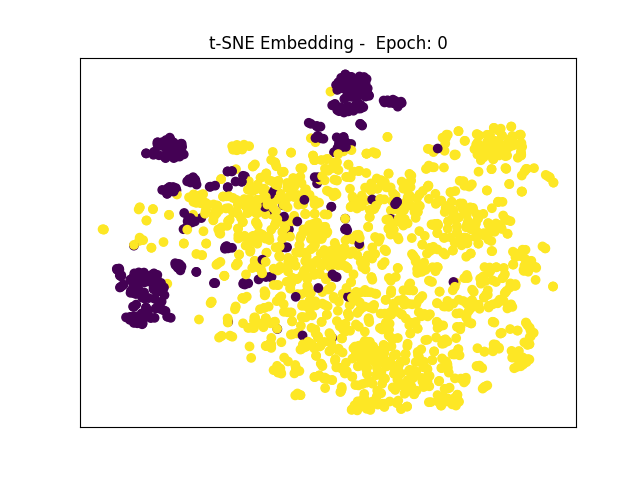
\includegraphics[width=1.1\linewidth]{images/plotA4_tSNE_e0_AIDS}
				\caption{\textit{AIDS}}
				\label{fig:plota4tsnee0aids}
			\end{subfigure}
			\caption{t-SNE of the uniformly initialized l-WWLLT}
			\label{fig:tSNE_init}
		\end{figure}
		
		The following four t-SNEs show the implied l-WWLLT distance after 100 learning epochs.
		In all configurations five WLLT layers were used.
		All except the first plot refer to the multiplicative update rule and a learning rate of $lr=1.0$.
		
		\begin{figure}[H]
			\centering
			\begin{subfigure}{0.49\textwidth}
				\centering
				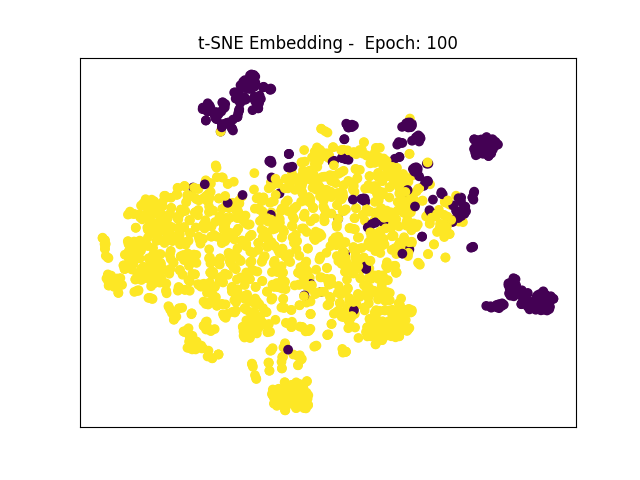
\includegraphics[width=1.1\linewidth]{images/plotA4_tSNE_e100_AIDS_E_GDL_18_23h-43m} % pp .3 lr .9
				\caption{pp-Factors: $0.3$, $lr=0.9$}
				\label{fig:plota4tsnee100aidsegdl1823h-43m}
			\end{subfigure}
			\begin{subfigure}{0.49\textwidth}
				\centering
				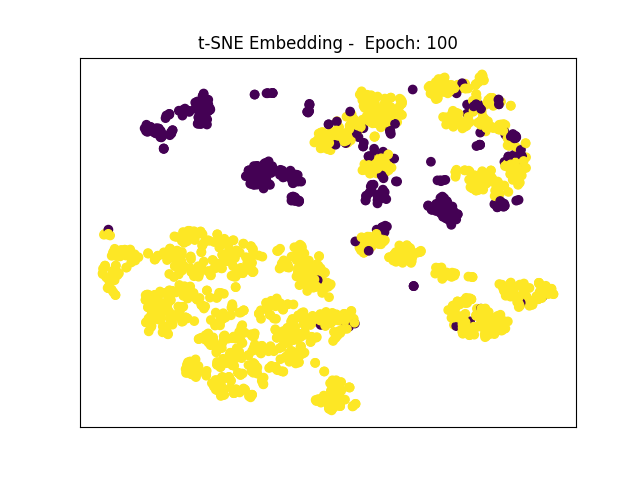
\includegraphics[width=1.1\linewidth]{images/plotA4_tSNE_e100_AIDS_E_GDL_24_17h-05m}  % pull.5push.5_noceil lr 1.0
				\caption{pp-Factors: $0.5$}
				\label{fig:plota4tsnee100aidsegdl2417h-05m}
			\end{subfigure}
			\caption{t-SNE of the l-WWLLT distances after $100$ epochs \& Equally strong push and pull factors - \textit{AIDS}}
			\label{fig:tSNE_100_A}
		\end{figure}
		
		Figure \ref{fig:plota4tsnee100aidsegdl1823h-43m} shows a configuration with $f_{\text{push}}=f_{\text{pull}}=0.3$ and $lr=0.9$.
		Almost no change to the initial state (figure \ref{fig:plota4tsnee0aids}) can be seen.
		One could argue that the clusters appear denser, but certainly not better separated.
		This may be, because the pp-factors, combined with the learning rate are to weak. 
		An example, where both are increased is shown in figure \ref{fig:plota4tsnee100aidsegdl2417h-05m}.
		Here the configuration $f_{\text{push}}=f_{\text{pull}}=0.5$ (and $lr=1.0$) was used.
		Again, the pp-factors are equally strong.
		Denser sub-clusters form in both clusters but the cluster separation remains weak.
		
		\begin{figure}[H]
			\centering
			\begin{subfigure}{0.49\textwidth}
				\centering
				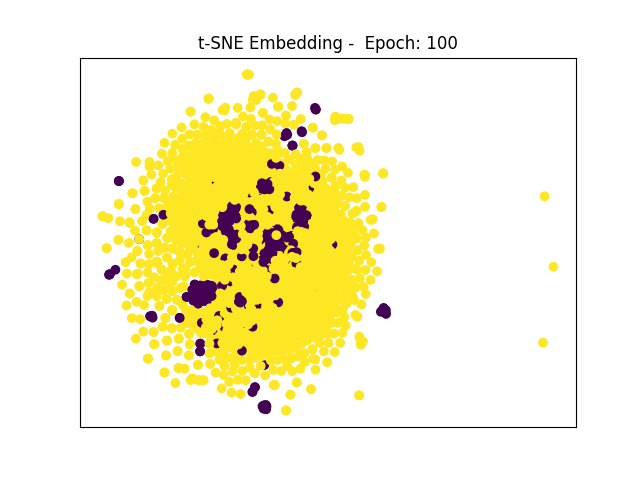
\includegraphics[width=1.1\linewidth]{images/plotA4_tSNE_e100_AIDS_E_GDL_24_12h-29m} % _pull.1 push.05 lr 1.0
				\caption{Pull: $0.1$, push: $0.05$}
				\label{fig:plota4tsnee100aidsegdl2412h-29m}
			\end{subfigure}
			\begin{subfigure}{0.49\textwidth}
				\centering
				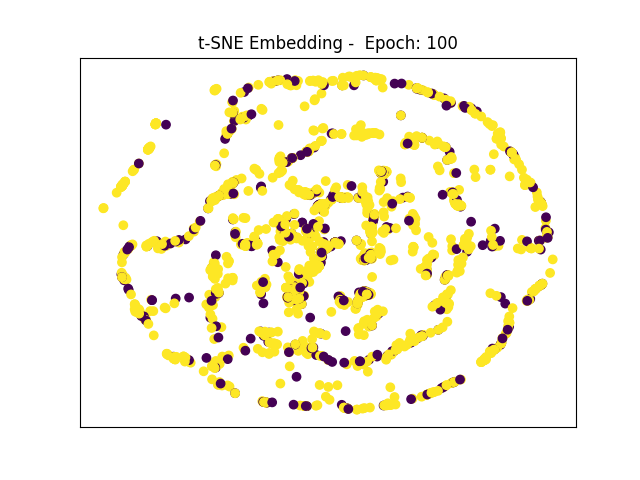
\includegraphics[width=1.1\linewidth]{images/plotA4_tSNE_e100_AIDS_E_GDL_24_13h-38m} % _pull.1 push.05 lr 1.0 absolute
				\caption{Pull: $0.1$, push: $0.05$ (additive update)}
				\label{fig:plota4tsnee100aidsegdl2413h-38m}
			\end{subfigure}
			\caption{t-SNE of the l-WWLLT distances after $100$ epochs \& Stronger pull. - \textit{AIDS}}
			\label{fig:tSNE_100_B}
		\end{figure}	
		
		Figure \ref{fig:plota4tsnee100aidsegdl2412h-29m} shows a configuration with unequal push and pull factors. 
		It is $f_{\text{push}}=0.05$ and $f_{\text{pull}}=0.1$.
		This is a good example for a typical case of heavily overlapping clusters because the pull factor is stronger that the push factor.
		
		Figure \ref{fig:plota4tsnee100aidsegdl2413h-38m} shows a configuration with $f_{\text{push}}=0.05$ and $f_{\text{pull}}=0.1$.
		Furthermore here, the pp-factors are used in the additive update rule.
		Interestingly the pull factor seems to pull again samples from both the same and different clusters together (compare to figure \ref{fig:plota4tsnee100aidsegdl2412h-29m}).
		However a significant separation is visible place at well.
		But such that the different clusters are separated.
		
		\begin{figure}[H]
			\centering
			\begin{subfigure}{0.49\textwidth}
				\centering
				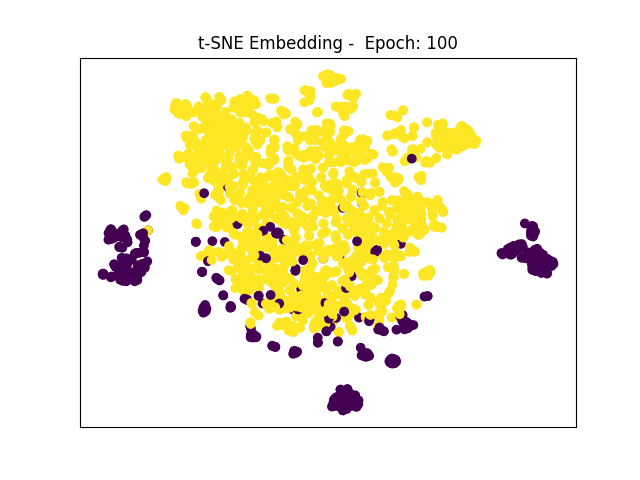
\includegraphics[width=1.1\linewidth]{images/plotA4_tSNE_e100_AIDS_E_GDL_09_01h_00m} %push 0.2 pull 0.1
				\caption{Pull: $0.1$, push: $0.2$}
				\label{fig:plota4tsnee100aidsegdl0901h00m}
			\end{subfigure}
			\begin{subfigure}{0.49\textwidth}
				\centering
				\includegraphics[width=1.1\linewidth]{images/plotA4_tSNE_e100_AIDS_E_GDL_03_02h-53m} %pull.1_psh.3
				\caption{Pull: $0.1$, push: $0.3$}
				\label{fig:plota4tsnee100aidsegdl0302h-53m}
			\end{subfigure}
			\caption{t-SNE of the l-WWLLT distances after $100$ epochs \& Stronger push - \textit{AIDS}}
			\label{fig:tSNE_100_C}
		\end{figure}
		
		Experiments, where the push factor is bigger than the pull factor tended to look like the original configuration, similar to figure \ref{fig:plota4tsnee100aidsegdl1823h-43m}
		again.
		Two examples of a common configuration from within a grid-search on the pp-Factors are visualized in figure \ref{fig:tSNE_100_C}.
		
		These exemplary plots do not cover the whole spectrum of the performed grid search. 
		But they shall give an insight on how different settings were perceived and that no clear trend could be established.
		Neither for all datasets, nor for one specifically.
		For further investigation, a more comprehensive grid search for the combination between pp-factors (and the learning rate) should be informative.	
	
	
%	\subsubsection{Single Layer Training} \label{subsubsec:exp_single_layer_training} % Experiment 5
%		The implementation allows to update edge weights of different layers differently.
%		So far, the other experiments do not motivate to use this.
%		For experimental variety however, a couple of experiments were conduced, such that only the edge weights of a single layer in the WLLT were updated.
%		Spot checks for different datasets and different WL layers did not show promising results.
%		While it was still possible to improve the cluster scores, the SVM performances were far behind the ones when updating all layers equally.
%		
%		%TODO: CONTINUE Exp5 of NCI1 or others. Plot where only one weight changes. Or delete this section.
%		
%		One may deduce from this, that the similarity of the graphs should be expressed as a matter of substructures of different sizes.
%		Since the WL-labels in layer $i$ only correspond to the i-1-th neighborhoods.
%		Adjusting the edge weights in different layers may allow to distinguish more accurately between variations in substructures of different sizes, which are relevant for the classification.
		
		
	\subsubsection{Dynamic PP-Factors} \label{subsubsec:exp_dynamic_pp} % Experiment 3
		So far all experiments are based on a fixed parameter configuration for all learning epochs.
		It is however a reasonable strategy, to dynamically change some of these parameters.
		For example by decreasing or increasing the learning rate, depending on the behavior of the error function.
		As mentioned before, the learning procedure is based purely on the local SME and does not consider the more expensive evaluations which were made after all learning epochs were completed.
		
		To investigate the effect of changing parameters, and to support the effectiveness of the implemented method, a set of experiments is based on the idea of continuing a given set of learning epochs with new learning parameters.
		We now consider a visually pleasing example on the dataset \textit{MSRC\_9}.
		400 learning epochs with parameters $D=4$, $lr=1.0$, $bs=0.3$, and $w\in[0,2]$ were performed.
		The first 200 epochs with a stronger pull, with $f_{\text{push}}=0.05$, $f_{\text{pull}}=0.3$.
		And the second 200 epochs with a stronger push, with $f_{\text{push}}=0.3$, $f_{\text{pull}}=0.05$.
		
		\begin{figure}[!ht]
			\centering
			\begin{subfigure}{0.49\textwidth}
				\centering
				\includegraphics[width=1.1\linewidth]{images/plotE6_CHS_MSRC_9_E_GDL_22_00h-05mExp3pull}
				\caption{First 200 epochs}
				\label{fig:plote6chsmsrc9egdl2200h-05mexp3pull}
			\end{subfigure}
			\begin{subfigure}{0.49\textwidth}
				\centering
				\includegraphics[width=1.1\linewidth]{images/plotE6_CHS_MSRC_9_E_GDL_22_00h-05mExp3pullpush}
				\caption{Second 200 epochs}
				\label{fig:plote6chsmsrc9egdl2200h-05mexp3pullpush}
			\end{subfigure}
			\caption{CHS - \textit{MSRC\_9}}
			\label{fig:E6CHS}
		\end{figure}
	
		\begin{figure}[!ht]
			\centering
			\begin{subfigure}{0.49\textwidth}
				\centering
				\includegraphics[width=1.1\linewidth]{images/plotE6_DBS_MSRC_9_E_GDL_22_00h-05mExp3pull}
				\caption{First 200 epochs}
				\label{fig:plote6dbsmsrc9egdl2200h-05mexp3pull}
			\end{subfigure}
			\begin{subfigure}{0.49\textwidth}
				\centering
				\includegraphics[width=1.1\linewidth]{images/plotE6_DBS_MSRC_9_E_GDL_22_00h-05mExp3pullpush}
				\caption{Second 200 epochs}
				\label{fig:plote6dbsmsrc9egdl2200h-05mexp3pullpush}
			\end{subfigure}
			\caption{DBS - \textit{MSRC\_9}}
			\label{fig:E6DBS}
		\end{figure}
	
		\begin{figure}[!ht]
			\centering
			\begin{subfigure}{0.49\textwidth}
				\centering
				\includegraphics[width=1.1\linewidth]{images/plotE6_SS_MSRC_9_E_GDL_22_00h-05mExp3pull}
				\caption{First 200 epochs}
				\label{fig:plote6ssmsrc9egdl2200h-05mexp3pull}
			\end{subfigure}
			\begin{subfigure}{0.49\textwidth}
				\centering
				\includegraphics[width=1.1\linewidth]{images/plotE6_SS_MSRC_9_E_GDL_22_00h-05mExp3pullpush}
				\caption{Second 200 epochs}
				\label{fig:plote6ssmsrc9egdl2200h-05mexp3pullpush}
			\end{subfigure}
			\caption{SS - \textit{MSRC\_9}}
			\label{fig:E6SS}
		\end{figure}
	
		Figures \ref{fig:E6CHS}, \ref{fig:E6DBS} and \ref{fig:E6SS} clearly show, how the cluster scores are degenerating in the first 200 epochs, and improving in the last 200  epochs (or the last 180 in case of CHS).
		Figure \ref{fig:E6SVM} Shows the same behavior with respect to the SVM accuracy.
				
		\begin{figure}[!ht]
			\centering
			\begin{subfigure}{0.49\textwidth}
				\centering
				\includegraphics[width=1.1\linewidth]{images/plotE6_SVM_MSRC_9_E_GDL_22_00h-05mExp3pull}
				\caption{First 200 epochs}
				\label{fig:plote6svmmsrc9egdl2200h-05mexp3pull}
			\end{subfigure}
			\begin{subfigure}{0.49\textwidth}
				\centering
				\includegraphics[width=1.1\linewidth]{images/plotE6_SVM_MSRC_9_E_GDL_22_00h-05mExp3pullpush}
				\caption{Second 200 epochs}
				\label{fig:plote6svmmsrc9egdl2200h-05mexp3pullpush}
			\end{subfigure}
			\caption{SVM - \textit{MSRC\_9}}
			\label{fig:E6SVM}
		\end{figure}
		
		The t-SNEs in figure \ref{fig:E6tSNE1} and \ref{fig:E6tSNE2} support these findings too.
		Notice, that the uniform initialization of the WLLT edge weights already allows for a good SVM accuracy (figure \ref{fig:plote6svmmsrc9egdl2200h-05mexp3pull}) and dense, clearly separated clusters in the t-SNE (figure \ref{fig:plote6tsnee0msrc9egdl2200h-05mexp3pull}).
		The figures \ref{fig:plote6tsnee40msrc9egdl2200h-05mexp3pull} and \ref{fig:plote6tsnee100msrc9egdl2200h-05mexp3pull} are clear visualizations for the effects of the non-intuitive effects of a strong pull factor.
		The embeddings are clearly degenerating and same class samples are pushed apart, or at least the distances between all samples become less pronounced.
		On the other hand, the clustering is clearly improving in the second 200 epochs.
		One may discuss whether the clustering visualized in figure \ref{fig:plote6tsnee400msrc9egdl2200h-05mexp3pullpush} is better or worse than the original one in figure \ref{fig:plote6tsnee0msrc9egdl2200h-05mexp3pull}.
		Clearly, the clusters are less dense.
		Of all three cluster scores at least the CHS (figures \ref{fig:plote6chsmsrc9egdl2200h-05mexp3pullpush}) does support this observation, since the score at epoch 400 is worse than at epochs 0.
		Nevertheless this experiment clearly shows the strong effect of the pp-factors and their relation.
		Such experiments could be used to iteratively test parameter configurations in a sort of guided iterative grid search in future experiments.
				
		\begin{figure}[!ht]
			\centering
			\begin{subfigure}{0.3\textwidth}
				\centering
				\includegraphics[width=1.1\linewidth]{images/plotE6_tSNE_e0_MSRC_9_E_GDL_22_00h-05mExp3pull}
				\caption{Epoch 0}
				\label{fig:plote6tsnee0msrc9egdl2200h-05mexp3pull}
			\end{subfigure}		
			\begin{subfigure}{0.3\textwidth}
				\centering
				\includegraphics[width=1.1\linewidth]{images/plotE6_tSNE_e40_MSRC_9_E_GDL_22_00h-05mExp3pull}
				\caption{Epoch 40}
				\label{fig:plote6tsnee40msrc9egdl2200h-05mexp3pull}
			\end{subfigure}
			\begin{subfigure}{0.3\textwidth}
				\centering
				\includegraphics[width=1.1\linewidth]{images/plotE6_tSNE_e100_MSRC_9_E_GDL_22_00h-05mExp3pull}
				\caption{Epoch 100}
				\label{fig:plote6tsnee100msrc9egdl2200h-05mexp3pull}
			\end{subfigure}
			\caption{t-SNE - \textit{MSRC\_9}}
			\label{fig:E6tSNE1}
		\end{figure}
		
		\begin{figure}[!ht]
			\centering
			\begin{subfigure}{0.3\textwidth}
				\centering
				\includegraphics[width=1.1\linewidth]{images/plotE6_tSNE_e220_MSRC_9_E_GDL_22_00h-05mExp3pullpush}
				\caption{Epoch 220}
				\label{fig:plote6tsnee220msrc9egdl2200h-05mexp3pullpush}
			\end{subfigure}		
			\begin{subfigure}{0.3\textwidth}
				\centering
				\includegraphics[width=1.1\linewidth]{images/plotE6_tSNE_e280__MSRC_9_E_GDL_22_00h-05mExp3pullpush}
				\caption{Epoch 280}
				\label{fig:plote6tsnee280msrc9egdl2200h-05mexp3pullpush}
			\end{subfigure}
			\begin{subfigure}{0.3\textwidth}
				\centering
				\includegraphics[width=1.1\linewidth]{images/plotE6_tSNE_e400_MSRC_9_E_GDL_22_00h-05mExp3pullpush}
				\caption{Epoch 400}
				\label{fig:plote6tsnee400msrc9egdl2200h-05mexp3pullpush}
			\end{subfigure}
			\caption{t-SNE - \textit{MSRC\_9}}
			\label{fig:E6tSNE2}
		\end{figure}
		
		
	
\section{Results} \label{sec:results}
    
    The experiments and the results presented in section \ref{sec:experiments} are centered around the research question, of realizing the l-WWLLT method in a way, that leads to a (predictable) improvement of the resulting similarity measure.
    As stated in the introduction, the main goal of the thesis is to elaborate, if the proposed method can improve over the initial state.
    We reflect on the research question in section \ref{subsec:research_answer}.
    However the evaluation of the proposed method may be considered incomplete, if the results are not also compared to the performance of other kernels.
    A short comparison of the best results is presented in the following section \ref{subsec:comparison_other_kernels}.
    Finally we reflect on the presented results and thus the l-WWLLT method itself in section \ref{subsec:reflection}.
    
    \subsection{Comparison to other Kernels} \label{subsec:comparison_other_kernels}   
        
	    The datasets \textit{ogbg-molbace} and \textit{ogbg-molbbbp} of the OGB collection are newer and not used in most of the research on which the l-WWLLT method is based upon.	    
	    The same goes for the cleaned versions of the TUDatasets.
	    That is why we we exclude them from the comparisons in this section.
	    The best reported SVM accuracies on these datasets are however included in table \ref{tab:BestSVM_results}.
    	Tables \ref{tab:SVM_Compared1} and \ref{tab:SVM_Compared2} belong together and list reported SVM accuracies for a variety of kernels and datasets.
    	
    	The kernels in tables \ref{tab:SVM_Compared1} are
    	the l-WWLLT Kernel as proposed in this thesis,    	
    	the No-graph Kernel (\textbf{NoG})~\cite{2019_Schulz_CONF},	
    	the Probabilistic Frequent Subtree Kernel (\textbf{PFS})~\cite{2017_Welke_CONF}, % [5] in \cite{2019_Schulz_CONF}
    	the Boosted Probabilistic Frequent Subtree Kernel (\textbf{BPFS})~\cite{2017_Welke_CONF}, % [5] in \cite{2019_Schulz_CONF}
    	the Frequent Subgraph Kernel based on FSG (\textbf{FSG})~\cite{2004_Kuramochi_IEEE}, % [7] in \cite{2019_Schulz_CONF}
    	%the \textit{Cyclic Pattern Kernel} (\textbf{CP})~\cite{2004_Horvath_KDD}, % [2] in \cite{2019_Schulz_CONF}
    	the Graphlet Sampling Kernel (\textbf{GS})~\cite{2009_Shervashidze_PMLR}, % [4] in \cite{2019_Schulz_CONF}
    	%the \textit{Graphlet Kernel}~\cite{2005_Borgwardt_IEEE} based on connected subgraphs with three vertices (similar to ~\cite{2011_Shervashidze_JMLR}),
    	%the \textit{Shortest Path Kernel} (\textbf{SP})~\cite{2005_Borgwardt_IEEE}, 
    	and the Random Walk Kernel (\textbf{RW})~\cite{2003_Gaertner_CONF}. % [6] in \cite{2019_Schulz_CONF}
    	The results for kernels other than the l-WWLLT are reported by \citeauthor{2019_Schulz_CONF}~\cite{2019_Schulz_CONF}.
    	The entry '$\approx$' indicates a measured SVM accuracy comparable to the one reported for the NoG Kernel~\cite{2019_Schulz_CONF}.
    	
    	The kernels in tables \ref{tab:SVM_Compared2} are
    	again the l-WWLLT Kernel for comparison,    	
    	the Weisfeiler-Leman Optimal Assignment Kernel (\textbf{WL-OA})~\cite{2016_Kriege_NIPS}.
    	the Weisfeiler-Leman Kernel (\textbf{WL})~\cite{2011_Shervashidze_JMLR},
    	and the Wasserstein Weisfeiler-Leman Kernel (\textbf{WWL}) ~\cite{2019_Togninalli_NIPS}.
    	The results for kernels other than the l-WWLLT are reported by \citeauthor{2016_Kriege_NIPS}~\cite{2016_Kriege_NIPS}.
    	They also reported results on 
    	the Vertex Kernel (V), 	which is based on the dot products on vertex label histograms, 
    	the Edge Kernel (E), 		which is based on the dot products on edge label histograms (edge labels as the set of labels of its endpoints), 
    	the Vertex Optimal Assignment Kernel (V-OA)~\cite{2016_Kriege_NIPS}, and 
    	the Edge Optimal Assignment Kernel (E-OA)~\cite{2016_Kriege_NIPS}.
    	These four kernels (V, E, V-OA, E-OA) all performed worse than the reported results of the WL-OA on these datasets~\cite{2012_Kriege_CONF}, which is why we omit them here.    	
    	The SVM accuracy of $93.36\%$ for the WL Kernel~\cite{2011_Shervashidze_JMLR} % [3] in \cite{2019_Schulz_CONF}
    	on the dataset \textit{Tox21\_AHR} was reported by \citeauthor{2019_Schulz_CONF}~\cite{2019_Schulz_CONF}.
    	
    	The results for the \textbf{Std WL} are based on own experiments with the WL Kernel (WL)~\cite{2011_Shervashidze_JMLR} and an implementation provided by the GraKel framework~\cite{2020_Siglidis_CONF}.
    	The results are visualized in the plot \ref{fig:SVM_WL_TUDatasets} in the appendix.
    	\footnote{Using a vertex histogram as base kernel. See \url{https://ysig.github.io/GraKeL/0.1a8/generated/grakel.GraphKernel.html\#grakel.GraphKernel}.}.
    	The attached column D indicates for which WL iteration $i\in[1,10]$ the highest accuracy was reached.
    	    	
    	\begin{table}[h]
    		\centering
    		\begin{tabular}{|l||r|r|r|r|r|r|r|}
    			\hline
    			\textbf{Dataset} 	& \textbf{l-WWLLT} 	& \textbf{NoG} 		& \textbf{PSF} 			& \textbf{BPSF} & \textbf{FSG} & \textbf{GS} & \textbf{RW} \\ \hline\hline
    			\textbf{AIDS} 	 	& 98.73 		 	& \textbf{99.65} 	& 98.25 	& 98.45 	& 97.85 	& $\approx$	& $\approx$	\\ \hline
    			\textbf{ENZYMES} 	& 59.04 		 	& 43.33 			& 28.33 	& 32.00		& ~ 		& 30.50 	& 17.33 	\\ \hline
    			\textbf{MSRC\_9} 	& \textbf{90.83} 	& 88.35 			& $\approx$ & $\approx$ & ~ 		& 25.09 	& 11.73  	\\ \hline
    			\textbf{MSRC\_21}	& \textbf{87.58} 	& 86.46 			& 51.84 	& 52.22 	& 46.79 	& 14.60 	&  5.05  	\\ \hline    			
    			\textbf{MUTAG} 		& \textbf{87.33}	& 87.31 			& $\approx$ & $\approx$ & $\approx$ & $\approx$ & $\approx$ \\ \hline
    			\textbf{NCI1} 		& 79.44 			& 69.93 			& $\approx$ & 74.33 	& 76.28 	& 62.68 	& ~ 		\\ \hline
    			\textbf{PROTEINS} 	& 73.57 			& 74.58 			& $\approx$ & $\approx$ & ~ 		& $\approx$ & ~ 		\\ \hline
    			\textbf{PTC\_MR} 	& \textbf{64.92} 	& 57.60 			& $\approx$ & $\approx$	& $\approx$ & $\approx$ & $\approx$ \\ \hline
    			\textbf{Tox21\_AHR} & 88.37 			& \textbf{90.89} 	& 88.47 	& 88.36 	& 88.37 	& 88.38 	& ~ 		\\ \hline
    		\end{tabular}
	    	\caption{SVM accuracies for various kernels (1/2)}\label{tab:SVM_Compared1}
    	\end{table}    	
    	\begin{table}[h]
    		\centering
    		\begin{tabular}{|l||r|r|r|r|rc|}
    			\hline
    			\textbf{Ds} 	& \textbf{L-WWLLT} 	& \textbf{WL-OA} 		& \textbf{WL} 			& \textbf{WWL} 		& \textbf{Std WL} 	& D 	\\ \hline\hline
    			\textbf{A} 		& 98.73 			& ~ 					& ~ 					& ~ 				& 98.54 			& 1 	\\ \hline
    			\textbf{E} 		& 59.04 			& \textbf{59.9}$\pm$1.1 & 53.7$\pm$1.4 			& 73.25$\pm$0.87 	& 53.95 			& 3 	\\ \hline
    			\textbf{M\_9} 	& \textbf{90.83} 	& ~ 					& ~ 					& ~ 			 	& ~ 				& ~ 	\\ \hline
    			\textbf{M\_21}	& \textbf{87.58} 	& ~ 					& ~ 					& ~				 	& ~ 				& ~ 	\\ \hline    			
    			\textbf{MU} 	& \textbf{87.33} 	& 84.5$\pm$1.7 			& 86.0$\pm$1.7 			& ~ 			 	& 83.85 			& 10	\\ \hline
    			\textbf{N} 		& 79.44 			& 86.1$\pm$0.2 			& \textbf{85.8}$\pm$0.2 & ~ 			 	& 85.09			 	& 8 	\\ \hline
    			\textbf{P} 		& 73.57 			& 76.4$\pm$0.4 			& 75.6$\pm$0.4 			& 77.91$\pm$0.80 	& \textbf{75.63} 	& 10 	\\ \hline
    			\textbf{P\_MR} 	& \textbf{64.92} 	& 63.6$\pm$1.5 			& 61.3$\pm$1.4 			& ~ 			 	& ~ 				& ~ 	\\ \hline
    			\textbf{T} 		& 88.37 			& ~ 					& 93.36 				& ~ 			 	& ~ 				& ~ 	\\ \hline
    		\end{tabular}
    		\caption{SVM accuracies for various kernels (2/2)}\label{tab:SVM_Compared2}
    	\end{table}
    	    
 	  	We can report a better SVM accuracies for the datasets \textit{MSRC\_21},\\
 	  	\textit{MSRC\_9}, \textit{MUTAG}, and \textit{PTC\_MR} compared to all other enlisted kernels.
 	  	On the datasets \textit{AIDS} and \textit{Tox21\_AHR} the SVM accuracies are comparable to the best accuracies among all other kernels.
 	  	On the dataset \textit{NCI1} we report a significantly worse accuracy compared to the best listed accuracies of the WL-OA Kernel and the WL Kernel.
 	  	 	  	
 	  	The best improvements over other reported accuracies are achieved on the datasets \textit{ENZYMES} and \textit{PTC}.
    	    
    	\begin{table}[h]
    		\centering
    		\begin{tabular}{|l||r|r|r|r|r|r|c||rr|}
    			\hline
    			\textbf{Dataset} & $D$ & $lr$ & $bs_p$ & $bs_a$ & $f_{\text{pull}}$ & $f_{\text{push}}$ & $t_{\text{he}}$ & \textbf{SVM} & E \\ \hline\hline
    			\textbf{AIDS} ($w\notin [0,2]$) & 4 & 1 & $5\%$ & 100 & 0.50 & 0.50 & 0.9 & \textbf{98.73} & 160 \\ \hline % |V|=2000	100
    			\textbf{AIDS\_c} 				& 4 & 1 & $5\%$ &  56 & 0.10 & 0.50 & 1.0 & \textbf{97.75} & 200 \\ \hline % |V|=1110	56
    			\textbf{AIDS\_perfect} 			& 4 & 1 & $5\%$ & 100 & 0.10 & 0.10 & 0.6 & \textbf{99.49} & 0	\\ \hline % |V|=2000	100
    			\textbf{ENZYMES} 				& 4 & 1 & $5\%$ &  30 & 0.10 & 0.50 & 1.0 & \textbf{59.04} & 140 \\ \hline % |V|=600		30
    			\textbf{ENZYMES\_c} 			& 4 & 1 & $5\%$ &  29 & 0.10 & 0.50 & 1.0 & \textbf{59.06} & 180 \\ \hline % |V|=595		29
    			\textbf{MSRC\_9} 				& 4 & 1 & $30\%$ &  66 & 0.10 & 0.40 & 1.0 & \textbf{90.83} & 40 	\\ \hline % |V|=221		66
    			\textbf{MSRC\_21} 				& 4 & 1 & $30\%$ & 169 & 0.20 & 0.20 & 1.0 & \textbf{87.58} & 160 \\ \hline % |V|=563		169
    			\textbf{MUTAG} 					& 1 & 1 & $5\%$ &   9 & 0.01 & 0.01 & 1.0 & \textbf{87.33} & 160 \\ \hline % |V|=188		9
    			\textbf{NCI1} 					& 4 & 1 & $5\%$ & 206 & 0.10 & 0.50 & 1.0 & \textbf{79.44} & 200 \\ \hline % |V|=4110	206
    			\textbf{ogbg-molbace} 			& 2 & 1 & $7\%$ & 100 & 0.20 & 0.20 & 1.0 & \textbf{83.56} & 160	\\ \hline % |V|=1513	100
    			\textbf{ogbg-molbbbp} 			& 4 & 1 & $5\%$ & 100 & 0.20 & 0.20 & 1.0 & \textbf{84.30} & 200 \\ \hline % |V|=2039	100
    			\textbf{PROTEINS} 				& 4 & 1 & $5\%$ &  56 & 1.00 & 1.00 & 0.6 & \textbf{73.57} & 80 	\\ \hline % |V|=1113	56
    			\textbf{PROTEINS\_c} 			& 4 & 1 & $5\%$ &  49 & 1.00 & 1.00 & 0.6 & \textbf{72.87} & 160 \\ \hline % |V|=975		49
    			\textbf{PTC\_MR} 				& 4 & 1 & $30\%$ & 103 & 0.40 & 0.40 & 0.6 & \textbf{64.92} & 20	\\ \hline % |V|=344		103
    			\textbf{Tox21\_AHR} 			& 4 & 1 & $1\%$ &  82 & 0.10 & 0.10 & 0.6 & \textbf{88.37} & 0	\\ \hline % |V|=8169	82
    		\end{tabular}
    		\caption{Best SVM accuracies for the l-WWLLT Kernel}\label{tab:BestSVM_results}
    	\end{table}
    
    	Table \ref{tab:BestSVM_results} contains the configurations for the best SVM accuracies over all experiments.
    	The columns denote the configuration in the same notation used in the section \ref{subsec:experiments}.
    	$bs_p$ and $bs_a$ denote the batch size as percentage and absolute number respectively.
    	Note that unlike the others, the first row (for the \textit{AIDS} dataset) reports on an execution where the edge weights where not limited to the interval $[0, 2]$.
    	The last column E indicates, in which learning epoch this best SVM accuracy was reached.
    	Depending on the datasets, the reported accuracies are the best in $200$, $500$, or $1000$ learning epochs.
    	Since the set of used parameters varies between these evaluations, and since only every $10$-th epoch for every experiment was evaluated, we omit a detailed comparison of the SVM accuracies with respect to the number of learning epochs.
    	As stated in section \ref{subsec:experiments}, no relation between these values as found.
    	
    	It is important to notice, that this last column reveals, that the best SVM accuracies were achieved after only a few learning epochs.
    	While most of the experiments aimed at improving the cluster statistics and the SVM accuracies steadily and reliable over many epochs, very good accuracies were reached early in the learning process.
    	
    	It should be emphasized that no grid search was performed for all parameter settings and no clear reliable trend in performance could be discovered for all datasets.    	
    	These results indicate that the method has potential and the impact of parameter settings should be further investigated.
    	
    \subsection{Answering the Research Questions} \label{subsec:research_answer}
    
	    The research question of this thesis (see section \ref{subsec:research_question}) is, whether the l-WWLLT method can improve the resulting graph similarity measure over its definition at the initialization.
	    As presented in section \ref{sec:experiments} (e.g. figures \ref{fig:plota2svmaidsgdl2417h-05}, \ref{fig:ArbitraryClSVM} and \ref{fig:plota1massevalscorecalinski}), configurations of the implemented l-WWLLT method do exist, such that the SVM accuracy, or the cluster scores increases over time (for a significant amount of learning epochs).
	    Thus the main research question can be answered positively.
	    
	    The different evaluation scores of the proposed graph similarity measure can but do not necessarily need to yield align in their statement of success (see for example section \ref{subsubsec:exp_dynamic_pp} and \ref{subsubsec:exp_Arbitrary_Classifications}).
	    A variety of different implementation choices in form of parameter settings are presented.
	    No clear l-WWLLT improving or degenerating strategy could be identified.
    
   \subsection{Reflection and Conclusion} \label{subsec:reflection}
   
	   The experiments shown in section \ref{sec:experiments} may indicate, that a lot of different parameter settings and variations for the l-WWLLT method can be constructed.
	   One may notice that the initialized edge weights in the WLLT already imply a good similarity measure.
	   Recall for example the SVM accuracy for the \textit{AIDS} dataset, arising from the uniformly initialized WLLT edge weights of $98.56\%$ for $D=3$ depicted in figure \ref{fig:plota2svmaidsgdl2417h-05}	   	   	   
	   and of $96.42\%$ for $D=5$ depicted in figure \ref{fig:SVMTotalWS_AIDS} (or see results in the table in section \ref{Asub:SVMacc} of the appendix).	   
	   These SVM accuracies are comparable to accuracies of kernels like PSF, FSG, GS, RW and WL~\cite{2019_Schulz_CONF}.
	   Although note, that the graph structure ignoring NoG Kernel already outperforms these accuracies with a reported accuracy of $99.65\%$~\cite{2019_Schulz_CONF}.
	   The SVM accuracy (figure \ref {fig:plote6svmmsrc9egdl2200h-05mexp3pull}) and the implied clustering (figure \ref{fig:plote6tsnee0msrc9egdl2200h-05mexp3pull}) of the \textit{MSRC\_9} as shown in section \ref{subsubsec:exp_dynamic_pp} is an example for an initial similarity measure, which outperforms all other reported kernel results.
	   	   
	   Although in the experiments, some configurations were found which improved the resulting SVM accuracy, no systematic strategy to find such a configuration was found.
	   We conclude that the implemented update method does not necessarily improve neither the (global) SME, nor the presented cluster scores, nor the SVM accuracy of the resulting kernel.
	   More research on the existing implementation and variations of it should yield a strategy when applying the l-WWLLT method.
	   Ideally a non-supervised learning strategy.
	    % Write the results/conclusion first - in order to specify what questions need to be answered.
\section{Outlook} \label{sec:outlook}
As argued in section \ref{subsec:reflection}, the l-WWLLT shows potential.
Research on more datasets, parameter settings and implementation choices may prove useful.
Using the experience from developing the l-WWLLT method and conducting the summarized experiments, we can propose new research strategies.
This section contains some ideas on how to continue the research with the l-WWLLT method.
    
    \paragraph{Graph Representations}
    The graph representations can amount to sparse, high-dimensional real valued vectors.
    By introducing unlabeled, disconnected dummy vertices, these representations could be replaced by natural valued vectors.
    One may implement dimensionality reduction methods (e.g. TruncatedSVD for sparse data).
    This is at least beneficial for low dimensional visualization methods when evaluating the performance of the implemented method (e.g. t-SNE).
    
    \paragraph{Datasets}
    The motivation of the l-WWLLT method arises from the ability of the WL-labels to capture different graph substructures.
    Therefore, even if the method works predictably and as desired, the minimum requirement for a successful implementation could be, to outperform the NoG Kernel.
    As explained before, \citeauthor{2019_Schulz_CONF} argued that the TUDatasets may not be optimal for graph kernel evaluations~\cite{2019_Schulz_CONF}.
    More expensive experiments (with respect to runtime and required storage) should be made on bigger datasets.
    Preferably datasets, whose graph classification highly depend on the graph structures and or vertex labels.

   	\paragraph{Edge Weight Initialization}
   	Many machine learning methods depend on the initialized state.
   	For example learning methods based on a gradient descent approach.
   	One may argue, that the l-WWLLT method follows this approach by iteratively improving the edge weights of the WLLT, based on their last definition, in the direction of the biggest improvement (with respect to the local SME).
   	Thus different edge weight initialization should be considered.
   	For example randomized edge weights, edge weights based on the layer sizes or a more sophisticated initialization based on the WLLT structure.
   	For example the amount of children per vertex. 
   	However recall, that for some parameters, the initialized edge weights already implied a good similarity measure.
   	It may be interesting to qualify, how the initialized similarity measure relates to the graph datasets and their classification.
   	
   	Another set of experiments arises, if application based knowledge on the original vertex labels, or even entire substructures can be used.
   	One can try to derive edge weights from this knowledge and compare the resulting similarity measure with uninformed initializations.
   	
    \paragraph{Update Rule}
    The implemented update rule is based on de- and increasing the distance between samples of two graph.
    The method itself however was based on the idea of decreasing the distance between all samples of the same class and increasing the distance between samples of different classes.
    One may think of different update rules, which relate to this idea in another way.
    For example by identifying specific sets of edge weights, which are provably more important for either graph in the same or in different classes.
    If such edges can be identified, the update rule may target them more specifically, which could circumvent edge weight updates which improve the local SME but strongly degenerate the global SME.    
   	
	\paragraph{Other Parameters}    
   	As mentioned, a non-uniform treatment of the WL-layers could be implemented.
   	This may include updates in only a selected number of WL-layers, or different strength of the weight updates for the layers.
   	One may formulate this as a \textbf{layer gradient} (see update scope in section \ref{subsec:exp_setup}).
   	It could be implemented for example linearly, exponentially and in relation to the size of the layers.
   	
   	Another interesting approach is to change parameter settings during the learning epochs.
   	For example with respect to the push- and pull-factors.
   	This resembles the approach of Simulated Annealing, which has been useful in many applications.
   	
   	The proposed l-WWLLT method only works with categorical vertex labels.
   	To be applicable to more datasets and to allow comparison with other kernels, it might be helpful to develop a method to extend the definition of the l-WWLLT method to multi-task vertex classifications, edge labels, or \textbf{vertex and edge attributes}.
   	
   	\paragraph{Controlled Distance Improvements}
   	In order to better understand the conditions under which the local SME reduction translates to a global SME reduction, one may construct artificial datasets similarly to the proposed \textit{AIDS\_perfect} (section  \ref{subsubsec:exp_AIDS_perfect}).
   	Possibly with an increasing intensity of \enquote{imperfections} in the classification and the structure of the WLLT.
   	These datasets should also be used to find general conditions under which the implied similarity measure is improved or at least maintained over a high number of learning epochs.
   	In theory no degeneration should occur which is not corrected in the next epochs.
   	   	
   	\paragraph{Performance Comparability}
   	As stated before, considering only the zeroth WLLT layer in the l-WWLLT method (with uniformly initialized edge weights) strongly relates to the NoG Kernel.
   	But the NoG Kernel also considers edge weights for the graph representations.
   	It can be insightful, to compare the usage of one or two WLLT layers in the l-WWLLT method, and only vertex or vertex and edge labels in the NoG method.
   	Similarly, other configurations of the l-WWLLT method can be used to closely resemble other kernels.
   	For example also the WWL Kernel.
   	
   	In the same way that application based knowledge can be used to initialize edge weights in the WLLT, learned edge weights can be used to derive application based knowledge, too.
   	Every similarity measure is based on the distances between WL-labels, and thus substructures of the graphs.
   	In the example of molecular graph databases, this could amount to a statement on what kind of substructures of the molecules are relevant with respect to the given classification.
   	   	   	
   	\paragraph{Runtime Complexity}
   	Extensive runtime measurements were omitted in this thesis.
   	The presented estimation of the runtime complexity should be verified empirically.
   	Preferably with a set of parameter configurations that provides more reliable evaluation performance.
   	
   	\paragraph{Method Capabilities}   	
   	Let us assume that the l-WWLLT method can be used as a reliable learning strategy.
   	The presented experiments do not address empirical evaluations of potential strengths or weaknesses of the l-WWLLT method.
   	For example, given a reliable learning strategy, one may ask what kind of graph substructures are best learned by l-WWLLT.
   	And if there are structural features that are more difficult or impossible to learn.   	
   	Similarly one may test, if the learner is able to learn other graph clusterings (as mentioned in experiment \enquote{Arbitrary Classifications} in section \ref{subsubsec:exp_Arbitrary_Classifications}).\newline
   	
   	We conclude that research on the l-WWLLT should be continued.
% Appendix:
\appendix
\section{APPENDIX} \label{sec:appendix_XYZ}


%\section{Code Users Manual} \label{subsec:code}
%
%The presentation of the implemented method in this chapter is structured similarly to the structure of its implementation.
%The whole implementation focuses four scripts:\begin{enumerate}
%	\item \texttt{x1\_dataset\_to\_globalAdjList.py}
%	\item \texttt{x2\_wllt\_constructor.py}
%	\item \texttt{x3\_wllt\_edge\_weight\_learning.py}
%	\item \texttt{x4\_eval\_learner.py}
%\end{enumerate}
%Some of these scripts use implementations from further files and packages, but they summarize the main steps when working with the data.
%For better orientation in the programming, we will briefly summarize these steps in advance.
%
%Independent of the origin of the dataset, it is converted in to a simple format which closely resembles the format used in the TU Dataset (\texttt{dataset\_loaders.py}).
%We call graphs in this format \textbf{general graph} and each such data structure consists of 
%\begin{itemize}
%	\item an edge set,
%	\item a vertex label dictionary and
%	\item an edge label dictionary.
%\end{itemize}
%This process can be triggered by calling the script \texttt{x1\_dataset\_to\_globalAdjList.py}. 
%It will then proceed to clean the dataset by deleting graphs with no vertices, map the given initial labels to an interval $[0, l]$ and map the indices of all graphs to a global index of the graph in the whole dataset, starting with index zero.
%The latter allows us to consider the graph dataset as one (not connected) graph, and simplifies the representation by storage in a vector.
%A directory, named after the graph dataset, is created and four essential files are stored in it.
%These files contain the whole dataset by storing an adjacency list, the graph classes, graph vertices and the original vertex labels.
%The file containing the adjacency list stores a list of indices of the neighbors of vertex $i$ (referring to the global labeling) at the $i$-th position.
%Similarly, the original vertex labels for vertex $i$ are stored at position $i$ of the respective file.
%The files containing the graph classes and vertices similarly store the class of graph $i$ and a list of all vertices that are in it ar position $i$.
%
%Given the storage path of this dataset, one can call the script \texttt{x2\_wllt\_constructor.py} to construct a WLLT on it.
%This will trigger the creation of more files, stored in a sub-directory.
%The saved WLLT consists of files all edge weights in the tree, a list of all parent vertices for every vertex (except the root) and one list for every depth of the WLLT vertex labels (WL labels) at that depth.
%On top of that, files are stored to easily access some meta information on the WLLT and its storage, to get the lowest WL label for each layer, to get the input of the hash function from which a WL label originated and to get the graph representation vectors for every graph of the dataset.
%It is possible to use the script \texttt{x2\_wllt\_constructor.py} to read-in an already constructed WLLT and add more layers to it.
%Accordingly all necessary files are updated.


%\begin{minted}{python}	
%	def custom_loss_gaussian(state, action, reward):
%	# Predict mu and sigma with actor network
%	mu, sigma = actor_network(state)
%	
%	# Compute Gaussian pdf value
%	pdf_value = tf.exp(-0.5 * ((action — mu) / (sigma))**2)
%	* 1 / (sigma * tf.sqrt(2 * np.pi))
%	
%	# Convert pdf value to log probability
%	log_probability = tf.math.log(pdf_value + 1e-5)
%	
%	# Compute weighted loss
%	loss_actor = — reward * log_probability
%	
%	return loss_actor
%\end{minted}



%		\textit{Theorem:} Isomorphy invariance of Weisfeiler and Leman's vertex representation.	Let $G, H$ be two graphs with vertex label functions $r_0^{\text{WL}, G}, r_0^{\text{WL}, H}$. If $G$ and $H$ are isomorphic (respecting $r_0^{\text{WL}, G}$, $r_0^{\text{WL}, H}$) then
%		\[ \forall k\ge 0:\qquad \mset{ r_k^{\text{WL}, G}(v)| \ v\in V(G)} =  \mset{ r_k^{\text{WL}, H}(v)| \ v\in V(H)} \]
%		%{\ref{thm:WeisfeilerLemanIsoInv}}
%		%The proof follows directly from the invariance theorem (theorem \ref{thm:MessagePassingInvariantUnderIsom}) for the message passing framework


%\subsection{Graph Dataset Hyper-graph}
%
%The separation between different graphs will only be required for classification tasks, when computing the distance between two graphs, and when computing the edge weight updates.
%
%For the implementation of the construction of the WLLT it is simpler to consider the dataset as one big disconnected hyper graph.
%\dots
%
%
%\subsection{WL Labeling Scheme}
%	The naive implementation of the WL-labeling scheme requires to aggregate the WL-labels in the neighborhood of each vertex, combine this aggregation with the WL-label of the vertex itself and hash it to obtain a new WL-label (with a perfect hash function) for the next iteration. 
%	To obtain a maximally powerful embedding, the aggregation and hashing must be injective~\cite{2019_Xu_CONF}.
%	
%	Instead of using the same set of labels (the prime numbers) for each WL labeling iteration, the WL labels were defined using a counter.
%	The counter was incremented with every new input of the hash function.
%	Additionally, the $n$ original vertex labels of the graph dataset were mapped onto the interval $[0, n-1]\in\IN$ and treated as the first outcomes of the hash function.
%	Finally, the root of the WLLT was given the artificial label of $-1$, whose convenient practical use will become clear in just a moment.
%	Now the WL counter and thus the WL labels can be set in such a way, that all $t$ WL labels in the WLLT are unique and from the interval $[-1, t-1] \in \IN$.
%	Now perform the construction of the WL labelings for the dataset in a breath-first manner, such that all WL labelings of depth $d$ are computed for all graphs in the dataset, before proceeding with depth $d+1$.
%	This way the set of all WL labels of every layer is an interval of natural numbers too.
%	The practical benefit of this is, that now every edge in the WLLT can be enumerated with numbers from $[0, t-1]$ by the WL label of its child vertex.
%	Storing all edge weights in a vector $w$ allows for a convenient access of the edge weights for label $x$ by evaluating $w[x]$.


	
%	\paragraph{Prime WL labeling}
%	This injective aggregation is often realized by sorting the WL-labels of the neighborhood first.
%	By design, the labeling scheme only requires information about the neighborhoods (adjacency matrix) and the WL-labels of the last iteration in order to compute the next WL-labels (containing information about a neighborhood or larger degree).
%	This can intuitively be understood as a recursive matrix-vector multiplication.
%	Given the fixed adjacency matrix $A\in\{0,1\}^{|V|}$, the goal is to define WL-labels (WL-features) $w_i \in \IR^{|V|}$ such that the multiplication $A w_i$ leads to the next WL-labels $w_{i+1}$.
%	This way, the new WL-labels are computed purely as an addition of the old WL-labels.
%	Using any numbers is not injective, since addiction is not an injective function.
%	One may think of prime numbers for the WL-labels, since these are at least injective with respect to multiplication.
%	To get from addiction to multiplication one can use the (injective) logarithm of prime numbers.
%	To do so, map the original $n$ vertex labels to the logarithms of the first $n$ prime numbers. 
%	With original labels given by $\ell_0:V\to[n]$ and prime numbers $p_i\in\IP$ this can be written as: 
%	\[ \forall v: \ell_0(v) \mapsto \log(p_{\ell_0(v)}) =: \ell_1(v) \]
%	Now, the $1$-th WL label can be computed as
%	\[ \ell^{\prime}_{1}(\overleftarrow{v}) := \pi\ell_{0}(\overleftarrow{v}) + A \;\ell_{0}(\overleftarrow{v}) = (A+\pi\mathbb{1}) \ell_{0}(\overleftarrow{v})\]
%	The factor $\pi$ can be replaced by any transcendent number.
%	It ensures that in the computation of the new label for a vertex $v$ the old label is differentiated from the labels of the neighborhood.
%	Consider for example a vertex with WL label $2$ and two neighboring vertices with labels $3$ each.
%	If the old labels are not differentiated from the labels of the neighborhood, the vertex with label $2$ in this example would obtain the same label as a vertex with label $3$ and two neighboring vertices with labels $2$ and $3$.
%	To ensure injectivity of the multiplication, $\ell^{\prime}_{1}$ needs to return prime numbers.
%	With each iteration the used label values are getting bigger.
%	Thus the logarithms of these values may have less and less difference, which could lead to practical problems due to the limited machine precision.
%	Thus this method works best, if for each iteration again the lowest prime numbers are used and the image of the hashes may intersect in each iteration.	
%	This intersection however makes it more tedious to keep track of the hierarchy of the WL labels, and also demands additional storage when reconstructing the unfolding tree from a WL label.
%	
%	Thus this prime number approach was discarded, and a slower more intuitive implementation was chosen.
%	The longer runtime for the used datasets is insignificant compared to the runtime for the edge weight learner anyways.	
%	\begin{algorithm}[H] FRENCH RAILWAY METRIC
%		\caption{Ground distance learning} \label{alg:GroundDistanceLearning} 
%		\begin{tabbing}
%			\textbf{Output:} \= \kill
%			\textbf{Input:} \>a graph dataset $\mathcal{G}$,\\
%			\>learning rate $\lambda$,\\
%			\>number of learning epochs $k$.\\
%			\textbf{Output:} \>Distance matrix $D$ on $\mathcal{G}$.
%		\end{tabbing}	
%		\begin{algorithmic}[1]				
%			\For {$i=0$ to $k$}
%			\For {$G_1$ and $G_2$ in $\mathcal{G}$}
%			\State $C=\operatorname{FRM}_T(G_1, G_2)$ \Comment{Ground distance computation}
%			\State $i,j = \amax{}\Big( \min\limits_{T\in\mathcal{T}} \langle T,C\rangle \Big)$ \Comment{Wasserstein distance computation} \label{alg:UpdateTarget}
%			\State $\Delta w\big(P_{i,j}\big) = \lambda \big|c(G_1)-c(G_2)\big|$ \Comment{Evaluation}\label{alg:Evaluation}
%			\State $w\big(P_{i,j}\big) = w\big(P_{i,j}\big) + \Delta  w\big(P_{i,j}\big)$ \Comment{Distance update}\label{alg:DistUpdate}
%			\EndFor
%			\EndFor
%			\State \textbf{return} $D$ with $D_{i,j} = \min\limits_{P\in\Gamma} \Big(P, \ \operatorname{FRM}_T(G_i, G_j) \Big)$ \Comment{Distance matrix on $\mathcal{G}$}
%		\end{algorithmic}
%	\end{algorithm}

%Since a successful (with respect to the research goal) implementation of the ground distance learning is yet unknown, the pseudo-code given in algorithm \ref{alg:GroundDistanceLearning} shall give a first implementation goal.
%The final procedure may be different in several aspects.
%
%There are three lines of code, which may nor may not be changed from the following initial interpretation.
%
%First, in line \ref{alg:UpdateTarget} it is denoted that the weight learning will target only the two weights which are linked to the highest cost in the optimal transport solution.
%It may be suitable to adjust all weights according to the costs of their mapping.
%
%Second, line \ref{alg:DistUpdate} aims to increase the distance between two graphs if their (binary) classes are distinct (line \ref{alg:Evaluation}).
%However, it may also be suitable to decrease their distance, if their classes are equal.
%And, a more complex update procedure may be needed, if more that two classes are present.
%Furthermore there are several ways to in- or decrease their distance.
%Before investigating methods like for example gradient descent, a fixed distance increment shall be used.
%
%Third, line \ref{alg:DistUpdate} denotes the edge weight update such that the tree distance (path weight) between the two given labels is changed.
%In general, this cannot be done, such that distances between other labels are not changed.
%But it can be done by changing all edge weights for all edges on the path (influencing a lot of other distances).
%Or by changing only the first and last edge weights (influencing only the distances concerning these two labels).
%The latter mechanism shall be investigated (first).

\subsection{WLLT Statistics} \label{Asub:WLLTStatistics}
	
	\begin{table}[!ht]
		\centering
		\begin{tabular}{|l||r|r|r|r|r||r|}
			\hline
			\textbf{} & \textbf{Layer 0} & \textbf{Layer 1} & \textbf{Layer 2} & \textbf{Layer 3} & \textbf{Layer 4} & \textbf{Sum}\\ \hline\hline
			\textbf{AIDS} & 38 & 367 & 3297 & 10298 & 15030 & 29030 \\ \hline
			\textbf{AIDS\_c} & 31 & 263 & 2419 & 7028 & 9893  & 19634 \\ \hline
			\textbf{AIDS\_perfect} & 61 & 538 & 4522 & 12310 & 16865 & 34296 \\ \hline
			\textbf{ENZYMES} & 4 & 231 & 10416 & 15208 & 16029 & 41888 \\ \hline
			\textbf{ENZYMES\_c} & 4 & 229 & 10414 & 15206 & 16027 & 41880 \\ \hline
			\textbf{MSRC\_9} & 11 & 2053 & 8632 & 8929 & 8929 & 28554 \\ \hline
			\textbf{MSRC\_21} & 23 & 7736 & 40547 & 43470 & 43489 & 135265 \\ \hline
			\textbf{MSRC\_21C} & 22 & 3551 & 8312 & 8382 & 8382 & 28649 \\ \hline
			\textbf{MUTAG} & 7 & 33 & 174 & 572 & 1197 & 1983 \\ \hline
			\textbf{NCI1} & 38 & 292 & 4058 & 22948 & 44508 & 71844 \\ \hline
			\textbf{ogbg-molbace} & 74 & 1425 & 5588 & 10540 & 15228 & 32855 \\ \hline
			\textbf{ogbg-molbbbp} & 95 & 4221 & 15373 & 24581 & 30407 & 74677 \\ \hline
			\textbf{PROTEINS} & 4 & 297 & 20962 & 35676 & 37940 & 94879 \\ \hline
			\textbf{PROTEINS\_c} & 4 & 296 & 20764 & 35176 & 37369 & 93609 \\ \hline
			\textbf{PTC\_MR} & 19 & 130 & 780 & 1987 & 2803 & 5719 \\ \hline
			\textbf{Tox21\_AHR} & 50 & 432 & 4325 & 22012 & 43112 & 69931 \\ \hline
		\end{tabular}
		\caption{WLLT sizes for different datasets. See section \ref{subsec:datasets} for more information on the datasets.}
		\label{tab:WLLTsize}
	\end{table}
	See figures \ref{fig:wlltstatstuds}, \ref{fig:wlltstatsogbds}, and \ref{fig:wlltstatsallds} for visualizations of the table \ref{tab:WLLTsize}.
		
		
	\begin{figure}[H]
		\centering
		\begin{subfigure}{0.45\textwidth}
			\centering
			\includegraphics[width=1.\linewidth]{images/WLLTstats_TUDs}
			\caption{TUDatasets.}
			\label{fig:wlltstatstuds}
		\end{subfigure}
		\begin{subfigure}{0.45\textwidth}
			\centering
			\includegraphics[width=1.\linewidth]{images/WLLTstats_OgbDs}
			\caption{OGB datasets.}
			\label{fig:wlltstatsogbds}
		\end{subfigure}
		\caption{Figure \ref{fig:wlltstatsallds} divided by dataset collection.}
		\label{fig:wlltstatstudsandogbds}
	\end{figure}
	
\subsection{Weisfeiler Lehman Kernel on TUDatasets}\label{Appendix:FurtherResults}

\begin{figure}[H]
	\centering
	\includegraphics[width=0.7\linewidth]{images/plot_TUDataset_Benchmarks}
	\caption{TUDataset - SVM accuracies.}
	\label{fig:SVM_WL_TUDatasets}
\end{figure}

\subsection{Overview Graph Kernel Methods} \label{Asub:SVMacc}
	The following table presents more SVM accuracies of the l-WWLLT Kernel for different configurations and datasets.
	For all these configurations, the push- and pull-factors are applied in a multiplicative way and the edge weights are limited to the interval $[0,2]$.
%	\begin{landscape}
	\begin{longtable}{|l||r|r|r|r|r|r||r|r|}
		\hline
		\textbf{Dataset} & $D$ & $lr$ & $bs_p$ & $f_{\text{pull}}$ & $f_{\text{push}}$ & $t_{\text{he}}$ & \textbf{SVM} & E \\ \hline\hline
		\textbf{AIDS} & 9 & 1.00 & 0.05 & 0.50 & 0.50 & 1.00 & 80.00 & 0 \\ \hline
		\textbf{AIDS} & 4 & 0.20 & 0.05 & 0.30 & 0.20 & 0.30 & 96.57 & 0 \\ \hline
		\textbf{AIDS} & 4 & 0.20 & 0.10 & 0.30 & 0.20 & 0.30 & 96.48 & 0 \\ \hline
		\textbf{AIDS} & 4 & 0.50 & 0.05 & 0.30 & 0.20 & 0.30 & 96.43 & 0 \\ \hline
		\textbf{AIDS} & 2 & 0.50 & 0.05 & 0.30 & 0.20 & 0.30 & 98.57 & 1 \\ \hline
		\textbf{AIDS} & 4 & 0.50 & 0.05 & 0.30 & 0.20 & 0.30 & 96.46 & 0 \\ \hline
		\textbf{AIDS} & 4 & 0.80 & 0.05 & 0.50 & 0.50 & 1.00 & 97.28 & 9 \\ \hline
		\textbf{AIDS} & 4 & 0.80 & 0.05 & 0.50 & 0.50 & 1.00 & 97.24 & 9 \\ \hline
		\textbf{AIDS} & 4 & 0.80 & 0.05 & 0.50 & 0.50 & 1.00 & 97.49 & 9 \\ \hline
		\textbf{AIDS} & 4 & 0.80 & 0.05 & 0.20 & 0.20 & 0.60 & 97.29 & 10 \\ \hline
		\textbf{AIDS} & 4 & 0.80 & 0.05 & 0.40 & 0.10 & 1.00 & 96.50 & 0 \\ \hline
		\textbf{AIDS} & 4 & 1.00 & 0.10 & 0.30 & 0.05 & 1.00 & 96.51 & 0 \\ \hline
		\textbf{AIDS} & 4 & 1.00 & 0.05 & 0.40 & 0.40 & 1.00 & 97.32 & 9 \\ \hline
		\textbf{AIDS} & 4 & 0.80 & 0.05 & 0.50 & 0.50 & 1.00 & 97.27 & 10 \\ \hline
		\textbf{AIDS} & 4 & 0.80 & 0.05 & 0.50 & 0.50 & 1.00 & 97.45 & 8 \\ \hline
		\textbf{AIDS} & 4 & 0.80 & 0.05 & 0.10 & 0.10 & 0.60 & 97.24 & 10 \\ \hline
		\textbf{AIDS} & 4 & 0.80 & 0.05 & 0.40 & 0.40 & 0.60 & 97.38 & 9 \\ \hline
		\textbf{AIDS} & 4 & 0.80 & 0.05 & 0.10 & 0.20 & 1.00 & 97.67 & 6 \\ \hline
		\textbf{AIDS} & 4 & 1.00 & 0.10 & 0.20 & 0.20 & 1.00 & 96.48 & 4 \\ \hline
		\textbf{AIDS} & 4 & 1.00 & 0.10 & 0.20 & 0.20 & 1.00 & 97.34 & 10 \\ \hline
		\textbf{AIDS} & 4 & 0.10 & 0.05 & 0.30 & 0.30 & 0.90 & 96.89 & 7 \\ \hline
		\textbf{AIDS} & 4 & 0.20 & 0.05 & 0.30 & 0.30 & 0.90 & 97.18 & 10 \\ \hline
		\textbf{AIDS} & 4 & 0.30 & 0.05 & 0.30 & 0.30 & 0.90 & 97.22 & 8 \\ \hline
		\textbf{AIDS} & 4 & 0.40 & 0.05 & 0.30 & 0.30 & 0.90 & 97.28 & 7 \\ \hline
		\textbf{AIDS} & 4 & 0.50 & 0.05 & 0.30 & 0.30 & 0.90 & 97.28 & 10 \\ \hline
		\textbf{AIDS} & 4 & 0.60 & 0.05 & 0.30 & 0.30 & 0.90 & 97.28 & 8 \\ \hline
		\textbf{AIDS} & 4 & 0.70 & 0.05 & 0.30 & 0.30 & 0.90 & 97.34 & 9 \\ \hline
		\textbf{AIDS} & 4 & 1.00 & 0.05 & 0.40 & 0.40 & 1.00 & 80.00 & 0 \\ \hline
		\textbf{AIDS} & 4 & 1.00 & 0.05 & 0.40 & 0.40 & 1.00 & 80.00 & 0 \\ \hline
		\textbf{AIDS} & 4 & 1.00 & 0.05 & 1.00 & 0.80 & 1.00 & 80.00 & 0 \\ \hline
		\textbf{AIDS} & 4 & 1.00 & 0.05 & 0.30 & 0.10 & 0.60 & 80.00 & 0 \\ \hline
		\textbf{AIDS} & 4 & 1.00 & 0.05 & 0.50 & 0.50 & 0.60 & 80.00 & 0 \\ \hline
		\textbf{AIDS} & 4 & 1.00 & 0.05 & 0.10 & 0.30 & 0.60 & 80.00 & 0 \\ \hline
		\textbf{AIDS} & 4 & 1.00 & 0.05 & 0.30 & 0.10 & 0.60 & 80.00 & 0 \\ \hline
		\textbf{AIDS} & 4 & 1.00 & 0.05 & 0.50 & 0.50 & 1.00 & 96.48 & 0 \\ \hline
		\textbf{AIDS} & 4 & 1.00 & 0.05 & 0.50 & 0.50 & 1.00 & 96.46 & 0 \\ \hline
		\textbf{AIDS} & 4 & 1.00 & 0.05 & 0.50 & 0.50 & 1.00 & 96.38 & 0 \\ \hline
		\textbf{AIDS} & 4 & 0.80 & 0.05 & 0.30 & 0.30 & 0.90 & 97.37 & 10 \\ \hline
		\textbf{AIDS} & 4 & 1.00 & 0.05 & 0.10 & 0.05 & 0.90 & 96.39 & 0 \\ \hline
		\textbf{AIDS} & 4 & 0.80 & 0.05 & 0.30 & 0.30 & 0.90 & 97.33 & 10 \\ \hline
		\textbf{AIDS} & 4 & 0.90 & 0.05 & 0.30 & 0.30 & 0.90 & 97.40 & 9 \\ \hline
		\textbf{AIDS} & 4 & 1.00 & 0.05 & 0.30 & 0.30 & 0.90 & 97.45 & 10 \\ \hline
		\textbf{AIDS} & 9 & 1.00 & 0.05 & 0.50 & 0.50 & 1.00 & 80.00 & 0 \\ \hline
		\textbf{AIDS} & 9 & 1.00 & 0.05 & 0.50 & 0.50 & 1.00 & 80.00 & 0 \\ \hline
		\textbf{AIDS} & 9 & 1.00 & 0.05 & 0.50 & 0.50 & 1.00 & 80.00 & 0 \\ \hline
		\textbf{AIDS} & 4 & 1.00 & 0.05 & 1.00 & 0.10 & 1.00 & 80.00 & 0 \\ \hline
		\textbf{AIDS} & 4 & 1.00 & 0.05 & 0.50 & 0.10 & 1.00 & 80.00 & 0 \\ \hline
		\textbf{AIDS} & 4 & 1.00 & 0.05 & 0.10 & 1.00 & 1.00 & 80.00 & 0 \\ \hline
		\textbf{AIDS} & 4 & 1.00 & 0.05 & 0.10 & 0.10 & 1.00 & 80.00 & 0 \\ \hline
		\textbf{AIDS} & 4 & 1.00 & 0.05 & 0.50 & 0.50 & 1.00 & 80.00 & 0 \\ \hline
		\textbf{AIDS} & 4 & 1.00 & 0.05 & 1.00 & 1.00 & 1.00 & 80.00 & 0 \\ \hline
		\textbf{AIDS\_c} & 4 & 1.00 & 0.05 & 0.10 & 0.10 & 0.60 & 97.10 & 0 \\ \hline
		\textbf{AIDS\_c} & 4 & 1.00 & 0.05 & 0.50 & 0.50 & 0.60 & 97.51 & 0 \\ \hline
		\textbf{AIDS\_c} & 4 & 1.00 & 0.05 & 1.00 & 1.00 & 0.60 & 97.54 & 0 \\ \hline
		\textbf{AIDS\_c} & 4 & 1.00 & 0.05 & 1.00 & 0.10 & 1.00 & 96.65 & 0 \\ \hline
		\textbf{AIDS\_c} & 4 & 1.00 & 0.05 & 0.10 & 0.50 & 1.00 & 97.75 & 10 \\ \hline
%				\textbf{AIDS\_perfect} & 4 & 1.00 & 0.05 & 0.10 & 0.10 & 0.60 & 99.49 & 0 \\ \hline
%				\textbf{AIDS\_perfect} & 4 & 1.00 & 0.05 & 0.30 & 0.10 & 0.60 & 98.40 & 1 \\ \hline
%				\textbf{AIDS\_perfect} & 4 & 1.00 & 0.2 & 0.30 & 0.10 & 0.60 & 98.34 & 5 \\ \hline
%				\textbf{AIDS\_perfect} & 2 & 1.00 & 0.05 & 0.30 & 0.10 & 0.60 & 98.36 & 1 \\ \hline
%				\textbf{AIDS\_perfect} & 2 & 1.00 & 0.05 & 0.30 & 0.10 & 0.30 & 98.93 & 6 \\ \hline
%				\textbf{AIDS\_perfect} & 4 & 1.00 & 0.05 & 0.30 & 0.10 & 0.60 & 98.98 & 8 \\ \hline
%				\textbf{AIDS\_SeparateClusters} & 4 & 1.00 & 0.21 & 0.40 & 0.40 & 1.00 & 87.80 & 10 \\ \hline
%				\textbf{AIDS\_SeparateClusters} & 4 & 1.00 & 0.21 & 0.40 & 0.40 & 1.00 & 86.80 & 0 \\ \hline
%				\textbf{AIDS\_SeparateClusters} & 4 & 1.00 & 0.21 & 0.40 & 0.40 & 1.00 & 85.20 & 6 \\ \hline
%				\textbf{AIDS\_SeparateClusters} & 4 & 1.00 & 0.21 & 0.40 & 0.40 & 1.00 & 88.40 & 3 \\ \hline
%				\textbf{AIDS\_SeparateClusters} & 4 & 1.00 & 0.21 & 0.40 & 0.40 & 1.00 & 87.00 & 10 \\ \hline
		\textbf{ENZYMES} & 4 & 1.00 & 0.05 & 0.10 & 0.10 & 0.60 & 54.38 & 4 \\ \hline
		\textbf{ENZYMES} & 4 & 1.00 & 0.05 & 0.50 & 0.50 & 0.60 & 54.67 & 10 \\ \hline
		\textbf{ENZYMES} & 4 & 1.00 & 0.05 & 1.00 & 1.00 & 0.60 & 54.40 & 9 \\ \hline
		\textbf{ENZYMES} & 4 & 1.00 & 0.05 & 1.00 & 0.10 & 1.00 & 53.75 & 0 \\ \hline
		\textbf{ENZYMES} & 4 & 1.00 & 0.05 & 0.10 & 0.50 & 1.00 & 59.43 & 7 \\ \hline
		\textbf{ENZYMES\_c} & 4 & 1.00 & 0.05 & 0.10 & 0.10 & 0.60 & 54.15 & 7 \\ \hline
		\textbf{ENZYMES\_c} & 4 & 1.00 & 0.05 & 0.50 & 0.50 & 0.60 & 54.24 & 4 \\ \hline
		\textbf{ENZYMES\_c} & 4 & 1.00 & 0.05 & 1.00 & 1.00 & 0.60 & 54.10 & 1 \\ \hline
		\textbf{ENZYMES\_c} & 4 & 1.00 & 0.05 & 1.00 & 0.10 & 1.00 & 52.69 & 0 \\ \hline
		\textbf{ENZYMES\_c} & 4 & 1.00 & 0.05 & 0.10 & 0.50 & 1.00 & 59.06 & 9 \\ \hline
		\textbf{MSRC\_9} & 4 & 1.00 & 0.3 & 0.20 & 0.20 & 1.00 & 91.01 & 10 \\ \hline
		\textbf{MSRC\_9} & 4 & 1.00 & 0.3 & 0.20 & 0.20 & 1.00 & 90.83 & 3 \\ \hline
		\textbf{MSRC\_9} & 4 & 1.00 & 0.3 & 0.10 & 0.10 & 0.60 & 90.87 & 6 \\ \hline
		\textbf{MSRC\_9} & 4 & 1.00 & 0.3 & 0.40 & 0.40 & 0.60 & 90.87 & 5 \\ \hline
		\textbf{MSRC\_9} & 4 & 1.00 & 0.3 & 0.40 & 0.10 & 1.00 & 90.63 & 1 \\ \hline
		\textbf{MSRC\_9} & 4 & 1.00 & 0.3 & 0.10 & 0.40 & 1.00 & 90.81 & 2 \\ \hline
		\textbf{MSRC\_9} & 4 & 1.00 & 0.3 & 0.10 & 0.40 & 1.00 & 91.05 & 2 \\ \hline
		\textbf{MSRC\_9} & 4 & 1.00 & 0.3 & 0.10 & 0.40 & 1.00 & 91.01 & 2 \\ \hline
		\textbf{MSRC\_9} & 4 & 1.00 & 0.3 & 0.30 & 0.05 & 1.00 & 90.60 & 0 \\ \hline
		\textbf{MSRC\_9} & 4 & 1.00 & 0.3 & 0.20 & 0.20 & 1.00 & 90.95 & 9 \\ \hline
		\textbf{MSRC\_9} & 4 & 1.00 & 0.3 & 0.20 & 0.20 & 1.00 & 91.01 & 3 \\ \hline
		\textbf{MSRC\_9} & 2 & 1.00 & 0.3 & 0.20 & 0.20 & 1.00 & 90.83 & 0 \\ \hline
		\textbf{MSRC\_21} & 4 & 1.00 & 0.3 & 0.20 & 0.20 & 1.00 & 85.36 & 10 \\ \hline
		\textbf{MSRC\_21} & 4 & 1.00 & 0.3 & 0.20 & 0.20 & 1.00 & 87.58 & 8 \\ \hline
		\textbf{MUTAG} & 1 & 1.00 & 0.05 & 0.01 & 0.01 & 1.00 & 87.13 & 8 \\ \hline
		\textbf{MUTAG} & 1 & 1.00 & 0.05 & 0.80 & 0.80 & 1.00 & 86.66 & 4 \\ \hline
		\textbf{MUTAG} & 1 & 1.00 & 0.05 & 0.01 & 0.01 & 1.00 & 87.33 & 8 \\ \hline
		\textbf{MUTAG} & 1 & 1.00 & 0.05 & 0.01 & 0.01 & 1.00 & 87.25 & 2 \\ \hline
		\textbf{MUTAG} & 1 & 1.00 & 0.5 & 1.00 & 1.00 & 0.90 & 86.90 & 8 \\ \hline
		\textbf{MUTAG} & 4 & 1.00 & 0.2 & 0.80 & 0.80 & 0.90 & 66.51 & 10 \\ \hline
		\textbf{MUTAG} & 4 & 1.00 & 0.2 & 0.80 & 0.80 & 0.90 & 66.51 & 0 \\ \hline
		\textbf{MUTAG} & 4 & 1.00 & 0.2 & 0.30 & 0.10 & 0.60 & 66.53 & 0 \\ \hline
		\textbf{NCI1} & 4 & 1.00 & 0.05 & 0.10 & 0.10 & 0.60 & 76.65 & 10 \\ \hline
		\textbf{NCI1} & 4 & 1.00 & 0.05 & 0.30 & 0.30 & 1.00 & 76.83 & 10 \\ \hline
		\textbf{NCI1} & 4 & 1.00 & 0.05 & 0.10 & 0.50 & 1.00 & 79.44 & 10 \\ \hline
		\textbf{NCI1} & 4 & 1.00 & 0.05 & 0.50 & 0.50 & 0.60 & 77.26 & 10 \\ \hline
		\textbf{NCI1} & 4 & 1.00 & 0.05 & 1.00 & 1.00 & 0.60 & 77.63 & 10 \\ \hline
		\textbf{NCI1} & 4 & 1.00 & 0.05 & 1.00 & 0.10 & 1.00 & 76.57 & 0 \\ \hline
		\textbf{NCI1} & 4 & 1.00 & 0.05 & 0.10 & 0.10 & 1.00 & 76.66 & 8 \\ \hline
		\textbf{NCI1} & 4 & 1.00 & 0.05 & 0.30 & 0.30 & 1.00 & 76.88 & 9 \\ \hline
		\textbf{ogbg-molbace} & 4 & 1.00 & 100 & 0.20 & 0.20 & 1.00 & 82.12 & 9 \\ \hline
		\textbf{ogbg-molbace} & 4 & 1.00 & 100 & 0.10 & 0.10 & 0.60 & 81.88 & 9 \\ \hline
		\textbf{ogbg-molbace} & 4 & 1.00 & 100 & 0.40 & 0.40 & 0.60 & 82.04 & 9 \\ \hline
		\textbf{ogbg-molbace} & 4 & 1.00 & 100 & 0.40 & 0.10 & 1.00 & 81.46 & 0 \\ \hline
		\textbf{ogbg-molbace} & 4 & 1.00 & 100 & 0.10 & 0.40 & 1.00 & 83.07 & 5 \\ \hline
		\textbf{ogbg-molbace} & 4 & 1.00 & 100 & 0.30 & 0.05 & 1.00 & 81.57 & 0 \\ \hline
		\textbf{ogbg-molbace} & 4 & 1.00 & 100 & 0.20 & 0.20 & 1.00 & 81.81 & 0 \\ \hline
		\textbf{ogbg-molbace} & 4 & 1.00 & 100 & 0.20 & 0.20 & 1.00 & 82.18 & 10 \\ \hline
		\textbf{ogbg-molbace} & 2 & 1.00 & 100 & 0.20 & 0.20 & 1.00 & 83.56 & 8 \\ \hline
		\textbf{ogbg-molbbbp} & 4 & 1.00 & 100 & 0.20 & 0.20 & 1.00 & 84.30 & 10 \\ \hline
		\textbf{PROTEINS} & 4 & 1.00 & 0.05 & 0.10 & 0.10 & 0.60 & 73.22 & 10 \\ \hline
		\textbf{PROTEINS} & 4 & 1.00 & 0.05 & 0.50 & 0.50 & 0.60 & 73.50 & 6 \\ \hline
		\textbf{PROTEINS} & 4 & 1.00 & 0.05 & 1.00 & 1.00 & 0.60 & 73.57 & 4 \\ \hline
		\textbf{PROTEINS} & 4 & 1.00 & 0.05 & 1.00 & 0.10 & 1.00 & 72.49 & 0 \\ \hline
		\textbf{PROTEINS} & 4 & 1.00 & 0.05 & 0.10 & 0.50 & 1.00 & 73.81 & 10 \\ \hline
		\textbf{PROTEINS\_c} & 4 & 1.00 & 0.05 & 0.10 & 0.10 & 0.60 & 72.61 & 7 \\ \hline
		\textbf{PROTEINS\_c} & 4 & 1.00 & 0.05 & 0.50 & 0.50 & 0.60 & 72.81 & 6 \\ \hline
		\textbf{PROTEINS\_c} & 4 & 1.00 & 0.05 & 1.00 & 1.00 & 0.60 & 72.87 & 8 \\ \hline
		\textbf{PROTEINS\_c} & 4 & 1.00 & 0.05 & 1.00 & 0.10 & 1.00 & 72.52 & 0 \\ \hline
		\textbf{PROTEINS\_c} & 4 & 1.00 & 0.05 & 0.10 & 0.50 & 1.00 & 72.56 & 10 \\ \hline
		\textbf{PTC\_MR} & 4 & 1.00 & 0.3 & 0.20 & 0.20 & 1.00 & 64.59 & 4 \\ \hline
		\textbf{PTC\_MR} & 4 & 1.00 & 0.3 & 0.20 & 0.20 & 1.00 & 64.41 & 10 \\ \hline
		\textbf{PTC\_MR} & 4 & 1.00 & 0.3 & 0.20 & 0.20 & 1.00 & 64.72 & 10 \\ \hline
		\textbf{PTC\_MR} & 4 & 1.00 & 0.3 & 0.10 & 0.10 & 0.60 & 63.87 & 6 \\ \hline
		\textbf{PTC\_MR} & 4 & 1.00 & 0.3 & 0.40 & 0.40 & 0.60 & 64.92 & 1 \\ \hline
		\textbf{Tox21\_AHR} & 4 & 1.00 & 0.01 & 0.10 & 0.10 & 0.60 & 88.37 & 0 \\ \hline
	\end{longtable}		
%	\end{landscape}

%	\begin{table}[h]
%		\centering
%		\begin{tabular}{|l|l|l|l|l|l|l|l|l|l|l|l|l|l|l|}
%			\hline
%			\textbf{Dataset} & \textbf{NoG} & \textbf{sp} & \textbf{WL Avg. Acc.} & \textbf{bpsf} & \textbf{Std WL Depth 1} & \textbf{Std WL Depth 2} & \textbf{Std WL Depth 3} & \textbf{Std WL Depth 4} & \textbf{Std WL Depth 5} & \textbf{Std WL Depth 6} & \textbf{Std WL Depth 7} & \textbf{Std WL Depth 8} & \textbf{Std WL Depth 9} & \textbf{Std WL Depth 10} \\ \hline
%			AIDS & ~ & ~ & 98.7 & ~ & 94.58 & 96.22 & 97.76 & 98.02 & 98.25 & 98.19 & 98.34 & 98.52 & 98.54 & 98.54 \\ \hline
%			BZR & 86.16 & ~ & ~ & ~ & 82.02 & 84.55 & 84.39 & 85.01 & 86.15 & 86.99 & 87.36 & 87.01 & 87.73 & 87.07 \\ \hline
%			BZR+AF8-MD & ~ & ~ & 60.75 & ~ & 60.43 & 58.71 & 57.58 & 57.45 & 57.89 & 58.72 & 56.67 & 56.62 & 56.39 & 55.47 \\ \hline
%			COIL+AC0-DEL & 14.13 & ~ & ~ & ~ & ~ & ~ & ~ & ~ & ~ & ~ & ~ & ~ & ~ & ~ \\ \hline
%			COIL+AC0-RAG & 7.22 & ~ & ~ & ~ & ~ & ~ & ~ & ~ & ~ & ~ & ~ & ~ & ~ & ~ \\ \hline
%			COX2 & 81.37 & ~ & ~ & ~ & ~ & ~ & ~ & ~ & ~ & ~ & ~ & ~ & ~ & ~ \\ \hline
%			COX2+AF8-MD & 65.26 & ~ & ~ & ~ & ~ & ~ & ~ & ~ & ~ & ~ & ~ & ~ & ~ & ~ \\ \hline
%			DD & 76.67 & ~ & ~ & ~ & 78.37 & 78.32 & 78.54 & 78.48 & 78.43 & 78.73 & 78.91 & 78.88 & 78.73 & 78.7 \\ \hline
%			DHFR & ~ & ~ & 82.02 & ~ & 73.5 & 80.42 & 80.3 & 81.15 & 81.39 & 81.82 & 82.17 & 82.17 & 82.77 & 83.12 \\ \hline
%			DHFR+AF8-MD & ~ & 69.2 & ~ & ~ & 66.85 & 67.21 & 66.87 & 66.61 & 67.04 & 67 & 66.4 & 67.17 & 67.12 & 66.58 \\ \hline
%			ENZYMES & ~ & ~ & 50.67 & ~ & 39.52 & 52.7 & 53.95 & 52.37 & 51.75 & 50.67 & 50 & 49.62 & 49.78 & 48.83 \\ \hline
%			ER+AF8-MD & 74.46 & ~ & ~ & ~ & 66.06 & 65.65 & 65.63 & 66 & 66.05 & 65.11 & 66.18 & 66.31 & 66.14 & 65.53 \\ \hline
%			IMDB+AC0-BINARY & 70.7 & ~ & ~ & ~ & ~ & ~ & ~ & ~ & ~ & ~ & ~ & ~ & ~ & ~ \\ \hline
%			IMDB+AC0-MULTI & 46.73 & ~ & ~ & ~ & ~ & ~ & ~ & ~ & ~ & ~ & ~ & ~ & ~ & ~ \\ \hline
%			Letter+AC0-high & 34.58 & ~ & ~ & ~ & ~ & ~ & ~ & ~ & ~ & ~ & ~ & ~ & ~ & ~ \\ \hline
%			Letter+AC0-low & 48.6 & ~ & ~ & ~ & ~ & ~ & ~ & ~ & ~ & ~ & ~ & ~ & ~ & ~ \\ \hline
%			Letter+AC0-med & ~ & 44.67 & ~ & ~ & ~ & ~ & ~ & ~ & ~ & ~ & ~ & ~ & ~ & ~ \\ \hline
%			MSRC+AF8-21 & 86.46 & ~ & ~ & ~ & ~ & ~ & ~ & ~ & ~ & ~ & ~ & ~ & ~ & ~ \\ \hline
%			MSRC+AF8-21C & 81.59 & ~ & ~ & ~ & ~ & ~ & ~ & ~ & ~ & ~ & ~ & ~ & ~ & ~ \\ \hline
%			MSRC+AF8-9 & 88.35 & ~ & ~ & ~ & ~ & ~ & ~ & ~ & ~ & ~ & ~ & ~ & ~ & ~ \\ \hline
%			MUTAG & 87.31 & ~ & ~ & ~ & 83.83 & 79.92 & 82.16 & 82.58 & 83.63 & 83.51 & 83.04 & 82.92 & 81.54 & 83.85 \\ \hline
%			Mutagenicity & ~ & ~ & 83.56 & ~ & 77.91 & 82.93 & 84.3 & 84.07 & 83.55 & 83.54 & 83.57 & 83.58 & 83.54 & 83.53 \\ \hline
%			NCI1 & ~ & ~ & 84.72 & ~ & 71.02 & 80.31 & 84.23 & 84.71 & 84.84 & 84.89 & 85.1 & 85.09 & 85.05 & 85.13 \\ \hline
%			NCI109 & ~ & ~ & 85.2 & ~ & 69.73 & 80.17 & 83.99 & 85.04 & 85.35 & 85.35 & 85.42 & 85.32 & 85.42 & 85.32 \\ \hline
%			PROTEINS & 74.58 & ~ & ~ & ~ & 72.72 & 73.43 & 74.42 & 74.79 & 75.61 & 75.57 & 75.72 & 75.56 & 75.47 & 75.63 \\ \hline
%			PROTEINS+AF8-full & 74.58 & ~ & ~ & ~ & ~ & ~ & ~ & ~ & ~ & ~ & ~ & ~ & ~ & ~ \\ \hline
%			PTC+AF8-FM & 63.63 & ~ & ~ & ~ & ~ & ~ & ~ & ~ & ~ & ~ & ~ & ~ & ~ & ~ \\ \hline
%			PTC+AF8-FR & 67.25 & ~ & ~ & ~ & ~ & ~ & ~ & ~ & ~ & ~ & ~ & ~ & ~ & ~ \\ \hline
%			PTC+AF8-MM & 66.7 & ~ & ~ & ~ & ~ & ~ & ~ & ~ & ~ & ~ & ~ & ~ & ~ & ~ \\ \hline
%			PTC+AF8-MR & 57.6 & ~ & ~ & ~ & ~ & ~ & ~ & ~ & ~ & ~ & ~ & ~ & ~ & ~ \\ \hline
%			REDDIT+AC0-BINARY & 82.5 & ~ & 72.8 & ~ & ~ & ~ & ~ & ~ & ~ & ~ & ~ & ~ & ~ & ~ \\ \hline
%			REDDIT+AC0-MULTI+AC0-12K & 36.99 & ~ & ~ & ~ & ~ & ~ & ~ & ~ & ~ & ~ & ~ & ~ & ~ & ~ \\ \hline
%			REDDIT+AC0-MULTI+AC0-5K & 49.81 & ~ & ~ & ~ & ~ & ~ & ~ & ~ & ~ & ~ & ~ & ~ & ~ & ~ \\ \hline
%			SYNTHETIC & 50 & ~ & ~ & ~ & ~ & ~ & ~ & ~ & ~ & ~ & ~ & ~ & ~ & ~ \\ \hline
%			SYNTHETICnew & ~ & ~ & 99.33 & ~ & ~ & ~ & ~ & ~ & ~ & ~ & ~ & ~ & ~ & ~ \\ \hline
%			Synthie & ~ & ~ & ~ & 42.28 & ~ & ~ & ~ & ~ & ~ & ~ & ~ & ~ & ~ & ~ \\ \hline
%			Tox21+AF8-AHR & ~ & ~ & 93.36 & ~ & ~ & ~ & ~ & ~ & ~ & ~ & ~ & ~ & ~ & ~ \\ \hline
%			Tox21+AF8-AR+AC0-LBD & ~ & ~ & 98.49 & ~ & ~ & ~ & ~ & ~ & ~ & ~ & ~ & ~ & ~ & ~ \\ \hline
%			Tox21+AF8-ARE & ~ & ~ & 88.94 & ~ & ~ & ~ & ~ & ~ & ~ & ~ & ~ & ~ & ~ & ~ \\ \hline
%		\end{tabular}
%		\caption{text}
%		\label{tab:AllSVMResults}
%	\end{table}


%%%%%%%%%%%%%%%%%%%%%%%%%%%%%%%%%%%%%%%%%%%%%%%%%%%%%%%%%%%%%%%%%%%%%%%%%%%%%%%%%%%%%%%%
\newpage
%\bibliography{../../bib_file_THESIS}
%\bibliographystyle{alpha}
\printbibliography

%%%%%%%%%%%%%%%%%%%%%%%%%%%%%%%%%%%%%%%%%%%%%%%%%%%%%%%%%%%%%%%%%%%%%%%%%%%%%%%%%%%%%%%%
\newpage
\section*{Declaration of Authorship}

% Hiermit versichere ich, dass ich die vorliegende Arbeit selbstständig verfasst und keine anderen als die angegebenen Quellen und Hilfsmittel benutzt habe, dass alle Stellen der Arbeit, die wörtlich oder sinngemäß aus anderen Quellen übernommen wurden, als solche kenntlich gemacht und dass die Arbeit in gleicher oder ähnlicher Form noch keiner Prüfungsbehörde vorgelegt wurde.

I hereby certify that this thesis has been composed by me and is based on my own work, unless stated otherwise. 
No other person’s work has been used without due acknowledgement in this thesis. 
All references and verbatim extracts have been quoted, and all sources of information, including graphs and datasets, have been specifically acknowledged.
This thesis has not yet been submitted in the same or similar form to any examination authority.

\vspace{3cm}
Ort, Datum \hspace{5cm} Unterschrift\\
\newpage\null\thispagestyle{empty}\newpage

\end{document}
